\chapter{Magnetic excitations}\label{chap:14}
Every electron spin in silicon is paired in a bond, and flipping one costs the \SI{1.17}{eV} band gap. A dark-matter particle that couples to the spin of the electron rather than to its charge can therefore deposit energy in silicon only above that gap. In NiO the spins of the nickel ions are ordered, and a disturbance of that order, a magnon, costs anywhere from a few meV to \SI{118}{meV} in the spin-wave model of \cref{sec:7.1}, against a measured maximum of ${\sim}\SI{117}{meV}$. The same particle can emit magnons there as a slow neutron does, and a bosonic field with a spin coupling can be absorbed by the uniform precession of a ferromagnet, at a frequency that an applied magnetic field tunes. This chapter asks which magnetic targets respond to which couplings, how far measured neutron data can replace computed responses, when an ultralight field must be treated as a coherent classical wave rather than as a flux of particles, and which crystals respond differently to $\vect{q}$ and $-\vect{q}$ because they break inversion or time reversal. It builds on the spin waves of \cref{sec:7.1} and the spin rows of \cref{sec:8.1}, and \cref{fig:14-map} maps its sections; superconductors, which also have meV gaps, follow in \cref{chap:15}.

\begin{figure}[tbp]
  \centering
  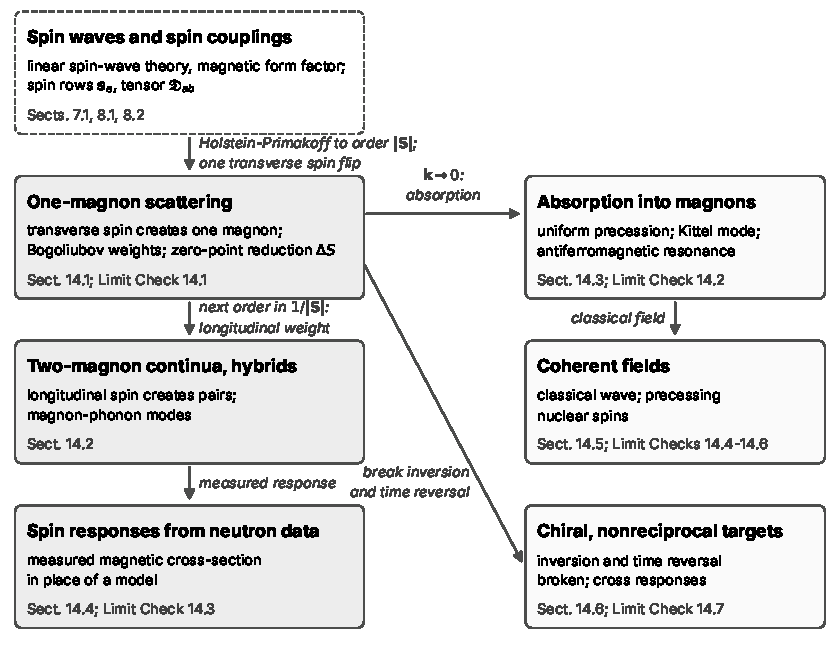
\includegraphics[width=0.85\linewidth]{figures/ch14/map14.pdf}
  \caption{Magnetic excitations, from the spin waves of \cref{sec:7.1} and the spin couplings of \cref{sec:8.1} to the targets of this chapter. A transverse spin coupling creates one magnon at leading order in $1/|\vect{S}|$, with the Bogoliubov weights of an antiferromagnet and a zero-point reduction of the ordered moment (\cref{sec:14.1}; \cref{lim:14.1a}). At the next order the longitudinal spin creates magnon pairs, and magnons mix with phonons (\cref{sec:14.2}). At vanishing momentum an absorbed boson drives the uniform precession (\cref{sec:14.3}; \cref{lim:14.3a}). The measured magnetic neutron cross-section can replace the model response (\cref{sec:14.4}; \cref{lim:14.4a}). A field whose modes are highly occupied acts as a coherent classical wave, which also drives precessing nuclear spins (\cref{sec:14.6}; \cref{lim:14.6a,lim:14.6b,lim:14.6c}). Targets that break both inversion and time reversal add chiral and nonreciprocal responses (\cref{sec:14.5}; \cref{lim:14.5a}).}
  \label{fig:14-map}
\end{figure}

\section{Magnon scattering}\label{sec:14.1}

A dark-matter particle of \SI{1}{MeV} that couples to the spin of the electron can transfer up to \SI{5.3}{keV} of momentum, twice the distance from $\Gamma$ to the ordering wavevector of NiO. It can therefore create a magnon anywhere in the zone, and \cref{sec:7.1} showed that the weight of that magnon depends strongly on where it lands: an antiferromagnet suppresses magnons near $\Gamma$ and enhances them near the ordering wavevector. Here we turn those weights into a rate, from the lightest mass that can emit a magnon above a few meV to masses where the magnetic form factor cuts it off, and we estimate the first correction in $1/|\vect{S}|$.

\subsection{One-magnon response of an antiferromagnet}

Every coupling to the electron spin in \cref{tab:8-operators}, from the contact interaction $\mathcal{O}_4 = \vect{S}_\chi\cdot\vect{S}_e$ to the velocity-dependent $\mathcal{O}_{12}$--$\mathcal{O}_{15}$, reaches the electrons through the spin row $\vect{s}_e(\vect{q})$ of \cref{eq:8.1-rows}, together with the spin current for some of them. In a magnetic insulator the spin density lives on the open shells of the ions, and \cref{eq:7.1-Fmag} replaces $\vect{s}_e(\vect{q})$ by $F^{\mathrm{mag}}(q)\sum_j\ee^{\ii\vect{q}\cdot\vect{r}_j}\vect{S}_j$, a sum over the ionic spins weighted by the magnetic form factor. We take ions whose orbital moment is quenched, as for Ni$^{2+}$; ions with an orbital moment add an orbital row (\cref{app:C.19}, \cref{sec:14.3}). At linear spin-wave order the transverse components $S^\pm$ are linear in the magnon operators and create one magnon, while $S^z$ is quadratic and creates two. The density row creates no magnon at all with the nuclei clamped, so the density--spin blocks of $S_{ab}$ vanish on one-magnon final states.

For the ferromagnet the one-magnon response is \cref{eq:7.1-Sfm}. For the antiferromagnet we need the matrix elements of $S^\pm(\vect{q})$ at any $\vect{q}$, not only near $\Gamma$ and near the ordering wavevector. \Cref{app:D.38} computes them from the operators of \cref{app:D.19}. A momentum transfer outside the zone of one sublattice is reduced by a reciprocal-lattice vector $\vect{G}$ of that sublattice, and the sites of sublattice B, displaced from those of A by $\vect{\delta}_0$, pick up the phase $\ee^{\ii\vect{G}\cdot\vect{\delta}_0} = \pm1$. That phase decides whether the two sublattices add in phase or against each other. Since $J^{\mathrm{ex}}_{\mathrm{AB}}(\vect{q})$ changes sign under a reciprocal vector of the sublattice that maps A onto B, the phase is carried automatically if the coefficients $A_{\vect{k}}$ and $B_{\vect{k}}$ of \cref{eq:7.1-Hk} are evaluated at the full momentum transfer rather than at its reduced value. The two degenerate magnons, one created by $S^-$ and one by $S^+$, precess in opposite senses and have equal weight. Inserted into \cref{eq:4.2-Sab}, their circular polarizations add to a linear one:
\begin{keyresult}[One-magnon spin response of a two-sublattice antiferromagnet]
\begin{equation}
  S_{ab}(\vect{q},\omega) = \frac{\pi|\vect{S}|}{\Omega_{\mathrm{ion}}}\,|F^{\mathrm{mag}}(q)|^2\,w^{\mathrm{M}}_{\vect{q}}\,\bigl(\delta_{ab} - \hat z_a\hat z_b\bigr)\,\delta\bigl(\omega - \omega^{\mathrm{M}}_{\vect{q}}\bigr), \qquad
  w^{\mathrm{M}}_{\vect{q}} = \frac{|\vect{S}|\,(A_{\vect{q}} - B_{\vect{q}})}{\omega^{\mathrm{M}}_{\vect{q}}} ,
  \label{eq:14.1-Safm}
\end{equation}
for $T = 0$, $\omega > 0$ and moments along $\pm\hat{\vect{z}}$, with $\Omega_{\mathrm{ion}}$ the volume per magnetic ion (for NiO the volume of the chemical primitive cell), $\omega^{\mathrm{M}}_{\vect{q}}$ of \cref{eq:7.1-afm}, and $A_{\vect{q}}$, $B_{\vect{q}}$ of \cref{eq:7.1-Hk} at the momentum transfer $\vect{q}$ itself.
\end{keyresult}
\noindent Compared to the ferromagnet of \cref{eq:7.1-Sfm}, two things change. The antisymmetric part $\ii\epsilon_{abc}\hat z_c$ is gone, because the antiferromagnet offers both senses of precession; it absorbs a transverse probe of either circular polarization. The weight is no longer one: $w^{\mathrm{M}}_{\vect{q}}$ is the factor $(u^{\mathrm{M}} \mp v^{\mathrm{M}})^2$ of \cref{eq:7.1-weights}, now written so that it holds at every $\vect{q}$ (\cref{eq:D.38-weight}). The matrix in brackets has eigenvalues $1$, $1$ and $0$, so \cref{eq:14.1-Safm} is positive semidefinite as long as $w^{\mathrm{M}}_{\vect{q}} \ge 0$, which is the stability condition $A_{\vect{q}} \ge |B_{\vect{q}}|$ of \cref{sec:7.1}.

The weight has a simple form near the two points where the magnon energy vanishes. Write $(\omega^{\mathrm{M}}_{\vect{q}})^2 = |\vect{S}|^2(A_{\vect{q}} - B_{\vect{q}})(A_{\vect{q}} + B_{\vect{q}})$. Near $\Gamma$ the sum $A + B$ tends to $2J^{\mathrm{ex}}_{\mathrm{AB}}(0)$, so
\begin{equation*}
  w^{\mathrm{M}}_{\vect{q}} \simeq \frac{\omega^{\mathrm{M}}_{\vect{q}}}{2|\vect{S}|J^{\mathrm{ex}}_{\mathrm{AB}}(0)} \quad (\vect{q} \to 0), \qquad
  w^{\mathrm{M}}_{\vect{q}} \simeq \frac{2|\vect{S}|J^{\mathrm{ex}}_{\mathrm{AB}}(0)}{\omega^{\mathrm{M}}_{\vect{q}}} \quad (\vect{q} \to \vect{Q}_{\mathrm{AF}}) ,
\end{equation*}
where near the ordering wavevector $\vect{Q}_{\mathrm{AF}}$, $(\pi/a)(1,1,1)$ in NiO, $B_{\vect{q}} \to -J^{\mathrm{ex}}_{\mathrm{AB}}(0)$ and the difference $A - B$ takes the large value instead. The scale is the exchange energy $2|\vect{S}|J^{\mathrm{ex}}_{\mathrm{AB}}(0) = 12|\vect{S}|(J_1 + J_2) = \SI{211.7}{meV}$ for NiO. A magnon of \SI{5}{meV} near $\Gamma$ carries $w^{\mathrm{M}} = 0.024$, a magnon of the same energy near $\vect{Q}_{\mathrm{AF}}$ carries 42, and a ferromagnet would give 1 to both. Physically, a long-wavelength transverse probe tries to tilt the two sublattices the same way, against the full exchange field. A probe that alternates in sign from one $(111)$ plane to the next tilts them in opposite directions, which rotates the Néel order as a whole and costs almost nothing. Evaluated within \SI{0.01}{\angstrom^{-1}} of either point, \cref{eq:14.1-Safm} agrees with these forms to \SI{0.02}{\percent}.

The exchange constants that fix $A_{\vect{q}}$, $B_{\vect{q}}$ and $\omega^{\mathrm{M}}_{\vect{q}}$ come, for NiO, from the neutron fit of \cref{eq:7.1-NiO}. For a magnet without such data they are computed in DFT~$+\,U$ by the energy-mapping, spin-spiral or Green's-function routes of \cref{app:E.9}, together with the single-ion anisotropies that open the gaps. \Cref{app:E.20-magnet} specifies these calculations for yttrium iron garnet (YIG), NiO, MnO, Cr$_2$O$_3$ and NiPS$_3$. The spread of the computed $J_2$ of NiO, 11 to \SI{27}{meV} (\cref{sec:7.1}), scales $\omega^{\mathrm{M}}$ but leaves $w^{\mathrm{M}}_{\vect{q}}$ unchanged, since the weight depends only on ratios of exchange constants. A ferrimagnet such as YIG, with 20 magnetic ions per primitive cell, needs the multi-sublattice Bogoliubov transformation in place of \cref{eq:14.1-Safm}.

\subsection{Rate formula and mass edge}

The rate follows from \cref{eq:8.2-spectrum} with $S_{ab}$ of \cref{eq:14.1-Safm} in the spin block. Since the response is proportional to $\delta_{ab} - \hat z_a\hat z_b$, the contraction picks out the part of the dark-matter tensor transverse to the moments,
\begin{equation}
  \sum_{a,b}\mathfrak{D}_{ab}S_{ab}(\vect{q},\omega) = \frac{\pi|\vect{S}|}{\Omega_{\mathrm{ion}}}\,|F^{\mathrm{mag}}(q)|^2\,w^{\mathrm{M}}_{\vect{q}}\,\bigl[\Tr\mathfrak{D} - \hat{\vect{z}}\cdot\mathfrak{D}\cdot\hat{\vect{z}}\bigr]\,\delta\bigl(\omega - \omega^{\mathrm{M}}_{\vect{q}}\bigr) ,
  \label{eq:14.1-contract}
\end{equation}
with $\mathfrak{D}_{ab}$ of \cref{eq:8.1-D} for the spin rows. For $\mathcal{O}_4$, the spin-dependent contact interaction, $\mathfrak{D}_{ab} = |c_4^{(e)}|^2\delta_{ab}/4$ for dark matter of spin $\frac12$, the bracket is $|c_4^{(e)}|^2/2$, and the rate does not depend on the direction of the moments. For $\mathcal{O}_6$, whose tensor is proportional to $q_aq_b$, the bracket is proportional to $1 - (\hat{\vect{q}}\cdot\hat{\vect{z}})^2$. Only the component of the momentum transfer perpendicular to the moments then creates a magnon, and the rate of a fixed crystal changes as the Earth turns the wind relative to the moments.

We present rates for $\mathcal{O}_4$ with a heavy mediator, $c_4^{(e)}$ independent of $q$. The reference cross-section is that of the same operator on a free electron, $\sigmae = \mu_{\chi e}^2\langle|\tilde V|^2\rangle/\pi$ as in \cref{sec:1.4}, with the average over both spins. Since $\langle|\vect{S}_\chi\cdot\vect{S}_e|^2\rangle = \sum_{a,b}\Tr(S^a_\chi S^b_\chi)\Tr(S^a_eS^b_e)/4 = 3/16$,
\begin{equation}
  \sigmae = \frac{3\mu_{\chi e}^2|c_4^{(e)}|^2}{16\pi} ,
  \label{eq:14.1-sigma}
\end{equation}
the definition of Trickle, Zhang and Zurek~\cite[Eq.~(11)]{trickle2020detecting} for this operator. The response depends on the direction of $\vect{q}$ through $w^{\mathrm{M}}_{\vect{q}}$ and $\omega^{\mathrm{M}}_{\vect{q}}$, and the full velocity kernel of \cref{app:A.8} gives the daily modulation of a fixed crystal. Averaged over the orientations of the crystal relative to the wind, the kernel is $\eta(\vmin)/2q$ per $\dd^3q/(2\pi)^3$ (\cref{eq:A.8-eta}). The rate per unit target mass above a threshold $\omega_{\mathrm{th}}$ is then
\begin{equation}
  \mathcal{R}(\omega_{\mathrm{th}}) = \frac{2\rho_\chi\sigmae|\vect{S}|}{3\,\mchi\rho_T\,\mu_{\chi e}^2\,\Omega_{\mathrm{ion}}}\int_0^{\infty}\dd q\,q\,\Bigl\langle|F^{\mathrm{mag}}(q)|^2\,w^{\mathrm{M}}_{\vect{q}}\,\eta\bigl(\vmin(q,\omega^{\mathrm{M}}_{\vect{q}})\bigr)\,\Theta\bigl(\omega^{\mathrm{M}}_{\vect{q}} - \omega_{\mathrm{th}}\bigr)\Bigr\rangle_{\hat{\vect{q}}} ,
  \label{eq:14.1-rate}
\end{equation}
with $\langle\cdots\rangle_{\hat{\vect{q}}}$ the average over the directions of $\vect{q}$ at fixed $q$ and $\vmin = \omega/q + q/2\mchi$ from \cref{eq:1.3-vmin}. The numerical factor collects $\pi|c_4^{(e)}|^2/2$ from \cref{eq:14.1-contract}, $16\pi\sigmae/3\mu_{\chi e}^2$ from \cref{eq:14.1-sigma}, and $1/4\pi^2$ from the angular integral. At $F^{\mathrm{mag}} = 1$, \cref{eq:14.1-rate} is the orientation average of the one-magnon rate of Trickle, Zhang and Zurek~\cite[Eqs.~(5)--(10)]{trickle2020detecting}, which their later work extends to all the operators of \cref{tab:8-operators}~\cite[Eqs.~(34) and~(38)]{trickle2022effective}. For one sublattice, $w^{\mathrm{M}} = 1$ and the bracket of the ferromagnet replaces that of \cref{eq:14.1-contract}; the result is their ferromagnetic rate~\cite[Eq.~(12)]{trickle2020detecting} with the spin density $|\vect{S}|/\Omega_{\mathrm{ion}}$.

The lightest mass that reaches a threshold follows from the linear dispersion near the gapless points, $\omega^{\mathrm{M}} \simeq c_{\mathrm{M}}|\vect{q} - \vect{k}_0|$ with $\vect{k}_0$ either $0$ or $\vect{Q}_{\mathrm{AF}}$ and $c_{\mathrm{M}}$ the magnon velocity. The momentum transfer from light dark matter is small, so only the region near $\Gamma$ counts. A magnon of momentum $q$ can be emitted if $c_{\mathrm{M}}q \le qv - q^2/2\mchi$, that is, for $q \le 2\mchi(v - c_{\mathrm{M}})$, and it lies above threshold for $q \ge \omega_{\mathrm{th}}/c_{\mathrm{M}}$. Both hold at the fastest speed when
\begin{equation}
  \mchi \ge \frac{\omega_{\mathrm{th}}}{2c_{\mathrm{M}}(v_{\mathrm{max}} - c_{\mathrm{M}})} ,
  \label{eq:14.1-mmin}
\end{equation}
the magnon analog of the acoustic edge of \cref{sec:11.1}. The speed $c_{\mathrm{M}} = 1.39\times10^{-4}$ of \cref{we:7-nio} is that of $J_2$ alone. With $J_1$ added, the model of \cref{fig:14-nio-rate} has speeds from $1.29\times10^{-4}$ to $1.36\times10^{-4}$ depending on direction, and the fastest puts the edge for $\omega_{\mathrm{th}} = \SI{5}{meV}$ at \SI{7.3}{keV}. Near the edge, however, the weight is $w^{\mathrm{M}} \simeq \omega_{\mathrm{th}}/2|\vect{S}|J^{\mathrm{ex}}_{\mathrm{AB}}(0) = 0.024$, and the antiferromagnet starts about forty times below a ferromagnet with the same magnon velocity.

\subsection{Zero-point spin reduction}

Linear spin-wave theory is the leading order of an expansion in $1/|\vect{S}|$, and for Ni$^{2+}$, with $|\vect{S}| = 1$, the expansion parameter $1/(2|\vect{S}|)$ is one half. The size of the first correction to \cref{eq:14.1-rate} follows from a sum rule. Each ionic spin has a fixed length, $\vect{S}_i^2 = |\vect{S}|(|\vect{S}| + 1)$, and the equal-time correlations of one site split that total into three parts. The static moment $\langle S^z_i\rangle^2$ scatters only elastically, into Bragg peaks. The transverse fluctuations $W_\perp = \langle S^x_iS^x_i + S^y_iS^y_i\rangle$ are, at linear order, all one-magnon weight. The longitudinal fluctuations $W_\parallel = \langle(S^z_i)^2\rangle - \langle S^z_i\rangle^2$ create magnon pairs. Each weight is the integral of the corresponding block of $S_{ab}$ over $\omega$ and over the zone. Together they fix how the spectral weight that a spin coupling can reach is divided between the one-magnon line, the two-magnon continuum and the elastic peaks, which deposit no energy.

In the Néel state the transverse fluctuations would be $|\vect{S}|$ and the longitudinal ones zero. The true ground state is not the Néel state. The pair term of \cref{eq:7.1-Hk} mixes in states with a deviation on each sublattice, and each mode leaves the zero-point deviation $(v^{\mathrm{M}}_{\vect{k}})^2$ on every site (\cref{sec:7.1}). \Cref{app:D.38} evaluates the three weights in this ground state, the longitudinal one by Wick's theorem:
\begin{keyresult}[Spin weights at linear spin-wave order]
\begin{equation}
  \begin{gathered}
  \Delta S = \frac{1}{N_{\mathrm{s}}}\sum_{\vect{k}}\bigl(v^{\mathrm{M}}_{\vect{k}}\bigr)^2, \qquad
  W_\perp = |\vect{S}|\,(1 + 2\Delta S), \qquad
  W_\parallel = \Delta S\,(1 + \Delta S), \\
  \frac{W_\parallel}{W_\perp} = \frac{\Delta S\,(1 + \Delta S)}{|\vect{S}|\,(1 + 2\Delta S)} ,
  \end{gathered}
  \label{eq:14.1-ratio}
\end{equation}
with the sum over the zone of one sublattice and the ordered moment $\langle S^z_i\rangle = |\vect{S}| - \Delta S$.
\end{keyresult}
\noindent The zero-point spin reduction $\Delta S$ depends on the lattice and on ratios of exchange constants, not on $|\vect{S}|$, so the ratio falls as $1/|\vect{S}|$ with a coefficient fixed by the lattice. For a ferromagnet $v^{\mathrm{M}}_{\vect{k}} = 0$, and both $\Delta S$ and $W_\parallel$ vanish: the fully polarized state is exact, and a longitudinal probe finds nothing to excite. For an antiferromagnet the zone average of the weight $w^{\mathrm{M}}_{\vect{q}}$ of \cref{eq:14.1-Safm} is $1 + 2\Delta S$, which is the same statement as $W_\perp$, and gives a check of any numerical evaluation of the one-magnon response.

The three weights violate the sum rule. Added up, $W_\perp + W_\parallel + \langle S^z_i\rangle^2$ exceeds $|\vect{S}|(|\vect{S}| + 1)$ by $\Delta S(1 + 2\Delta S)$, because linear spin-wave theory replaces the square roots of the Holstein--Primakoff transformation \cref{eq:7.1-HP} by their value at zero deviation. Holding the ordered moment and $W_\parallel$ at the values of \cref{eq:14.1-ratio}, the sum rule requires the transverse weight $(|\vect{S}| - \Delta S)(1 + 2\Delta S)$, and \cref{app:D.38} shows that the full square roots, evaluated in the same ground state, give exactly this value. At this order, with $\langle S^z_i\rangle$ and $W_\parallel$ held at their linear spin-wave values, the one-magnon weight of linear spin-wave theory is too large by the fraction $\Delta S/|\vect{S}|$. This is an estimate of the leading correction, not a bound. The corrected transverse operator also creates three magnons, which lowers the one-magnon part further; however, the change of the ground state at the same order, which moves $\langle S^z_i\rangle$ and $W_\parallel$ as well, is not part of the estimate. The one-magnon and two-magnon weights together, $(|\vect{S}| - \Delta S)(1 + 2\Delta S) + \Delta S(1 + \Delta S) = |\vect{S}|(1 + 2\Delta S) - \Delta S^2$, agree with the linear spin-wave one-magnon weight up to $\Delta S^2$. The first correction does not remove weight; it moves the fraction $\Delta S/|\vect{S}|$ of it from the one-magnon line into the two-magnon continuum, which lies at other energies for the same momentum transfer (\cref{sec:14.2}).

\begin{workedexample}{The zero-point spin reduction of NiO}\label{we:14-nio}
For the type-II order of NiO with the exchange constants \cref{eq:7.1-NiO}, $(v^{\mathrm{M}}_{\vect{k}})^2 = \frac12[A_{\vect{k}}(A_{\vect{k}}^2 - B_{\vect{k}}^2)^{-1/2} - 1]$ with $A_{\vect{k}}$ and $B_{\vect{k}}$ of \cref{eq:7.1-Hk}. We average it over a $100^3$ grid of the cube of side $4\pi/a$, the period of the reciprocal lattice of the nickel ions along each cube axis, which holds every wavevector of the zone twice, and find
\begin{equation*}
  \Delta S = 0.0784 .
\end{equation*}
The grid avoids the gapless points at $\Gamma$ and $\vect{Q}_{\mathrm{AF}}$, where $(v^{\mathrm{M}})^2$ diverges as the inverse distance; this singularity is integrable. The sum changes by $1.1\times10^{-4}$ from $60^3$ to $80^3$ points and by $5\times10^{-5}$ from $80^3$ to $100^3$, as the inverse square of the grid size, and extrapolates to 0.0785. With $J_1 = 0$ it is $0.0783$. The reason is that the next-nearest neighbors at $\pm a\hat{\vect{x}}$, $\pm a\hat{\vect{y}}$, $\pm a\hat{\vect{z}}$ link the fcc lattice into four interpenetrating simple-cubic lattices of side $a$, each a Néel antiferromagnet. Their zero-point reduction is Anderson's 0.078 for the simple-cubic antiferromagnet~\cite{anderson1952approximate}, and the weak $J_1$ barely changes it.

With $|\vect{S}| = 1$, the ordered moment is $|\vect{S}| - \Delta S = 0.9216$ of its classical value, and \cref{eq:14.1-ratio} gives
\begin{equation*}
  W_\perp = 1.157, \qquad W_\parallel = 0.0846, \qquad \frac{W_\parallel}{W_\perp} = \frac{0.0784 \times 1.0784}{1 \times 1.1569} = 0.0731 .
\end{equation*}
The sum rule requires $W_\perp = 0.9216 \times 1.1569 = 1.066$: at this order the one-magnon weight of linear spin-wave theory, and with it the rate \cref{eq:14.1-rate}, is high by about $\Delta S/|\vect{S}| = \SI{7.8}{\percent}$. The two-magnon continuum holds \SI{7.3}{\percent} of the linear spin-wave one-magnon weight, and the total, one-magnon plus two-magnon, is $0.995$ of it. The ratio $\Delta S/|\vect{S}| = 0.078$ is six times smaller than the expansion parameter $1/(2|\vect{S}|) = 0.5$. In three dimensions the zero-point motion of the spin waves is small, and the expansion in $1/|\vect{S}|$ converges faster than its parameter suggests.
\end{workedexample}

\Cref{lim:14.1a} sets the literature rate against these weights as $|\vect{S}|$ varies at the fixed lattice and exchange ratios of NiO, where $\Delta S = 0.078$ throughout.
\begin{limitbox}[One-magnon rate at linear spin-wave order][lim:14.1a]
$\varGamma(\vect{v}) = \int\frac{\dd^3q}{(2\pi)^3}\sum_{a,b}\mathfrak{D}_{ab}S_{ab}(\vect{q},\omega_{\vect{q}})$ with the one-magnon response \cref{eq:14.1-Safm} at $F^{\mathrm{mag}} = 1$, spectral weight $W_\perp = |\vect{S}|(1 + 2\Delta S)$ per ion~\cites[Eqs.~(5)--(12)]{trickle2020detecting}[Eq.~(38)]{trickle2022effective}.
\par\smallskip
{\centering
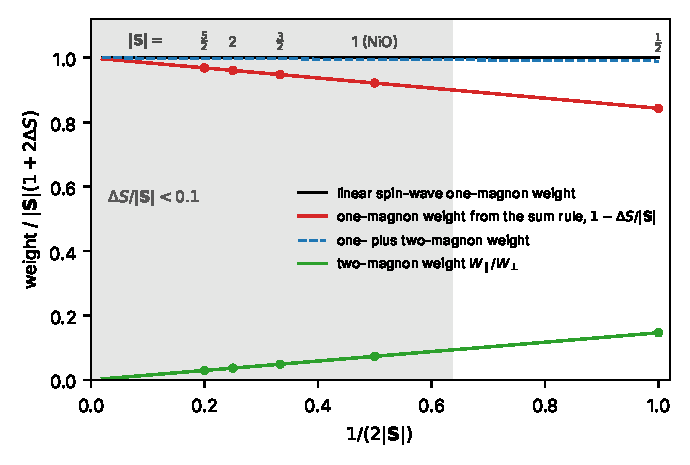
\includegraphics[width=0.92\linewidth]{figures/ch14/limit14_1a.pdf}
\captionof{figure}{Spectral weights of the spin of one magnetic ion against the expansion parameter $1/(2|\vect{S}|)$, in units of the one-magnon weight of linear spin-wave theory, $|\vect{S}|(1 + 2\Delta S)$, which the literature rate contains (black line). Red: the one-magnon weight that the sum rule $\vect{S}^2 = |\vect{S}|(|\vect{S}| + 1)$ requires, $1 - \Delta S/|\vect{S}|$. Green: the two-magnon weight $W_\parallel/W_\perp$ of \cref{eq:14.1-ratio}. Dashed: one- plus two-magnon weight, $1 - \Delta S^2/[|\vect{S}|(1 + 2\Delta S)]$. Lattice and exchange ratios of NiO (type-II order, $J_1/J_2 = -0.072$), zero-point reduction $\Delta S = 0.078$ from a $100^3$ grid; points at $|\vect{S}| = \frac12$, 1 (NiO), $\frac32$, 2 and $\frac52$. Gray: $\Delta S/|\vect{S}| < 0.1$, which holds for $|\vect{S}| \ge 0.78$.}\label{fig:14-limit-magnon}
\par}
\smallskip
For $|\vect{S}| = \frac12$ the one-magnon line is overcounted by about \SI{16}{\percent} at this order and the two-magnon weight reaches \SI{15}{\percent}, and the magnon interactions of the next order, which shift and broaden the magnons, are no longer small.
\end{limitbox}

For Mn$^{2+}$ and Fe$^{3+}$, with $|\vect{S}| = \frac52$, the same lattice gives a defect of \SI{3.1}{\percent} and a two-magnon weight of \SI{2.9}{\percent}. The rates of this section use the exchange fitted to the measured magnons, so the shift of the magnon energies by the quartic terms of the Holstein--Primakoff expansion is already absorbed into $J_1$ and $J_2$ (\cref{we:7-nio}). The division of weight in \cref{fig:14-limit-magnon} is not.

\subsection{The one-magnon rate of NiO}

The inputs for NiO are those of \cref{sec:7.1}: the exchange constants \cref{eq:7.1-NiO}, $|\vect{S}| = 1$, and $a = \SI{4.17}{\angstrom}$, so that the volume per nickel ion is $\Omega_{\mathrm{ion}} = a^3/4 = \SI{18.13}{\angstrom^3}$ and the density, from four formula units per cubic cell, is $\rho_T = \SI{6.84}{g.cm^{-3}}$. The form factor of Ni$^{2+}$, whose orbital moment is quenched, is the spin-only $F^{\mathrm{mag}} = \langle j_0(q)\rangle$ of \cref{eq:C.19-spinonly}. We take $\langle j_0\rangle$ from the tabulated fit $A\ee^{-\alpha s^2} + B\ee^{-\beta s^2} + C\ee^{-\gamma s^2} + D$ with $s = q/4\pi$, in \si{\angstrom^{-1}}, and the coefficients $(A, \alpha, B, \beta, C, \gamma, D) = (0.0163, 35.88, 0.3916, 13.22, 0.6052, 4.339, -0.0133)$~\cite[Sect.~4.4.5, Table~4.4.5.2]{anderson2006neutron}. It gives $|F^{\mathrm{mag}}|^2 = 0.84$ at $|\vect{Q}_{\mathrm{AF}}| = \SI{2.6}{keV}$ and 0.49 at \SI{5.3}{keV}, the largest momentum transfer of a \SI{1}{MeV} particle.

Two limits fix the shape of the rate before any integral is done. At the light end, \cref{eq:14.1-mmin} sets the edge, and above it the weight near $\Gamma$ grows in proportion to the magnon energy. At the heavy end, the momentum transfers sweep many zones and the magnon energies, at most \SI{118}{meV}, are negligible against $qv$. Then $\vmin \simeq q/2\mchi$, the direction average of $w^{\mathrm{M}}_{\vect{q}}$ over a shell that crosses many zones tends to its zone average $1 + 2\Delta S$, and $\int\dd q\,q\,\eta(q/2\mchi) = 4\mchi^2\int\dd u\,u\,\eta(u) = 2\mchi^2\langle v\rangle$, with $\langle v\rangle$ the mean speed of the dark matter in the laboratory. \Cref{eq:14.1-rate} at $F^{\mathrm{mag}} = 1$ becomes
\begin{equation}
  \mathcal{R} \simeq \frac{\rho_\chi}{\mchi}\,\frac{\langle v\rangle}{\rho_T\Omega_{\mathrm{ion}}}\,\sigmae\Bigl(\frac{\mchi}{\mu_{\chi e}}\Bigr)^2\,\frac{|\vect{S}|(1 + 2\Delta S)}{3/4} .
  \label{eq:14.1-inc}
\end{equation}
This is the flux of dark matter times the number of ions per unit mass times a cross-section per ion. At large $q$ the magnet looks like a gas of free spins, each with the transverse weight $W_\perp$ in place of the electron's $\frac34$, and with the reduced mass $\mu_{\chi e}$ replaced by $\mchi$ for a heavy target. With $\langle v\rangle = \SI{354}{km/s}$ for the halo of \cref{sec:1.2}, the integral \cref{eq:14.1-rate} at $F^{\mathrm{mag}} = 1$ is 0.96 of \cref{eq:14.1-inc} at \SI{3}{MeV} and 0.989 at \SI{10}{MeV}.

\begin{figure}[tbp]
  \centering
  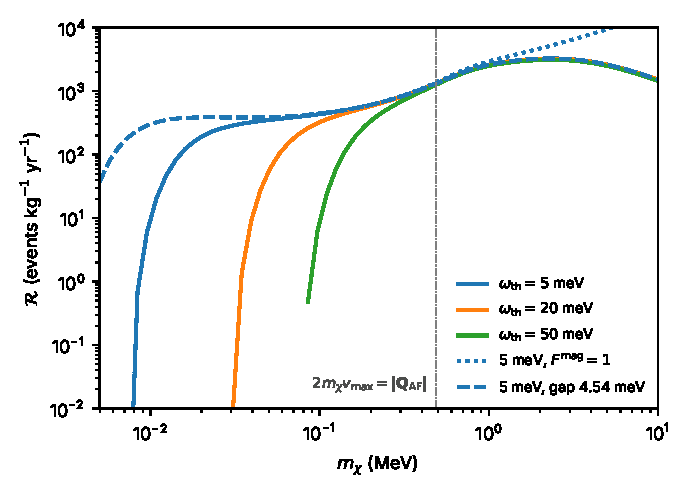
\includegraphics[width=0.75\linewidth]{figures/ch14/fig14_1.pdf}
  \caption{One-magnon rate of NiO per kilogram-year for dark matter with the spin-dependent contact interaction $\mathcal{O}_4 = \vect{S}_\chi\cdot\vect{S}_e$ (heavy mediator) at the reference cross-section $\sigmae = \SI{e-40}{cm^2}$ of \cref{eq:14.1-sigma}, against the dark-matter mass, from \cref{eq:14.1-rate}: $T = 0$, rate averaged over the orientations of the crystal relative to the dark-matter wind, standard halo of \cref{sec:1.2}. Solid: energy thresholds of 5, 20 and \SI{50}{meV}. Model: Heisenberg exchange $J_1 = -\SI{1.37}{meV}$, $J_2 = \SI{19.01}{meV}$ from neutron scattering, $|\vect{S}| = 1$, $a = \SI{4.17}{\angstrom}$, undistorted fcc lattice without anisotropy (gapless), linear spin-wave theory, magnetic form factor of Ni$^{2+}$. Dotted: \SI{5}{meV} threshold without the form factor, $F^{\mathrm{mag}} = 1$. Dashed: \SI{5}{meV} threshold with an easy-axis single-ion anisotropy added to $A_{\vect{k}}$ and chosen to put the zone-center gap at \SI{4.54}{meV}, the zone-center magnon of NiO seen in far-infrared absorption. Vertical line: the mass at which the largest momentum transfer, $2\mchi v_{\mathrm{max}}$, reaches the ordering wavevector, \SI{0.49}{MeV}.}
  \label{fig:14-nio-rate}
\end{figure}

\Cref{fig:14-nio-rate} shows the full integral. At a threshold of \SI{5}{meV} the rate rises from the edge, at \SI{7.4}{keV} on the mass grid of the figure, to 10 events per kilogram-year at \SI{10}{keV}, 280 at \SI{30}{keV} and 430 at \SI{100}{keV}, for $\sigmae = \SI{e-40}{cm^2}$. At \SI{100}{keV} all of it comes from momentum transfers within half the distance to $\vect{Q}_{\mathrm{AF}}$, where the weight is suppressed. Once the momentum transfer reaches the ordering wavevector the enhanced magnons there take over, and at \SI{1}{MeV}, where the rate is $2.6\times10^3$, only \SI{19}{\percent} of it comes from the region near $\Gamma$. The rate peaks at $3.2\times10^3$ near \SI{3}{MeV} and then falls, because the form factor removes the momentum transfers beyond the inverse radius of the $3d$ shell. It costs a factor 0.89 at \SI{1}{MeV}, and a factor 11.4 against $F^{\mathrm{mag}} = 1$ at \SI{10}{MeV}, where the rate is $1.5\times10^3$. The threshold matters only for the lightest masses. Above \SI{0.3}{MeV} the rates at 5, 20 and \SI{50}{meV} differ by less than \SI{20}{\percent}, since most of the rate then comes from magnons above \SI{50}{meV}. Below, the higher thresholds push the edge up to \SI{30}{keV} and \SI{85}{keV}. The second is later than \cref{eq:14.1-mmin} gives for \SI{50}{meV}, because the dispersion bends over below its maximum.

Near its gap the rate depends on what the Heisenberg model leaves out. Magnetic anisotropy, which \cref{sec:7.1} neglected, lifts the Goldstone modes at $\Gamma$ and $\vect{Q}_{\mathrm{AF}}$ to energies below \SI{5}{meV}. The undistorted $J_1$--$J_2$ model also has a third, accidental zero at $\mathrm{X} = (2\pi/a)(1,0,0)$, where $A_{\vect{k}} = B_{\vect{k}} = 6J_2 - 2J_1$; the weight vanishes there, and the rhombohedral distortion of the real crystal lifts it. Far-infrared absorption places a zone-center magnon of NiO at \SI{4.54}{meV}, the value used by Hutchings and Samuelsen~\cite{hutchings1972measurement} and quoted by dos Santos and collaborators~\cite[Sect.~III]{dossantos2026comparative}. We add an easy-axis term $K$ to $A_{\vect{k}}$, which keeps the form of \cref{eq:7.1-Hk}, and choose $K = \SI{0.0973}{meV}$ so that $|\vect{S}|[(A_0 + K)^2 - A_0^2]^{1/2} = \SI{4.54}{meV}$. With a \SI{5}{meV} threshold the rate then grows by a factor of 29 at \SI{10}{keV} and 1.35 at \SI{30}{keV}, and changes by less than \SI{3}{\percent} above \SI{100}{keV}. The gap puts magnons just above threshold at vanishing momentum, where the kinematics is easiest, and their weight $K^{1/2}/(2A_0)^{1/2}$ is set by the anisotropy. For dark matter lighter than about \SI{50}{keV}, the rate of NiO near its gap is set by its anisotropy. The real anisotropy is biaxial: it keeps the moments in the $(111)$ planes (\cref{fig:7-nio}) and gaps the two branches differently, so that only one of them reaches \SI{4.54}{meV} while the in-plane branch lies near \SI{0.6}{meV}. The one-constant model gaps both at \SI{4.54}{meV}, and the factor 29 is an upper value. The anisotropy enters through the uniform modes of \cref{sec:14.3} and the anisotropy constants of \cref{app:E.20-magnet}. Temperature adds thermal magnons with occupation $\ee^{-\omega^{\mathrm{M}}/T}$; at the gap of \SI{4.54}{meV} the exponent is $-5\times10^3$ at \SI{10}{mK} and $-53$ at \SI{1}{K}, and the zero-temperature response holds at any cryogenic operating point.

\section{Two-magnon continua and magnon--phonon modes}\label{sec:14.2}

In NiO, linear spin-wave theory assigns to the component of each nickel spin along the ordered moment a fluctuation weight equal to \SI{7}{\percent} of the one-magnon weight (\cref{we:14-nio}), carried entirely by magnon pairs, which that component creates (\cref{sec:7.1}). Each pair shares the momentum transfer between its two members, so at a small momentum transfer the pair can take up any energy from the one-magnon energy to twice the top of the magnon band, \SI{236}{meV}. The pairs thus decouple the energy deposited from the momentum transfer, which matters for the lightest dark matter. In the effective theory of gapless antiferromagnetic magnons, the two-magnon channel extends the projected reach of NiO, MnO and Cr$_2$O$_3$ down to masses of about \SI{1}{keV}~\cite{esposito2023optimal}. The lattice adds a second correction. Through spin--orbit coupling a strain changes the magnetic anisotropy energy, and a magnon and a phonon of the same wavevector and energy mix into hybrid modes. Together with the one-magnon weight defect of \cref{sec:14.1}, the pairs, their final-state interaction and the hybrids are the corrections in $1/|\vect{S}|$ and in the magnetoelastic coupling to the one-magnon rate, and for NiO we size each.

\subsection{Two-magnon amplitude and response}\label{sec:14.2-amp}

Take the two-sublattice antiferromagnet of \cref{sec:7.1}, with the moments along $\pm\hat{\vect{z}}$, and the longitudinal ionic spin at wavevector $\vect{q}$, $S^z(\vect{q}) = \sum_j\ee^{\ii\vect{q}\cdot\vect{r}_j}S^z_j$. On sublattice A, $S^z_i = |\vect{S}| - d^\dagger_{\mathrm{A}i}d_{\mathrm{A}i}$, and on B, $S^z_j = -|\vect{S}| + d^\dagger_{\mathrm{B}j}d_{\mathrm{B}j}$, exactly, by \cref{eq:7.1-HP}. The constants give the magnetic Bragg peaks, at $\omega = 0$, and deposit no energy. The rest is bilinear in the bosons. With the Fourier convention of \cref{sec:7.1} on each sublattice, the lattice sums give
\begin{equation*}
  S^z(\vect{q}) = -\sum_{\vect{k}}d^\dagger_{\mathrm{A}\vect{k}}\,d_{\mathrm{A},\vect{k}-\vect{q}} + \sum_{\vect{k}}d^\dagger_{\mathrm{B}\vect{k}}\,d_{\mathrm{B},\vect{k}+\vect{q}} + (\text{Bragg}) ,
\end{equation*}
with $\vect{k}$ over the $N_{\mathrm{s}}$ wavevectors of the zone of one sublattice. Now insert the inverse Bogoliubov transformation \cref{eq:D.19-inverse}, $d_{\mathrm{A}\vect{k}} = u^{\mathrm{M}}_{\vect{k}}a_{\vect{k}1} - v^{\mathrm{M}}_{\vect{k}}a^\dagger_{\vect{k}2}$ and $d_{\mathrm{B}\vect{k}} = u^{\mathrm{M}}_{\vect{k}}a_{\vect{k}2} - v^{\mathrm{M}}_{\vect{k}}a^\dagger_{\vect{k}1}$. At $T = 0$ only the terms with two creation operators survive acting on the magnon vacuum $|0\rangle$. The A term contributes $u^{\mathrm{M}}_{\vect{k}}v^{\mathrm{M}}_{\vect{k}-\vect{q}}\,a^\dagger_{\vect{k}1}a^\dagger_{\vect{k}-\vect{q},2}$, and the B term, after the relabeling $\vect{k} + \vect{q} \to \vect{k}$, contributes $-v^{\mathrm{M}}_{\vect{k}}u^{\mathrm{M}}_{\vect{k}-\vect{q}}$ times the same pair. Hence
\begin{equation}
  S^z(\vect{q})|0\rangle = \sum_{\vect{k}}\mathcal{A}^{\mathrm{2m}}_{\vect{k}}(\vect{q})\,a^\dagger_{\vect{k}1}a^\dagger_{\vect{k}-\vect{q},2}|0\rangle , \qquad
  \mathcal{A}^{\mathrm{2m}}_{\vect{k}}(\vect{q}) = u^{\mathrm{M}}_{\vect{k}}v^{\mathrm{M}}_{\vect{k}-\vect{q}} - v^{\mathrm{M}}_{\vect{k}}u^{\mathrm{M}}_{\vect{k}-\vect{q}} ,
  \label{eq:14.2-amp}
\end{equation}
apart from the Bragg term. The first magnon carries the crystal momentum $\vect{k}$ and lowers the total $S^z$ by one; the second carries $\vect{q} - \vect{k}$, since $a_{\vect{k}2}$ destroys $-\vect{k}$ in the convention of \cref{sec:7.1}, and raises $S^z$ by one. The pair has the momentum $\vect{q}$ and no net spin, as a longitudinal operator requires. The wavevector $\vect{k} - \vect{q}$ may leave the zone of one sublattice. We then compute $u^{\mathrm{M}}$ and $v^{\mathrm{M}}$ at that wavevector from $A_{\vect{k}}$ and $B_{\vect{k}} = J^{\mathrm{ex}}_{\mathrm{AB}}(\vect{k})$ with its sign. Since $J^{\mathrm{ex}}_{\mathrm{AB}}$ changes by at most a sign under a reciprocal vector of the sublattice, $v^{\mathrm{M}}$ does too, and $|\mathcal{A}^{\mathrm{2m}}_{\vect{k}}|^2$ does not depend on which representative is used.

A ferromagnet has $v^{\mathrm{M}} \equiv 0$ and no amplitude, and at $T = 0$ no inelastic longitudinal response at all, beyond linear order as well (\cref{sec:14.1}). In an antiferromagnet the amplitude vanishes at $\vect{q} = 0$, where $u_{\vect{k}}v_{\vect{k}} - v_{\vect{k}}u_{\vect{k}} = 0$, and at every reciprocal vector of the lattice of magnetic ions, where $S^z(\vect{q})$ is the total $S^z$, which commutes with $H_{\mathrm{H}}$ and creates nothing. For small $\vect{q}$, with $u^{\mathrm{M}} = \cosh\theta_{\vect{k}}$ and $v^{\mathrm{M}} = \sinh\theta_{\vect{k}}$, the amplitude is $\mathcal{A}^{\mathrm{2m}}_{\vect{k}} = \sinh(\theta_{\vect{k}-\vect{q}} - \theta_{\vect{k}}) \simeq -\vect{q}\cdot\nabla_{\vect{k}}\theta_{\vect{k}}$, and the weight grows as $q^2$. Near the ordering wavevector $v^{\mathrm{M}}_{\vect{k}-\vect{q}}$ has the opposite sign to $v^{\mathrm{M}}_{\vect{k}}$, the two terms add, and the amplitude approaches $2u^{\mathrm{M}}_{\vect{k}}v^{\mathrm{M}}_{\vect{k}} = \sinh2\theta_{\vect{k}}$, its largest value. Physically, $S^z(\vect{q})$ near the ordering wavevector measures the fluctuation of the staggered moment, which the zero-point motion of the spin waves makes large.

The response follows as in \cref{sec:7.1}. The electron spin density along the moments is $s_{e,z}(\vect{q}) = F^{\mathrm{mag}}(q)S^z(\vect{q})$ by \cref{eq:7.1-Fmag}. The pair states of \cref{eq:14.2-amp} are orthonormal, and each appears once in the sum over $\vect{k}$. With $N = 2N_{\mathrm{s}}$ magnetic ions, $\Omega_{\mathrm{ion}}$ the volume per ion and $\Vol = N\Omega_{\mathrm{ion}}$, \cref{eq:4.2-Sab} gives:
\begin{keyresult}[Two-magnon spin response of a collinear antiferromagnet]
\begin{equation}
  S^{(2\mathrm{m})}_{zz}(\vect{q},\omega) = \frac{2\pi}{\Omega_{\mathrm{ion}}}\,|F^{\mathrm{mag}}(q)|^2\,\frac{1}{2N_{\mathrm{s}}}\sum_{\vect{k}}\bigl|\mathcal{A}^{\mathrm{2m}}_{\vect{k}}(\vect{q})\bigr|^2\,\delta\bigl(\omega - \omega^{\mathrm{M}}_{\vect{k}} - \omega^{\mathrm{M}}_{\vect{k}-\vect{q}}\bigr) ,
  \label{eq:14.2-S2m}
\end{equation}
for $T = 0$ and $\omega > 0$, with $z$ along the moments and $\mathcal{A}^{\mathrm{2m}}$ of \cref{eq:14.2-amp}. Its weight and that of the one-magnon line at the same $\vect{q}$ are in the ratio $w_\parallel(\vect{q})/w_\perp(\vect{q})$ of the weights per ion
\begin{equation}
  w_\parallel(\vect{q}) = \frac{1}{2N_{\mathrm{s}}}\sum_{\vect{k}}\bigl|\mathcal{A}^{\mathrm{2m}}_{\vect{k}}(\vect{q})\bigr|^2 , \qquad
  w_\perp(\vect{q}) = |\vect{S}|\,w^{\mathrm{M}}_{\vect{q}} ,
  \label{eq:14.2-wpar}
\end{equation}
with $w^{\mathrm{M}}_{\vect{q}}$ the one-magnon weight of \cref{eq:14.1-Safm}.
\end{keyresult}
\noindent Here $w_\perp$ is the $\omega$-integral of $S_{xx} + S_{yy}$ in units of $(2\pi/\Omega_{\mathrm{ion}})|F^{\mathrm{mag}}|^2$. The one-magnon weight is of order $|\vect{S}|$ and the two-magnon weight of order $|\vect{S}|^0$, since the Bogoliubov coefficients do not depend on $|\vect{S}|$: the pairs are a correction of relative order $1/|\vect{S}|$. \Cref{eq:14.2-S2m} is the longitudinal structure factor that Huberman and collaborators compared with the two-magnon continuum of the square-lattice antiferromagnet Rb$_2$MnF$_4$ measured by neutron scattering~\cite[Eq.~(5)]{huberman2005two}. A dark-matter model enters through $\mathfrak{D}_{zz}S^{(2\mathrm{m})}_{zz}$ in \cref{eq:8.2-spectrum}, in the frame of the moments. For a coupling isotropic in the electron spin, $\mathfrak{D}_{ab} \propto \delta_{ab}$, the two-magnon and one-magnon parts of $\sum_a\mathfrak{D}_{aa}S_{aa}$ at fixed $\vect{q}$ are in the ratio $w_\parallel/w_\perp$, whatever the direction of the moments in each domain.

Averaged over $\vect{q}$, $v^{\mathrm{M}}_{\vect{k}-\vect{q}}$ takes both signs equally often, the cross term of $|\mathcal{A}^{\mathrm{2m}}|^2$ drops out, and with $\langle(u^{\mathrm{M}})^2\rangle = 1 + \Delta S$ and $\langle(v^{\mathrm{M}})^2\rangle = \Delta S$, where $\Delta S$ is the zero-point spin reduction of \cref{sec:14.1}, the average of $w_\parallel$ is $\frac12\cdot2(1 + \Delta S)\Delta S = W_\parallel$, while the average of $w_\perp$ is $|\vect{S}|(1 + 2\Delta S) = W_\perp$. \Cref{eq:14.2-wpar} thus resolves the ratio $W_\parallel/W_\perp$ of \cref{sec:14.1} in momentum transfer, which is what a rate needs, since light dark matter samples only small $q$.

\Cref{fig:14-weights} shows the two weights of NiO in linear spin-wave theory with the exchange constants of \cref{eq:7.1-NiO}. At small $q$ along $[111]$ the one-magnon weight rises as $w_\perp \simeq 0.29\,qa$, and the two-magnon weight as $w_\parallel \simeq 0.015\,(qa)^2$, so the ratio vanishes linearly. At $\vect{q} = (\frac14,\frac14,\frac14)2\pi/a$, a momentum transfer of \SI{1.29}{keV}, $w_\perp = 1.00$ and $w_\parallel = 0.081$; along $[111]$ the ratio $w_\parallel/w_\perp$ peaks at 0.082 near \SI{1.4}{keV} and stays below 0.05 under \SI{0.5}{keV}. Toward the ordering wavevector $w_\perp$ diverges while $w_\parallel$ stays finite, near 0.25, and the ratio falls again, averaging over the zone to the $W_\parallel/W_\perp$ of \cref{we:14-nio}.

\begin{figure}[tbp]
  \centering
  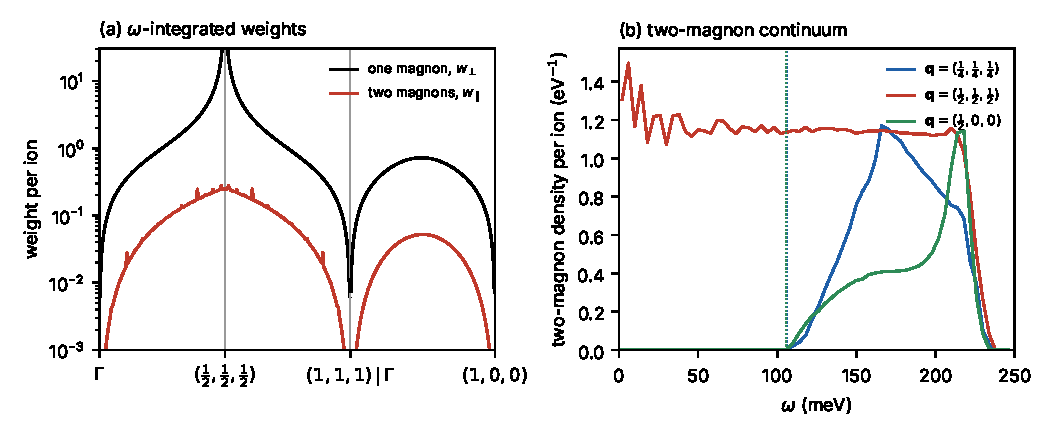
\includegraphics[width=\linewidth]{figures/ch14/fig14_2.pdf}
  \caption{One- and two-magnon weights of NiO in linear spin-wave theory: Heisenberg model with $J_1 = \SI{-1.37}{meV}$ and $J_2 = \SI{19.01}{meV}$ (antiferromagnetic $J^{\mathrm{ex}} > 0$, pairs counted once), $|\vect{S}| = 1$, type-II order on the undistorted fcc lattice, no anisotropy, $T = 0$, magnetic form factor set to one. (a) Weights per ion, integrated over energy, of the transverse one-magnon response, $w_\perp$ (both branches), and of the longitudinal two-magnon response, $w_\parallel$. The path runs along $[111]$ from $\Gamma$ through the ordering wavevector $(\frac12,\frac12,\frac12)$ to $(1,1,1)$, which is equivalent to $\Gamma$, and from $\Gamma$ to $(1,0,0)$; wavevectors in units of $2\pi/a$, $a = \SI{4.17}{\angstrom}$. Both vanish at $\Gamma$ and $(1,1,1)$, where the total longitudinal spin is conserved; $w_\perp$ diverges at the ordering wavevector and vanishes at $(1,0,0)$, a soft point of the undistorted model, where $w_\parallel$ is small and would vanish for $J_1 = 0$. (b) Two-magnon density per ion, $(\Omega_{\mathrm{ion}}/2\pi)S^{(2\mathrm{m})}_{zz}/|F^{\mathrm{mag}}|^2$, against energy at three wavevectors (4-meV bins, $3\times10^6$ sampled wavevectors). The dotted lines mark the one-magnon energy at the same wavevector, zero at the ordering wavevector.}
  \label{fig:14-weights}
\end{figure}

\subsection{Kinematic boundaries of the continuum}\label{sec:14.2-edges}

At fixed $\vect{q}$, \cref{eq:14.2-S2m} has weight only between the lower edge $\omega_-(\vect{q}) = \min_{\vect{k}}(\omega^{\mathrm{M}}_{\vect{k}} + \omega^{\mathrm{M}}_{\vect{k}-\vect{q}})$ and the upper edge $\omega_+(\vect{q}) = \max_{\vect{k}}(\omega^{\mathrm{M}}_{\vect{k}} + \omega^{\mathrm{M}}_{\vect{k}-\vect{q}}) \le 2\max_{\vect{k}}\omega^{\mathrm{M}}_{\vect{k}}$. Putting one magnon at a zero of the dispersion, $\vect{k} = 0$, shows that $\omega_- \le \omega^{\mathrm{M}}_{\vect{q}}$; for a dispersion that rises linearly and then bends over, as in NiO, $\omega^{\mathrm{M}}_{\vect{k}} + \omega^{\mathrm{M}}_{\vect{k}-\vect{q}} \ge \omega^{\mathrm{M}}_{\vect{q}}$, and the lower edge is the one-magnon branch itself. The weight at the lower edge is small, because $|\mathcal{A}^{\mathrm{2m}}|^2$ diverges only as $1/k$ near $\vect{k} = 0$ while the phase space closes as $k^2$. In NiO the continuum at $(\frac14,\frac14,\frac14)2\pi/a$ runs from the one-magnon energy, \SI{105.8}{meV}, to \SI{236}{meV}, and at the ordering wavevector it runs from zero, where both magnons sit at zeros of the dispersion, to \SI{236}{meV} (\cref{fig:14-weights}b). The anisotropy that \cref{eq:7.1-heis} leaves out gaps the magnons by less than \SI{5}{meV} in NiO; a gap $\omega_{\mathrm{gap}}$ in both branches moves the lower edge to at least $2\omega_{\mathrm{gap}}$ and leaves the rest of the continuum in place. At $T > 0$ the operator $S^z$ also scatters a thermal magnon into another, with weight proportional to the occupation, which vanishes for temperatures far below the gap.

The continuum changes what dark matter can deposit. Energy conservation, \cref{eq:1.3-omegaq}, allows $\omega \le qv - q^2/2\mchi$, and the one-magnon channel opens at \cref{eq:14.1-mmin}. A pair, however, can take any energy in its continuum, which at small $q$ reaches far above $c_{\mathrm{M}}q$, so the only limit is \cref{eq:1.3-omegamax}, $\omega \le \frac12\mchi v^2$, reached at $q = \mchi v$. For a threshold $E_{\mathrm{th}}$ the two-magnon channel opens at the threshold mass \cref{eq:1.3-mmin}, $2E_{\mathrm{th}}/v_{\mathrm{max}}^2$. The one-magnon channel opens at $E_{\mathrm{th}}/[2c_{\mathrm{M}}(v_{\mathrm{max}} - c_{\mathrm{M}})]$, larger by the factor
\begin{equation}
  \frac{v_{\mathrm{max}}^2}{4c_{\mathrm{M}}(v_{\mathrm{max}} - c_{\mathrm{M}})} \simeq \frac{v_{\mathrm{max}}}{4c_{\mathrm{M}}} \qquad (c_{\mathrm{M}} \ll v_{\mathrm{max}}) .
  \label{eq:14.2-mratio}
\end{equation}
For NiO, with the fastest magnon speed of the $J_1$--$J_2$ model, $c_{\mathrm{M}} = 1.36\times10^{-4}$ (\cref{sec:14.1}), the factor is 5.1: at $E_{\mathrm{th}} = \SI{1}{meV}$ one magnon needs $\mchi \ge \SI{1.46}{keV}$ and two magnons $\mchi \ge \SI{0.285}{keV}$. NiO gains little because its magnons are fast, $c_{\mathrm{M}} \approx v_{\mathrm{max}}/19$; a magnet with slower magnons gains in proportion to $v_{\mathrm{max}}/c_{\mathrm{M}}$. Near the two-magnon edge, however, the momentum transfer $q = \mchi v_{\mathrm{max}}$ is below an eV, $(qa)^2 \sim 10^{-6}$, and the $q^2$ law of $w_\parallel$ makes the rate tiny there; the linear law of $w_\perp$ suppresses the one-magnon rate near its own edge less. The reach in mass thus lies well above the kinematic edge, more so for the pair.

\subsection{Final-state interactions and bound pairs}\label{sec:14.2-fsi}

The two magnons of \cref{eq:14.2-amp} do not move independently. Linear spin-wave theory dropped the terms of fourth order in the bosons, and they act between the members of the pair. For an antiparallel bond the longitudinal part $S^z_iS^z_j = (|\vect{S}| - n_{\mathrm{A}i})(-|\vect{S}| + n_{\mathrm{B}j})$ contains $-n_{\mathrm{A}i}n_{\mathrm{B}j}$: two deviations on neighboring sites lower the energy of the bond by $J^{\mathrm{ex}}_{ij}$, an attraction. The next term of the square root in \cref{eq:7.1-HP}, $S^+_i \simeq (2|\vect{S}|)^{1/2}[1 - n_{\mathrm{A}i}/4|\vect{S}|]d_{\mathrm{A}i}$, adds quartic terms of the same size. The quadratic Hamiltonian is of order $J^{\mathrm{ex}}|\vect{S}|$ and the quartic one of order $J^{\mathrm{ex}}$, so the interaction is smaller than the energies of the pair by a factor of order $1/|\vect{S}|$. In the ferromagnetic chain of \cref{we:7-chain} the attraction is visible directly: on a ring of ten spins $\frac12$ the lowest level of total spin $N/2 - 2$ lies at $0.328|J^{\mathrm{ex}}|$, below the $0.382|J^{\mathrm{ex}}|$ of the cheapest pair of free magnons.

At leading order in $1/|\vect{S}|$ the interaction acts in the pair channel only. Let $U^{\mathrm{mm}}_{\vect{q}}(\vect{k},\vect{k}')$ be the matrix element of the quartic Hamiltonian between the pair states $a^\dagger_{\vect{k}1}a^\dagger_{\vect{k}-\vect{q},2}|0\rangle$ and $a^\dagger_{\vect{k}'1}a^\dagger_{\vect{k}'-\vect{q},2}|0\rangle$ of total momentum $\vect{q}$, and $\GF^{\mathrm{2m}}_{\vect{q}}(\omega)$ the free pair propagator, a diagonal matrix in $\vect{k}$ with elements $1/(\omega - \omega^{\mathrm{M}}_{\vect{k}} - \omega^{\mathrm{M}}_{\vect{k}-\vect{q}} + \ii0^+)$. Since $-\Imag\GF^{\mathrm{2m}}_{\vect{q}} = \pi\delta(\omega - \omega^{\mathrm{M}}_{\vect{k}} - \omega^{\mathrm{M}}_{\vect{k}-\vect{q}})$, \cref{eq:14.2-S2m} is $-(2/\Vol)|F^{\mathrm{mag}}|^2\Imag[\mathcal{A}^\dagger\GF^{\mathrm{2m}}_{\vect{q}}\mathcal{A}]$, with $\mathcal{A}$ the vector of amplitudes \cref{eq:14.2-amp}. Repeated scattering of the pair sums the ladder series $\GF + \GF U\GF + \dots$:
\begin{equation}
  S^{(2\mathrm{m})}_{zz}(\vect{q},\omega) = -\frac{2}{\Vol}\,|F^{\mathrm{mag}}(q)|^2\,\Imag\Bigl[\mathcal{A}^\dagger\,\GF^{\mathrm{2m}}_{\vect{q}}(\omega)\bigl(1 - U^{\mathrm{mm}}_{\vect{q}}\GF^{\mathrm{2m}}_{\vect{q}}(\omega)\bigr)^{-1}\mathcal{A}\Bigr] .
  \label{eq:14.2-ladder}
\end{equation}
For collinear order the Hamiltonian has no cubic terms, because every term of $\vect{S}_i\cdot\vect{S}_j$ is even in the bosons. No process of the same order then turns the pair into one magnon or three. Noncollinear order adds a cubic vertex, and with it the decay of one magnon into two. A \emph{bound pair} is a pole of \cref{eq:14.2-ladder} below the lower edge, at the energy $\omega_{\mathrm{b}}(\vect{q}) < \omega_-(\vect{q})$ where $\det[1 - U^{\mathrm{mm}}_{\vect{q}}\GF^{\mathrm{2m}}_{\vect{q}}(\omega_{\mathrm{b}})] = 0$; it appears in $S_{zz}$ as a line with the residue of the pole projected on $\mathcal{A}$.

The interaction cannot change the energy-integrated two-magnon weight. Since $\GF^{\mathrm{2m}}_{\vect{q}}(1 - U^{\mathrm{mm}}_{\vect{q}}\GF^{\mathrm{2m}}_{\vect{q}})^{-1} = (\omega - H^{\mathrm{2m}}_{\vect{q}} + \ii0^+)^{-1}$, with $H^{\mathrm{2m}}_{\vect{q}}$ the free pair energies plus $U^{\mathrm{mm}}_{\vect{q}}$, a Hermitian matrix, and the spectral function of a resolvent integrates to the unit matrix, $\int\dd\omega\,(-1/\pi)\Imag(\omega - H^{\mathrm{2m}}_{\vect{q}} + \ii0^+)^{-1} = 1$, the integral of \cref{eq:14.2-ladder} over $\omega$ is $(2\pi/\Vol)|F^{\mathrm{mag}}|^2\mathcal{A}^\dagger\mathcal{A}$ whatever $U^{\mathrm{mm}}$ is. The final-state interaction moves the weight $w_\parallel(\vect{q})$ within the continuum, and into a bound pair if there is one; only the corrections to the ground state, at the next order, change $w_\parallel$ itself.

Whether a bound pair exists depends on the strength of the attraction compared with the width of the continuum. In three dimensions the density of pair states vanishes at a generic band edge, so a weak attraction does not bind. In a cubic Heisenberg ferromagnet Wortis found that the total momentum of the pair decides how many bound states exist, and that a sufficiently strong longitudinal (Ising) anisotropy puts bound states below all continuum energies~\cite{wortis1963bound}. Single-ion anisotropy binds in a different way. With $H_{\mathrm{an}} = -D_{\mathrm{an}}\sum_j(S^z_j)^2$ and an easy axis, $D_{\mathrm{an}} > 0$, two deviations on one site cost $4D_{\mathrm{an}}(|\vect{S}| - 1)$ and two on different sites $2D_{\mathrm{an}}(2|\vect{S}| - 1)$, so the pair on one site is lower by $2D_{\mathrm{an}}$. This on-site attraction exists only for $|\vect{S}| \ge 1$, when a site can hold two deviations, and above a critical anisotropy the resulting single-ion bound state exists throughout the zone~\cite{silberglitt1970effect}. A dark-matter particle sees these states only if the spin density creates them. In a ferromagnet without anisotropy the pair carries $\Delta S^z = -2$, while one spin operator changes $S^z$ by at most one, so the bound pair is invisible at $T = 0$. Easy-plane or biaxial anisotropy breaks the conservation of the total $S^z$ and makes $v^{\mathrm{M}} \neq 0$. The pair then has an amplitude of the order of the ratio of anisotropy to exchange. In an antiferromagnet the longitudinal pair is created directly by \cref{eq:14.2-amp}, and a bound pair would be a line of $S_{zz}$ below the continuum.

For NiO the interaction is not small, $1/(2|\vect{S}|) = 0.5$, and acting on the continuum it moves about $0.5 \times 0.073 \approx 0.04$ of the spin response in energy without adding to it. The vertex $U^{\mathrm{mm}}_{\vect{q}}$ follows from the spin Hamiltonian symbolically, but the solution of \cref{eq:14.2-ladder} for NiO or YIG, and the existence, energy and weight of a bound pair below the NiO continuum, are open.

\subsection{Magnon--phonon hybrids}\label{sec:14.2-hybrid}

A strain of the crystal changes the exchange constants, and it changes the magnetic anisotropy energy. Only the second couples one magnon to one phonon in a collinear magnet. Expanding $J^{\mathrm{ex}}_{ij}$ to first order in the displacements gives $\sum(\partial J^{\mathrm{ex}}_{ij}/\partial\vect{u})\cdot\vect{u}\;\vect{S}_i\cdot\vect{S}_j$, and $\vect{S}_i\cdot\vect{S}_j$ expanded about a collinear state has no term linear in the bosons, as the bond expansions of \cref{sec:7.1} show. Exchange striction therefore produces a phonon together with two magnons, a vertex of third order that couples phonons to the continuum of \cref{eq:14.2-S2m} and damps them, but no mixing at quadratic order. A term linear in the transverse spin needs an energy that depends on the angle between the magnetization and the strain axes, which spin--orbit coupling and the dipolar interaction provide. For a cubic crystal with magnetization direction $\vect{m} = \vect{M}/M_{\mathrm{s}}$, saturation magnetization $M_{\mathrm{s}}$ and strain $u_{\alpha\beta} = \frac12(\partial_\alpha u_\beta + \partial_\beta u_\alpha)$, the magnetoelastic energy density is~\cite{kittel1958interaction}
\begin{equation}
  f_{\mathrm{me}} = B_1\sum_\alpha m_\alpha^2u_{\alpha\alpha} + B_2\sum_{\alpha\neq\beta}m_\alpha m_\beta u_{\alpha\beta} ,
  \label{eq:14.2-fme}
\end{equation}
with two magnetoelastic constants $B_1$ and $B_2$. With $\vect{m}$ along $\hat{\vect{z}}$, the terms of first order in the transverse components are $2B_2(m_xu_{xz} + m_yu_{yz})$: a precessing magnetization exerts an oscillating shear stress.

Take a ferromagnet with one spin of length $|\vect{S}|$ per cubic cell of side $a$ and a magnon $a_{\vect{k}}$ of energy $\omega_{\mathrm{m}}(\vect{k})$. For a wavevector along the magnetization, the shear strains $u_{xz}$ and $u_{yz}$ belong to the two transverse acoustic phonons $b_{\vect{k}x}$, $b_{\vect{k}y}$, of energy $\omega_{\mathrm{p}}(\vect{k}) = c_{\mathrm{TA}}k$. Per cell, $m_x = S^x/|\vect{S}|$ with $S^x \simeq (|\vect{S}|/2)^{1/2}(d + d^\dagger)$ and $S^y \simeq -\ii(|\vect{S}|/2)^{1/2}(d - d^\dagger)$ by \cref{eq:7.1-HP}, so the coupling is $(2/|\vect{S}|)^{1/2}B_{\mathrm{me}}[(d + d^\dagger)u_{xz} - \ii(d - d^\dagger)u_{yz}]$ with $B_{\mathrm{me}} = B_2a^3$. The displacement is \cref{eq:5.3-u} with one mass $M_{\mathrm{cell}}$ per cell, and $u_{\alpha z} = \frac12\partial_zu_\alpha$ brings down $\ii k/2$. Collecting the terms that convert a phonon into a magnon,
\begin{equation}
  H_{\mathrm{mp}} = \sum_{\vect{k}}\bigl(\ii g^{\mathrm{mp}}_{\vect{k}}\,a^\dagger_{\vect{k}}b_{\vect{k}+} + \text{h.c.}\bigr) + \dots , \qquad
  g^{\mathrm{mp}}_{\vect{k}} = \frac{B_{\mathrm{me}}\,k}{\bigl[2|\vect{S}|M_{\mathrm{cell}}\,\omega_{\mathrm{p}}(\vect{k})\bigr]^{1/2}} ,
  \label{eq:14.2-gmp}
\end{equation}
where $b_{\vect{k}+} = (b_{\vect{k}x} + \ii b_{\vect{k}y})/\sqrt2$ is the circular phonon that rotates with the precession, and the dots are the terms that create or destroy a magnon and a phonon together. This is the vertex of Ref.~\cite[Eqs.~(3.23) and (3.25)]{ruckriegel2014magnetoelastic} for a wavevector along the magnetization. The other circular phonon does not couple: the magnet selects one sense of rotation, as in \cref{eq:7.1-Sfm}. Since $g^{\mathrm{mp}}_{\vect{k}} \propto k^{1/2}$, the coupling vanishes for uniform modes.

Near a crossing $\omega_{\mathrm{m}}(\vect{k}_\times) = \omega_{\mathrm{p}}(\vect{k}_\times)$ the two modes form a two-level problem. Neglecting the terms in the dots, which shift the energies only at relative order $(g^{\mathrm{mp}}/\omega)^2$, the energies of the \emph{magnon--phonon hybrids} are
\begin{equation}
  \omega_\pm = \tfrac12(\omega_{\mathrm{m}} + \omega_{\mathrm{p}}) \pm \bigl[\tfrac14(\omega_{\mathrm{m}} - \omega_{\mathrm{p}})^2 + |g^{\mathrm{mp}}_{\vect{k}}|^2\bigr]^{1/2} , \qquad
  |X^{\mathrm{m}}_\pm|^2 = \frac12\Bigl[1 \pm \frac{\omega_{\mathrm{m}} - \omega_{\mathrm{p}}}{\bigl[(\omega_{\mathrm{m}} - \omega_{\mathrm{p}})^2 + 4|g^{\mathrm{mp}}_{\vect{k}}|^2\bigr]^{1/2}}\Bigr] ,
  \label{eq:14.2-hyb}
\end{equation}
with the magnon content $|X^{\mathrm{m}}_\pm|^2$ and the phonon content $|X^{\mathrm{p}}_\pm|^2 = 1 - |X^{\mathrm{m}}_\pm|^2$. At the crossing the two branches are split by the hybridization gap $2|g^{\mathrm{mp}}_{\vect{k}_\times}|$ and share both characters equally; at a detuning $\delta_{\mathrm{mp}} = \omega_{\mathrm{m}} - \omega_{\mathrm{p}}$ large compared with $g^{\mathrm{mp}}$, the mostly-magnon branch keeps a phonon content $|g^{\mathrm{mp}}|^2/\delta_{\mathrm{mp}}^2$. In a general magnet the magnons of all sublattices and all phonon branches enter one quadratic boson form. Colpa's diagonalization~\cite{colpa1978diagonalization}, the method of \cref{app:C.7} for many modes, with the metric $\operatorname{diag}(1, -1)$ on the annihilation and creation parts, gives the hybrid energies $\omega_h$ and contents $X^{\mathrm{m}}_h$, $X^{\mathrm{p}}_h$.

A hybrid carries both the spin response and the lattice response. Its state is $X^{\mathrm{m}*}_h|{\mathrm{m}}\rangle + X^{\mathrm{p}*}_h|{\mathrm{p}}\rangle$ at leading order. The spin density acts on the magnon part and the density $n_\kappa$ of a nuclear species on the phonon part. The one-magnon line of $S_{s_e s_e}$ and the one-phonon line of $S_{n_\kappa n_\kappa}$ at the same $\vect{q}$ are therefore each split into the two hybrid lines, with weights $|X^{\mathrm{m}}_h|^2$ and $|X^{\mathrm{p}}_h|^2$. An off-diagonal element appears,
\begin{equation}
  S_{s_{e,a}n_\kappa}(\vect{q},\omega) = \frac{2\pi}{\Vol}\sum_h X^{\mathrm{m}}_hX^{\mathrm{p}*}_h\,\langle{\mathrm{m}}|s_{e,a}(\vect{q})|0\rangle^*\langle{\mathrm{p}}|n_\kappa(\vect{q})|0\rangle\,\delta(\omega - \omega_h) .
  \label{eq:14.2-Ssn}
\end{equation}
Each hybrid line is a rank-one $2\times2$ matrix in the spin and nuclear rows, so it saturates the interference bound \cref{eq:8.3-bound}. This is the off-diagonal element of \cref{sec:8.2-cross} that a magnet supplies. A dark-matter model with both a spin coupling and a nucleon coupling interferes with itself at the hybrid lines, with a cross term of either sign as large as twice the geometric mean of the two single-coupling rates.

\begin{workedexample}{The hybridization gap of a model ferromagnet}\label{we:14-hybrid}
Model the long-wavelength magnons of yttrium iron garnet (YIG) as a ferromagnet with one effective spin per cubic cell, $a = \SI{12.375}{\angstrom}$~\cite{nakatsuka1995site}, of length $|\vect{S}| = M_{\mathrm{s}}a^3/2\mu_{\mathrm{B}} = 14.23$ for $4\pi M_{\mathrm{s}} = \SI{1750}{G}$, with $\mu_{\mathrm{B}}$ the Bohr magneton. With the wavevector along the magnetization the magnetostatic term drops out, and $\omega_{\mathrm{m}}(k) = \omega_{\mathrm{Lar}} + D_{\mathrm{sw}}k^2$, with the exchange stiffness $D_{\mathrm{sw}} = 2\mu_{\mathrm{B}}\times\SI{5.17e-9}{Oe.cm^2} = \SI{5.985}{meV.nm^2}$ and the Larmor energy $\omega_{\mathrm{Lar}} = 2\mu_{\mathrm{B}}B = \SI{11.58}{\micro eV}$ in an internal field $B = \SI{0.1}{T}$, chosen for illustration. The transverse sound speed is $c_{\mathrm{TA}} = \SI{3.843}{km/s} = 1.282\times10^{-5}$, the mass density \SI{5.17}{g.cm^{-3}}, so $M_{\mathrm{cell}} = \SI{5.50}{TeV}$, and $B_2 = \SI{6.96e6}{erg.cm^{-3}}$, so $B_{\mathrm{me}} = B_2a^3 = \SI{8.23}{meV}$~\cite[Eqs.~(2.13), (3.7), (3.15) and (3.16)]{ruckriegel2014magnetoelastic}.

The crossing condition $\omega_{\mathrm{Lar}} + D_{\mathrm{sw}}k^2 = c_{\mathrm{TA}}k$ has two roots. The lower one, at $k_\times = \SI{4.63e-3}{nm^{-1}}$ (a wavelength of \SI{1.36}{\micro m}), lies just above the uniform mode, at $\omega_\times = \SI{11.71}{\micro eV}$ (\SI{2.83}{GHz}). There \cref{eq:14.2-gmp} gives $g^{\mathrm{mp}} = \SI{0.176}{\micro eV}$ and a gap $2g^{\mathrm{mp}} = \SI{0.351}{\micro eV}$, or \SI{85}{MHz}, \SI{3.0}{\percent} of $\omega_\times$. Since the two dispersions cross with slopes that differ by $c_{\mathrm{TA}} - 2D_{\mathrm{sw}}k_\times$, the modes are mixed, with $|X^{\mathrm{p}}|^2 \ge 0.146$ for $|\delta_{\mathrm{mp}}| \le 2g^{\mathrm{mp}}$, only for wavevectors within \SI{3.1}{\percent} of $k_\times$; at $|\delta_{\mathrm{mp}}| = 10g^{\mathrm{mp}}$ the phonon content is down to 0.010. The upper root, at $k = \SI{0.418}{nm^{-1}}$ and $\omega = \SI{1.06}{meV}$, has a gap of \SI{3.34}{\micro eV}, \SI{0.32}{\percent} of its energy, at $ka = 0.52$, where the continuum model is at the edge of its validity.
\end{workedexample}

Acoustic hybrids are out of reach of absorption. A bosonic field of mass $m_\phi$ is absorbed at the momentum $p = m_\phi v \approx 10^{-3}m_\phi$, while an acoustic crossing sits at $k_\times = \omega_\times/c_{\mathrm{TA}}$, so that $p/k_\times = vc_{\mathrm{TA}}$, about $10^{-8}$. In the model of \cref{we:14-hybrid} a field resonant with the uniform magnon, $m_\phi = \omega_{\mathrm{Lar}}$, has $p = \SI{1.16e-8}{eV}$; the phonon at that momentum has almost no energy, the detuning is $\omega_{\mathrm{Lar}}$, and \cref{eq:14.2-gmp} gives a phonon content of $3\times10^{-12}$. Absorption thus sees the uniform magnon of \cref{sec:14.3} and the zone-center optical phonons of \cref{sec:11.8} as separate modes. A hybrid dominates the absorption only where a zone-center optical phonon lies within a few $g^{\mathrm{mp}}$ of a uniform magnon, and where symmetry allows a coupling at $\vect{k} = 0$ through the anisotropy that the optical displacement modulates. Antiferromagnetic resonances in the terahertz range can approach low optical phonons, and an applied field tunes the magnon through them. For $|m_\phi - \omega_h| \lesssim g^{\mathrm{mp}}$, a field that couples to the lattice, such as a dark photon through the Born charges of a polar magnet, is then absorbed at the magnon frequency with up to half of its phonon strength. A field that couples to the spin is absorbed at the phonon frequency with up to half of its magnon strength. The hybrid takes over whenever the borrowed coupling, weighted by $|X^{\mathrm{p}}_h|^2$ or $|X^{\mathrm{m}}_h|^2$, exceeds the direct one. Mixing moves weight between the spin and nuclear rows without changing the summed spin weight of the two hybrid lines. For NiO, whose magnetoelastic constants are not measured, it is unsized; the constants $B_1$ and $B_2$ of a target without ultrasonic data follow from the strain derivative of the magnetic anisotropy energy, computed with spin--orbit coupling in DFT~$+\,U$ at a few strained cells (\cref{app:E.20}).

\section{Absorption into magnons}\label{sec:14.3}

An axion-like particle of mass \SI{10}{\micro eV} has a Compton wavelength $2\pi/m_\phi$ of \SI{12}{cm} and, at the speed $v_E$ of the Earth through the halo (\cref{sec:1.2}), a de Broglie wavelength $2\pi/m_\phi v_E$ of \SI{148}{m}. Across a crystal of centimeter size its gradient is uniform, and through the spin row of \cref{eq:8.1-alp} it acts on every electron spin like one oscillating magnetic field. It brings the momentum $|\vect{p}_\phi| \approx \SI{e-8}{eV}$ and the energy $m_\phi$, and it can be absorbed only by an excitation at vanishing wavevector with energy $m_\phi$. In an ordered magnet that excitation is the uniform precession of the spins. An applied field $\vect{B}_0$ tunes it at \SI{116}{\micro eV} per tesla, which places absorption in ferromagnets and ferrimagnets between a few \si{\micro eV} and about a meV; an antiferromagnet has its uniform mode near \SI{1}{meV} without any field, \SI{1.1}{meV} in MnF$_2$. In both kinds of magnet the rate is a single line, whose weight follows from a conservation law in the first case and from two energies of the spin Hamiltonian in the second.

\subsection{The spin row at vanishing momentum}

With the spin row of \cref{eq:8.1-alp}, the axion-like particle has the coefficient $g^\phi_{s_e,a} = \ii g_{aee}\,p_{\phi,a}/m_e$ per unit amplitude, from $\nabla\phi = \ii\vect{p}_\phi\phi$ for the plane wave. \Cref{eq:8.2-abs} then gives
\begin{equation}
  \varGamma_{\mathrm{abs}} = \frac{g_{aee}^2}{2\omega_\phi m_e^2}\sum_{a,b}p_{\phi,a}\,p_{\phi,b}\,S_{ab}(\vect{p}_\phi,\omega_\phi) ,
  \label{eq:14.3-abs}
\end{equation}
with $a, b$ the Cartesian components of $\vect{s}_e$, as in \cref{eq:7.1-Sfm}. Only the part of $S_{ab}$ symmetric in $a$ and $b$ survives the contraction with $p_{\phi,a}p_{\phi,b}$.

The other rows of the particle create no magnons. The spin current $\mathcal{J}^{\alpha\alpha}_e$ of \cref{eq:8.1-alp}, which carries absorption across an electronic gap (\cref{sec:10.7}), multiplies the polar momentum of each electron by its axial spin and is therefore odd under inversion. Magnons are states of the ground configuration of the magnetic ions, and every multiplet of a configuration has the parity of its orbitals, and $\mathcal{J}^{\alpha\alpha}_e$ therefore has no matrix element between them. It creates charge excitations above the gap of the insulator instead, and reaches magnons only through a crystal field that breaks inversion at the ion together with spin--orbit coupling, which we neglect. The rows of a scalar, $n_e$ and $\mathcal{T}_e$ of \cref{eq:8.1-scalar}, act on the orbital coordinates alone; without spin--orbit coupling they commute with every spin operator, and the scalar has no magnon channel at leading order.

A dark photon reaches the spins through its magnetic field. The electron moment $-(e/m_e)\vect{s}_e$, with $g_e = 2$, couples to $\zeta$ times the field $\vect{B}' = \nabla\times\vect{A}' = \ii\vect{p}_\phi\times\hat{\vect{e}}\,A'$ of a dark photon of polarization $\hat{\vect{e}}$, and the interaction $\zeta(e/m_e)\vect{B}'\cdot\vect{s}_e$ is again the spin row~\cite[Eqs.~(55), (59)]{chigusa2020detecting}. Its coefficient is $g^\phi_{s_e,a} = \ii\zeta e\,(\vect{p}_\phi\times\hat{\vect{e}})_a/m_e$: everything below holds for the dark photon with $g_{aee}\vect{p}_\phi$ replaced by $\zeta e\,\vect{p}_\phi\times\hat{\vect{e}}$. Since $|\vect{B}'| \sim v|\vect{E}'|$, the magnetic coupling is suppressed by the dark-matter speed relative to the electric one and is subleading wherever electric dipoles exist. We write the vacuum $\zeta$. In-medium mixing (\cref{sec:8.4-mixing}) replaces it by $\zeta_{\mathrm{eff}}$, which here depends on the dielectric constant of the magnet and on the conducting surfaces around it, because the wavelength $2\pi/m_\phi$ exceeds the sample. The electric field of the dark photon couples to electric dipoles, and the magnons of a centrosymmetric magnet carry none; magnets in which they do are the multiferroics of \cref{sec:14.5}.

The momentum is small on the scale of the lattice: for YIG, with $a = \SI{12.375}{\angstrom}$, $|\vect{p}_\phi|a = 5\times10^{-11}$ at $m_\phi = \SI{10}{\micro eV}$. To that accuracy $S_{ab}(\vect{p}_\phi,\omega) = S_{ab}(0,\omega)$, the magnetic form factor of \cref{eq:7.1-Fmag} is $F^{\mathrm{mag}}(0) = 1$, and the spin row becomes
\begin{equation}
  \vect{s}_e(0) = \sum_j\lambda_{S,j}\,\vect{S}_j ,
  \label{eq:14.3-s0}
\end{equation}
where $\vect{S}_j$ is the angular momentum that labels the low-energy states of ion $j$ and $\lambda_{S,j}$ is the fraction of it carried by electron spin. For an ion without orbital moment, such as Fe$^{3+}$ and Mn$^{2+}$, $\lambda_S = 1$ and \cref{eq:14.3-s0} is \cref{eq:7.1-Fmag} at $\vect{q} = 0$.

\subsection{The Landé factor}\label{sec:14.3-lande}

In an ion with an open shell, the spin--orbit coupling \cref{eq:3.3-HSO} of each electron, summed over the shell, splits each term of total orbital angular momentum $\vect{L}$ and total spin $\vect{S}$ into multiplets of total angular momentum $\vect{J} = \vect{L} + \vect{S}$. Within one multiplet every vector operator is proportional to $\vect{J}$, by the Wigner--Eckart theorem used in \cref{sec:7.1}, and the constant follows by projecting onto $\vect{J}$: $\vect{S} \to [\langle\vect{S}\cdot\vect{J}\rangle/J(J+1)]\,\vect{J}$, with $\vect{S}\cdot\vect{J} = \frac12(\vect{J}^2 + \vect{S}^2 - \vect{L}^2)$. The electron spin of the ion is therefore
\begin{equation}
  \vect{S} = \lambda_S\,\vect{J}, \qquad
  \lambda_S = \frac{J(J+1) + S(S+1) - L(L+1)}{2J(J+1)} = g_J - 1 ,
  \label{eq:14.3-gJ}
\end{equation}
where the \emph{Landé factor} $g_J$ is defined by the magnetic moment of the multiplet, $\mu_B(\vect{L} + 2\vect{S}) = \mu_B(\vect{J} + \vect{S}) = g_J\mu_B\vect{J}$, so that $g_J = 1 + \lambda_S$~\cite[Eqs.~(30), (34)]{mitridate2020detectability}. The axion-like particle couples to $\lambda_S\vect{J}$ and the dark photon, through $\vect{B}'$, to the moment $(g_J/2)\vect{J}$ in units of $2\mu_B$, the same combination that a magnetic field and a neutron see (\cref{app:C.19}). \Cref{tab:14-lande} lists the ground multiplets of trivalent rare-earth ions, which follow from Hund's rules. Their $4f$ shells sit inside the filled $5s$ and $5p$ shells, so that spin--orbit coupling exceeds the crystal field and $J$ is a good quantum number. For Ce$^{3+}$ and Sm$^{3+}$ the spin points against $\vect{J}$, and in Sm$^{3+}$ the spin coupling exceeds the magnetic one by a factor of five in amplitude. Sm$^{3+}$ is also the most fragile entry: its $J = \frac72$ multiplet lies close above the ground multiplet, and since $g_J = \frac27$ is small, a small admixture changes $\lambda_S/(g_J/2)$ strongly. The crystal field splits the multiplet, but since the projection holds for every state within it, \cref{eq:14.3-gJ} survives the splitting; it fails as soon as the crystal field or exchange admixes a different $J$ multiplet.

\begin{table}[tbp]
  \centering
  \caption{Ground multiplets of trivalent rare-earth ions from Hund's rules: total spin $S$, orbital angular momentum $L$, total angular momentum $J$, Landé factor $g_J$, and the spin fraction $\lambda_S = g_J - 1$ to which an axion-like particle couples (\cref{eq:14.3-gJ}). The last column gives $\lambda_S/(g_J/2)$, the spin coupling relative to the moment that a magnetic field, a neutron and a dark photon see.}
  \label{tab:14-lande}
  \begin{tabular}{@{}lccccrr@{}}
    \toprule
    Ion & $S$ & $L$ & $J$ & $g_J$ & $\lambda_S$ & $\lambda_S/(g_J/2)$ \\
    \midrule
    Ce$^{3+}$ ($4f^1$) & $\frac12$ & 3 & $\frac52$ & $\frac67$ & $-\frac17$ & $-0.33$ \\
    Sm$^{3+}$ ($4f^5$) & $\frac52$ & 5 & $\frac52$ & $\frac27$ & $-\frac57$ & $-5.0$ \\
    Gd$^{3+}$ ($4f^7$) & $\frac72$ & 0 & $\frac72$ & 2 & 1 & 1.0 \\
    Dy$^{3+}$ ($4f^9$) & $\frac52$ & 5 & $\frac{15}2$ & $\frac43$ & $\frac13$ & 0.50 \\
    Er$^{3+}$ ($4f^{11}$) & $\frac32$ & 6 & $\frac{15}2$ & $\frac65$ & $\frac15$ & 0.33 \\
    \bottomrule
  \end{tabular}
\end{table}

The $3d$ ions of most magnetic insulators behave differently. There the crystal field, of energy $\Delta_{\mathrm{CF}}$ of order an eV, exceeds the spin--orbit coupling, and it leaves an orbital ground state $|0\rangle$ that is nondegenerate and can be chosen real. Then $\langle0|\vect{L}|0\rangle = 0$, the orbital moment is quenched, the low-energy states are the $2S + 1$ states of the spin, and the electron spin is $\vect{S}$ itself: $\lambda_S = 1$. Spin--orbit coupling within the term, $\xi_{\mathrm{ion}}\vect{L}\cdot\vect{S}$, admixes excited orbital states $|n\rangle$ at first order, $|0\rangle \to |0\rangle - \sum_n|n\rangle\langle n|\xi_{\mathrm{ion}}\vect{L}\cdot\vect{S}|0\rangle/(E_n - E_0)$. The orbital moment in the admixed state is $\langle L_a\rangle = -2\xi_{\mathrm{ion}}\sum_b\Lambda_{ab}S_b$, with the real symmetric tensor $\Lambda_{ab} = \sum_n\Real\,\langle0|L_a|n\rangle\langle n|L_b|0\rangle/(E_n - E_0)$, so the moment $\vect{L} + 2\vect{S}$ acquires the spectroscopic $g$ tensor of the ion, $g_{\mathrm{ion},ab} = 2\delta_{ab} - 2\xi_{\mathrm{ion}}\Lambda_{ab}$. The shift of $g_{\mathrm{ion}}$ from 2 is of first order in $\xi_{\mathrm{ion}}/\Delta_{\mathrm{CF}}$, while the spin changes only at second order, through the normalization of the admixed state. Setting $\lambda_S = g_{\mathrm{ion}} - 1$ for such an ion would therefore err at first order: for an ion with $g_{\mathrm{ion}} = 2.2$ it gives $\lambda_S = 1.2$ instead of $1 - O(\xi_{\mathrm{ion}}^2/\Delta_{\mathrm{CF}}^2)$, and a rate too large by 1.44. The rule $\lambda_S = g_J - 1$ belongs to $J$ multiplets only. The spectroscopic $g_{\mathrm{ion}}$ of a quenched ion converts a measured magnetic response into the spin response, the conversion that \cref{sec:14.4} applies to neutron data.

\subsection{The Larmor line}\label{sec:14.3-larmor}

Take a magnet with rotation-invariant exchange, such as the Heisenberg model \cref{eq:7.1-heis}, in a uniform field, and give all ions the same $\lambda_S$ and the same spectroscopic factor $g_{\mathrm{ion}}$. We take $\hat{\vect{z}}$ along the net spin, which the field selects opposite to itself because the electron moment is opposite to its spin, so that the Zeeman energy is $-\omega_{\mathrm{Lar}}S^z_{\mathrm{tot}}$ with the Larmor frequency $\omega_{\mathrm{Lar}} = g_{\mathrm{ion}}\mu_B|\vect{B}_0|$, \SI{115.8}{\micro eV} or \SI{28.0}{GHz} per tesla for $g_{\mathrm{ion}} = 2$. The total spin $\vect{S}_{\mathrm{tot}} = \sum_j\vect{S}_j$ commutes with the exchange, and the Zeeman term leads to $[H, S^-_{\mathrm{tot}}] = \omega_{\mathrm{Lar}}S^-_{\mathrm{tot}}$. Acting on any eigenstate, $S^-_{\mathrm{tot}}$ therefore produces an eigenstate exactly $\omega_{\mathrm{Lar}}$ higher, however strong and complicated the exchange, and $S^+_{\mathrm{tot}}$ one exactly $\omega_{\mathrm{Lar}}$ lower~\cite[Eqs.~(2.4), (2.5)]{oshikawa2002electron}. By \cref{eq:14.3-s0}, $\vect{s}_e(0) = \lambda_S\vect{S}_{\mathrm{tot}}$, and all of $S_{ab}(0,\omega)$ sits at $\omega = \pm\omega_{\mathrm{Lar}}$ (and at $\omega = 0$ for $S^z_{\mathrm{tot}}$, which is conserved).

The weight follows from the spin algebra. In \cref{eq:4.2-Sab}, the line at $+\omega_{\mathrm{Lar}}$ comes from the $S^-_{\mathrm{tot}}$ parts of $s_{e,x} = \lambda_S(S^+_{\mathrm{tot}} + S^-_{\mathrm{tot}})/2$ and $s_{e,y} = \lambda_S(S^+_{\mathrm{tot}} - S^-_{\mathrm{tot}})/2\ii$, and its strength is the thermal average $\langle S^+_{\mathrm{tot}}S^-_{\mathrm{tot}}\rangle$. The commutator gives $\langle S^+_{\mathrm{tot}}S^-_{\mathrm{tot}}\rangle - \langle S^-_{\mathrm{tot}}S^+_{\mathrm{tot}}\rangle = 2\langle S^z_{\mathrm{tot}}\rangle$, and detailed balance for a transition of energy $\omega_{\mathrm{Lar}}$ gives $\langle S^-_{\mathrm{tot}}S^+_{\mathrm{tot}}\rangle = \ee^{-\beta\omega_{\mathrm{Lar}}}\langle S^+_{\mathrm{tot}}S^-_{\mathrm{tot}}\rangle$. With $\mathfrak{s}_{\mathrm{net}} = \langle S^z_{\mathrm{tot}}\rangle/N$ the net spin per unit cell of volume $\Omega$, $N$ cells and $\Vol = N\Omega$:
\begin{keyresult}[The Larmor line]
\begin{equation}
  S_{ab}(0,\omega) = \frac{\pi\lambda_S^2\,\mathfrak{s}_{\mathrm{net}}}{\Omega}\,\frac{\delta_{ab} - \hat z_a\hat z_b + \ii\epsilon_{abc}\hat z_c}{1 - \ee^{-\beta\omega_{\mathrm{Lar}}}}\,\delta(\omega - \omega_{\mathrm{Lar}}) ,
  \label{eq:14.3-larmor}
\end{equation}
for $\omega > 0$, and in \cref{eq:14.3-abs}
\begin{equation}
  \varGamma_{\mathrm{abs}} = \frac{\pi g_{aee}^2\lambda_S^2\,\mathfrak{s}_{\mathrm{net}}\,p_{\phi\perp}^2}{2m_e^2\,\omega_\phi\,\Omega}\,\frac{\delta(\omega_\phi - \omega_{\mathrm{Lar}})}{1 - \ee^{-\beta\omega_{\mathrm{Lar}}}} ,
  \label{eq:14.3-rate}
\end{equation}
with $p_{\phi\perp}^2 = |\vect{p}_\phi|^2 - (\vect{p}_\phi\cdot\hat{\vect{z}})^2$, for exchange invariant under spin rotations and uniform $\lambda_S$ and $g_{\mathrm{ion}}$, at any temperature.
\end{keyresult}
At $T = 0$ and with $\mathfrak{s}_{\mathrm{net}} \to |\vect{S}|$, \cref{eq:14.3-larmor} is the one-magnon response \cref{eq:7.1-Sfm} of the ferromagnet at $\vect{q}_r = 0$, now shown to hold beyond linear spin-wave theory. It holds for a ferrimagnet, whose net spin is the difference of its sublattices, and for a paramagnet, whose $\mathfrak{s}_{\mathrm{net}}$ is the magnetization induced by the field. The counted rate carries $1/(1 - \ee^{-\beta\omega_{\mathrm{Lar}}})$; the net rate $\varGamma_{\mathrm{net}}$ of \cref{eq:8.2-abs} carries $\mathfrak{s}_{\mathrm{net}}$ alone. With one sublattice and $\lambda_S = 1$, \cref{eq:14.3-rate} is the rate of Refs.~\cites[Eqs.~(27), (35)]{mitridate2020detectability}[Eqs.~(25)--(27)]{chigusa2020detecting}.

The Larmor line is also a selection rule. YIG has 20 magnetic ions in its primitive cell and 20 magnon branches; 19 of them are gapped at $\vect{k} = 0$, and \cref{eq:14.3-larmor} leaves them no weight. In classical terms, a uniform field $\vect{f}$ that precesses every spin alike changes no exchange energy, $\dd(\vect{S}_j\cdot\vect{S}_{j'})/\dd t \propto (\vect{f}_j - \vect{f}_{j'})\cdot(\vect{S}_j\times\vect{S}_{j'})$~\cite[Eq.~(28)]{mitridate2020detectability}. The commutator states the same thing exactly. It also shows what lifts the rule. If $\lambda_{S,j}$ differs between sublattices, $\vect{s}_e(0)$ is no longer proportional to $\vect{S}_{\mathrm{tot}}$, and the gapped branches acquire weight in proportion to $(\lambda_{S,j} - \lambda_{S,j'})^2$; anisotropic exchange or single-ion anisotropy breaks the commutation of $\vect{S}_{\mathrm{tot}}$ with $H$ and moves the uniform line away from $\omega_{\mathrm{Lar}}$.

\Cref{eq:14.3-rate} has a delta function, and a real line has a width. The width of the field itself is $\sim m_\phi v_0^2$, a fraction $6\times10^{-7}$ of $m_\phi$, set by the coherence time $t_{\mathrm{coh}} = 1/m_\phi v_0^2$ of \cref{sec:8.2-absorption}, \SI{0.10}{ms} at \SI{10}{\micro eV}. The uniform mode of a good magnet is broader. For the uniform mode of YIG (the Kittel mode of \cref{sec:14.3-kittel}) we take the full width $\varGamma_{\mathrm{M}} = 10^{-5}\omega$ assumed in Ref.~\cite[Sect.~V\,B]{mitridate2020detectability}, not a millikelvin measurement. The delta function then becomes a Lorentzian of full width $\varGamma_{\mathrm{M}}$, whose peak is $2/\pi\varGamma_{\mathrm{M}}$. Averaging $p_{\phi\perp}^2 = m_\phi^2v_\perp^2$ over the halo and multiplying by $\rho_\chi/m_\phi\rho_T$, the event rate per unit target mass on resonance at $T \to 0$ is
\begin{equation}
  \mathcal{R}_{\mathrm{peak}} = \frac{\rho_\chi\,g_{aee}^2\,\langle v_\perp^2\rangle\,\lambda_S^2\,\mathfrak{s}_{\mathrm{net}}}{m_e^2\,\rho_T\Omega\,\varGamma_{\mathrm{M}}} ,
  \label{eq:14.3-peak}
\end{equation}
where $\rho_T\Omega$ is the mass of the unit cell. The boson mass has dropped out except through $\varGamma_{\mathrm{M}}$. For the standard halo, $\langle v_\perp^2\rangle = v_0^2 + |\vect{v}_E|^2\sin^2\theta_E$, with $\theta_E$ the angle between $\hat{\vect{z}}$ and the velocity of the Earth through the halo, and the rate is modulated daily by up to a factor $0.47$ as the laboratory rotates (\cref{sec:1.2}). The golden-rule mean needs an exposure long compared with the shorter of $t_{\mathrm{coh}}$ and $1/\varGamma_{\mathrm{M}}$, and a single record matches it only beyond $t_{\mathrm{coh}}$ (\cref{sec:14.6-regime}); for shorter exposures the field drives the mode coherently, which \cref{sec:14.6} treats. The exchange dispersion of the mode, $\omega = \omega_{\mathrm{Lar}} + k^2/2M_{\mathrm{sw}}$ with $M_{\mathrm{sw}} = 1/2D_{\mathrm{sw}} = \SI{3.25}{MeV}$ for the stiffness of YIG in \cref{we:14-hybrid}, shifts the line by $10^{-18}$ of $m_\phi$ at $k = m_\phi v_E$. The same line also absorbs the energy that exothermic dark matter releases when its splitting $|\Delta_\chi|$ matches $\omega_{\mathrm{Lar}}$, a channel common to phonons, magnons and plasmons (\cref{sec:17.3}).

\subsection{The Kittel mode and demagnetizing fields}\label{sec:14.3-kittel}

A magnetized body produces its own field, and the Larmor line assumes there is none. A uniformly magnetized ellipsoid has a uniform internal field: in Heaviside--Lorentz units with $\mu_0 = 1$ it is $\vect{B}_0 - \mathsf{N}\vect{M}$, where the demagnetizing tensor $\mathsf{N}$ is diagonal along the axes of the ellipsoid with elements $N^{\mathrm{dm}}_x + N^{\mathrm{dm}}_y + N^{\mathrm{dm}}_z = 1$. A sphere has $N^{\mathrm{dm}}_i = \frac13$, a thin film $N^{\mathrm{dm}} = 1$ along its normal and 0 in its plane. The field adds the magnetostatic energy $\frac12\Vol\sum_iN^{\mathrm{dm}}_iM_i^2$, and in the magnet of \cref{sec:14.3-larmor} the magnetization is $\vect{M} = 2\mu_B\vect{S}_{\mathrm{tot}}/\Vol$ for $g_{\mathrm{ion}} = 2$. Let $\vect{B}_0$ and the net spin lie along the $z$ axis of the ellipsoid. To second order in the transverse components, with $S^z_{\mathrm{tot}} = S_{\mathrm{tot}} - (S_{\mathrm{tot},x}^2 + S_{\mathrm{tot},y}^2)/2S_{\mathrm{tot}}$, the energy of the uniform mode is
\begin{equation}
  H_{\mathrm{u}} = \frac{1}{2S_{\mathrm{tot}}}\Bigl[\omega_{\mathrm{Kit},x}\,S_{\mathrm{tot},x}^2 + \omega_{\mathrm{Kit},y}\,S_{\mathrm{tot},y}^2\Bigr], \qquad
  \omega_{\mathrm{Kit},i} = \omega_{\mathrm{Lar}} + \bigl(N^{\mathrm{dm}}_i - N^{\mathrm{dm}}_z\bigr)\,\omega_M ,
  \label{eq:14.3-Hu}
\end{equation}
where $\omega_M = 2\mu_BM_{\mathrm{s}}$ is the saturation magnetization $M_{\mathrm{s}} = |\vect{M}|$ in units of frequency ($2\mu_B\mu_0M_{\mathrm{s}}$ in SI units) and $S_{\mathrm{tot}} = N\mathfrak{s}_{\mathrm{net}}$. With the Holstein--Primakoff form of \cref{eq:7.1-HP} for the total spin, $S_{\mathrm{tot},x} = S_{\mathrm{tot}}^{1/2}\hat x$ and $S_{\mathrm{tot},y} = S_{\mathrm{tot}}^{1/2}\hat p$, where $\hat x = (a_0 + a_0^\dagger)/\sqrt2$ and $\hat p = -\ii(a_0 - a_0^\dagger)/\sqrt2$ obey $[\hat x, \hat p] = \ii$. \Cref{eq:14.3-Hu} is then an oscillator $\frac12(\omega_{\mathrm{Kit},x}\hat x^2 + \omega_{\mathrm{Kit},y}\hat p^2)$, whose frequency is the Kittel formula~\cite{kittel1948theory}
\begin{equation}
  \omega_{\mathrm{Kit}} = \bigl(\omega_{\mathrm{Kit},x}\,\omega_{\mathrm{Kit},y}\bigr)^{1/2} .
  \label{eq:14.3-kittel}
\end{equation}
In its ground state $\langle\hat x^2\rangle = \frac12(\omega_{\mathrm{Kit},y}/\omega_{\mathrm{Kit},x})^{1/2}$, so the transverse weights of \cref{eq:14.3-larmor} become elliptical, $|\langle1|S_{\mathrm{tot},x}|0\rangle|^2 = \frac12S_{\mathrm{tot}}(\omega_{\mathrm{Kit},y}/\omega_{\mathrm{Kit},x})^{1/2}$ and $|\langle1|S_{\mathrm{tot},y}|0\rangle|^2 = \frac12S_{\mathrm{tot}}(\omega_{\mathrm{Kit},x}/\omega_{\mathrm{Kit},y})^{1/2}$. In \cref{eq:14.3-rate} this replaces $\delta(\omega_\phi - \omega_{\mathrm{Lar}})$ by $\delta(\omega_\phi - \omega_{\mathrm{Kit}})$ and $p_{\phi\perp}^2$ by
\begin{equation}
  p_{\phi,x}^2\Bigl(\frac{\omega_{\mathrm{Kit},y}}{\omega_{\mathrm{Kit},x}}\Bigr)^{1/2} + p_{\phi,y}^2\Bigl(\frac{\omega_{\mathrm{Kit},x}}{\omega_{\mathrm{Kit},y}}\Bigr)^{1/2} .
  \label{eq:14.3-ellipse}
\end{equation}
Averaged over transverse directions of $\vect{p}_\phi$, the weight grows by $(\omega_{\mathrm{Kit},x} + \omega_{\mathrm{Kit},y})/2\omega_{\mathrm{Kit}} \ge 1$. The sum of the two transverse weights is not conserved by the shape, and the line moves; the Larmor theorem fails because the magnetostatic energy is not invariant under a rotation of $\vect{S}_{\mathrm{tot}}$.

For a sphere every $N^{\mathrm{dm}}_i$ is equal, and $\omega_{\mathrm{Kit}} = \omega_{\mathrm{Lar}}$ with circular weights: the Larmor line survives. A thin film with $\vect{B}_0$ in its plane has $\omega_{\mathrm{Kit}} = [\omega_{\mathrm{Lar}}(\omega_{\mathrm{Lar}} + \omega_M)]^{1/2}$, and with $\vect{B}_0$ along its normal $\omega_{\mathrm{Kit}} = \omega_{\mathrm{Lar}} - \omega_M$. All of this assumes a body saturated along $\vect{B}_0$, which needs an internal field $|\vect{B}_0| - N^{\mathrm{dm}}_zM_{\mathrm{s}} > 0$; below it the sample breaks into domains and \cref{eq:14.3-Hu} does not apply. A uniaxial anisotropy field $B_A$ along $\vect{B}_0$ adds $g_{\mathrm{ion}}\mu_BB_A$ to both $\omega_{\mathrm{Kit},i}$, moving the line without changing its weights.

Beyond the uniform field of an ellipsoid, the dipolar interaction couples the precession at different points of the sample and produces the magnetostatic modes of finite wavevector. The dark-matter field is uniform over the sample, since $1/m_\phi v \gg$ its size, and in an ellipsoid it drives the Kittel mode alone; in a body of any other shape the internal field is nonuniform and the weight spreads over several magnetostatic modes. The limits $\vect{k} \to 0$ and sample size $\to\infty$ do not commute: the mode at $\vect{k} \to 0$ in an infinite crystal has no demagnetizing field along $\vect{k}$, while the uniform mode of any finite body has the field of its shape. Absorption needs the second. \Cref{lim:14.3a}a compares the Larmor line with the film.

\begin{workedexample}{The Kittel-mode rate of YIG for a \SI{10}{\micro eV} axion-like particle}\label{we:14-yig}
YIG, Y$_3$Fe$_5$O$_{12}$, has a body-centered cubic lattice with $a = \SI{12.375}{\angstrom}$~\cite{nakatsuka1995site} and a primitive cell of volume $\Omega = a^3/2 = \SI{947.6}{\angstrom^3}$ that holds four formula units, of mass $\rho_T\Omega = \SI{2951.8}{u}$. Its 20 Fe$^{3+}$ ions, each with $|\vect{S}| = \frac52$ and no orbital moment, order as a ferrimagnet, 12 against 8~\cite[Sect.~III]{mitridate2020detectability}, so that $\mathfrak{s}_{\mathrm{net}} = 4\times\frac52 = 10$ and $\lambda_S = 1$. The saturation magnetization is $M_{\mathrm{s}} = 20\mu_B/\Omega$, $\mu_0M_{\mathrm{s}} = \SI{0.246}{T}$, or \SI{37.8}{emu/g}, close to the measured \SI{38}{emu/g} at \SI{0.1}{K}~\cite{chigusa2020detecting}; then $\omega_M = \SI{28.5}{\micro eV}$. (The model of \cref{we:14-hybrid} used the room-temperature $4\pi M_{\mathrm{s}} = \SI{1750}{G}$; at low temperature it is \SI{2460}{G}.)

\emph{Field.} Since in a sphere the line sits at $\omega_{\mathrm{Lar}}$, $m_\phi = \SI{10}{\micro eV}$ needs $|\vect{B}_0| = m_\phi/2\mu_B = \SI{86.4}{mT}$. The sphere saturates for $|\vect{B}_0| > \mu_0M_{\mathrm{s}}/3 = \SI{82.0}{mT}$, that is for lines above \SI{9.49}{\micro eV}; at \SI{10}{\micro eV} the internal field is only \SI{4.4}{mT}. At \SI{10}{mK}, $\beta m_\phi = 11.6$ and the thermal factor of \cref{eq:14.3-rate} is $1 + 9\times10^{-6}$.

\emph{Rate.} The assumed width is $\varGamma_{\mathrm{M}} = 10^{-5}m_\phi = \SI{1.0e-10}{eV}$, a full width of \SI{24}{kHz}, with $1/\varGamma_{\mathrm{M}} = \SI{6.6}{\micro s}$. With $\rho_\chi = \SI{0.3}{GeV.cm^{-3}}$, $\hat{\vect{z}}$ perpendicular to $\vect{v}_E$, so that $\langle v_\perp^2\rangle = v_0^2 + v_E^2 = 1.33\times10^{-6}$, and $g_{aee} = 10^{-13}$, \cref{eq:14.3-peak} gives
\begin{equation*}
  \mathcal{R}_{\mathrm{peak}} = \SI{3.63}{s^{-1}.kg^{-1}} = \SI{1.15e8}{kg^{-1}.yr^{-1}} .
\end{equation*}
A sphere \SI{1}{cm} across, of \SI{2.7}{g}, would absorb 35 particles an hour while its line sits on $m_\phi$, within \SI{24}{kHz}. With $\hat{\vect{z}}$ along $\vect{v}_E$ the rate falls to 0.47 of this value.

\emph{Shape.} A thin film with the field in its plane reaches \SI{10}{\micro eV} at $\omega_{\mathrm{Lar}} = \SI{3.16}{\micro eV}$, $|\vect{B}_0| = \SI{27.3}{mT}$, and it is saturated at any field. By \cref{eq:14.3-ellipse} the component of $\vect{p}_\phi$ in the plane of the film counts 3.16 times and the normal one 0.316 times; averaged, the rate is 1.74 times that of the sphere.
\end{workedexample}

\subsection{Antiferromagnetic resonance}\label{sec:14.3-afmr}

An antiferromagnet has no net spin, $\mathfrak{s}_{\mathrm{net}} = 0$ in zero field, and the Larmor line of \cref{eq:14.3-larmor} is empty. With isotropic exchange the uniform mode is the Goldstone mode at $\omega = 0$, and \cref{eq:7.1-weights} assigns it a weight that vanishes linearly in $k$. Anisotropy changes both. Take two sublattices, A along $+\hat{\vect{z}}$ and B along $-\hat{\vect{z}}$, with an easy axis along $\hat{\vect{z}}$. The uniform mode then depends on two energies, written as frequencies. The exchange frequency $\omega_E = |\vect{S}|J^{\mathrm{ex}}_{\mathrm{AB}}(0)$ is the cost of one deviation in the exchange field of the other sublattice, and the anisotropy frequency $\omega_A$ is the cost of one deviation away from the easy axis. In fields, $\omega_E = g_{\mathrm{ion}}\mu_BB_E$ and $\omega_A = g_{\mathrm{ion}}\mu_BB_A$. At $\vect{k} = 0$ the bosonic Hamiltonian \cref{eq:7.1-Hk} has $|\vect{S}|A_0 = \omega_E + \omega_A$ and $|\vect{S}|B_0 = \omega_E$, since the intra-sublattice terms cancel at $\vect{k} = 0$ and the anisotropy adds only to the diagonal. \Cref{eq:7.1-afm} then gives the two degenerate modes at
\begin{equation}
  \omega_{\mathrm{AFMR}} = \bigl[(\omega_E + \omega_A)^2 - \omega_E^2\bigr]^{1/2} = \bigl[\omega_A(2\omega_E + \omega_A)\bigr]^{1/2} ,
  \label{eq:14.3-afmr}
\end{equation}
the frequency of \emph{antiferromagnetic resonance}, the geometric mean of the anisotropy frequency and twice the exchange frequency. Its large size is the exchange enhancement already seen in the linear dispersion of \cref{sec:7.1}: a uniform tilt of one sublattice drags the other through the pair term, and the precession works against the full exchange field.

The weight is \cref{eq:7.1-weights} at $\vect{k} = 0$. In the uniform transverse spin $S^x_{\mathrm{tot}} = (|\vect{S}|N_{\mathrm{s}}/2)^{1/2}(d_{\mathrm{A}0} + d^\dagger_{\mathrm{A}0} + d_{\mathrm{B}0} + d^\dagger_{\mathrm{B}0})$, the inverse of \cref{eq:7.1-bogo} gives $d_{\mathrm{A}0} + d^\dagger_{\mathrm{B}0} = (u^{\mathrm{M}}_0 - v^{\mathrm{M}}_0)(a_{01} + a^\dagger_{02})$, and each mode is created with the amplitude $(|\vect{S}|N_{\mathrm{s}}/2)^{1/2}(u^{\mathrm{M}}_0 - v^{\mathrm{M}}_0)$. Summed over the two modes and divided by the number $N_{\mathrm{s}}$ of antiparallel pairs, with $(u^{\mathrm{M}}_0 - v^{\mathrm{M}}_0)^2 = (A_0 - B_0)/(A_0^2 - B_0^2)^{1/2} = \omega_A/\omega_{\mathrm{AFMR}}$:
\begin{keyresult}[Uniform weight of a two-sublattice antiferromagnet]
\begin{equation}
  \frac{1}{N_{\mathrm{s}}}\sum_{\nu=1,2}\bigl|\langle\nu|S^x_{\mathrm{tot}}|0\rangle\bigr|^2 = |\vect{S}|\,\frac{\omega_{\mathrm{AFMR}}}{2\omega_E + \omega_A} \;\simeq\; |\vect{S}|\Bigl(\frac{\omega_A}{2\omega_E}\Bigr)^{1/2} \quad (\omega_A \ll \omega_E),
  \label{eq:14.3-afmrweight}
\end{equation}
at linear spin-wave order and $T = 0$, against $|\vect{S}|$ for a ferromagnetic pair. In \cref{eq:14.3-rate} the antiferromagnet at $\vect{B}_0 = 0$ enters with $\mathfrak{s}_{\mathrm{net}} \to 2|\vect{S}|\omega_{\mathrm{AFMR}}/(2\omega_E + \omega_A)$ per pair cell, $\delta(\omega_\phi - \omega_{\mathrm{Lar}}) \to \delta(\omega_\phi - \omega_{\mathrm{AFMR}})$ and $\ii\epsilon_{abc}\hat z_c \to 0$.
\end{keyresult}
The same factor $\omega_{\mathrm{AFMR}}/(2\omega_E + \omega_A)$ that raises the frequency suppresses the weight, so the product of the two is the anisotropy frequency $\omega_A$: an antiferromagnet trades rate for reach. The two modes carry opposite circular polarizations, one lowering and one raising $S^z_{\mathrm{tot}}$ (\cref{sec:7.1}), and their contributions to $\ii\epsilon_{abc}$ cancel. A field along the easy axis adds $\mp g_{\mathrm{ion}}\mu_B|\vect{B}_0|$ to the diagonal energies of the two modes. Since it couples to the conserved $S^z_{\mathrm{tot}}$, it commutes with the Bogoliubov transformation, and the line splits into $\omega_{\mathrm{AFMR}} \pm g_{\mathrm{ion}}\mu_B|\vect{B}_0|$ with both weights unchanged, up to the spin-flop field $B_{\mathrm{sf}} = [B_A(2B_E - B_A)]^{1/2}$, where the lower mode has fallen to \SI{0.01}{meV} in MnF$_2$ and the sublattices turn perpendicular to the field. Shape enters only through the small net moment of the precession, and it shifts $\omega_{\mathrm{AFMR}}$ by a fraction of order $\omega_M/\omega_E$, $1.6\times10^{-2}$ in MnF$_2$ with $\omega_M$ formed from the sublattice magnetization, $\mu_0M = \SI{0.74}{T}$. A ferrimagnet such as YIG has modes of both kinds. Besides its Larmor line, its 19 gapped branches at $\vect{k} = 0$ are exchange modes in which the sublattices precess against each other. With uniform $\lambda_S$ and isotropic exchange their weight is the zero found in \cref{sec:14.3-larmor}.

The exchange and anisotropy frequencies are measured by neutron scattering and magnetic resonance, or computed by DFT~$+\,U$ with the energy-mapping methods of \cref{sec:14.1}. MnF$_2$ is the standard two-sublattice antiferromagnet: Mn$^{2+}$ ions with $|\vect{S}| = \frac52$ and no orbital moment, $\lambda_S = 1$, one antiparallel pair per rutile cell of mass \SI{185.9}{u}, and an easy axis along $c$ set mainly by the dipolar interaction~\cite{bayrakci2013lifetimes}. Neutron scattering finds a zone-center gap of \SI{1.1}{meV} at \SI{4}{K}~\cite{bayrakci2013lifetimes}, and the spin flop occurs near \SI{9.4}{T}~\cite[Fig.~1]{vaidya2020subterahertz}. Since $\omega_{\mathrm{AFMR}} \simeq g_{\mathrm{ion}}\mu_BB_{\mathrm{sf}}$ for $\omega_A \ll \omega_E$, the two measurements agree with each other: \SI{1.1}{meV} corresponds to \SI{9.5}{T}. The exchange and anisotropy fields fitted by Vaidya and collaborators, $B_E = \SI{47.05}{T}$ and $B_A = \SI{0.82}{T}$~\cite{vaidya2020subterahertz}, give $\omega_E = \SI{5.447}{meV}$ and $\omega_A = \SI{0.0949}{meV}$, and \cref{eq:14.3-afmr} gives $\omega_{\mathrm{AFMR}} = \SI{1.021}{meV}$ (\SI{247}{GHz}) with $B_{\mathrm{sf}} = \SI{8.75}{T}$, both \SI{7}{\percent} below the measured pair. The weight factor is $0.0929$, within half a percent of $(\omega_A/2\omega_E)^{1/2} = 0.0933$, and a pair absorbs with $0.232$ against 2.5 for a ferromagnetic pair, 0.74 of the weight of YIG per unit mass. With the same assumed ratio $\varGamma_{\mathrm{M}}/\omega = 10^{-5}$, the peak rate \cref{eq:14.3-peak} at the resonance is $7.2\times10^{-3}$ of that of YIG at \SI{10}{\micro eV}, \SI{2.6e-2}{s^{-1}.kg^{-1}} for $g_{aee} = 10^{-13}$, unchanged if $\omega_A$ is fitted to the measured gap instead: the rate goes as $|\vect{S}|\omega_A/\omega_{\mathrm{AFMR}}^2$, because $\varGamma_{\mathrm{M}}$ grows with the frequency. A field along $c$ sweeps the lower line from \SI{1.1}{meV} nearly to zero at the spin flop (\cref{fig:14-lines}), and one crystal covers every mass below \SI{1}{meV} with a weight that stays the same along the sweep.

\begin{figure}[tbp]
  \centering
  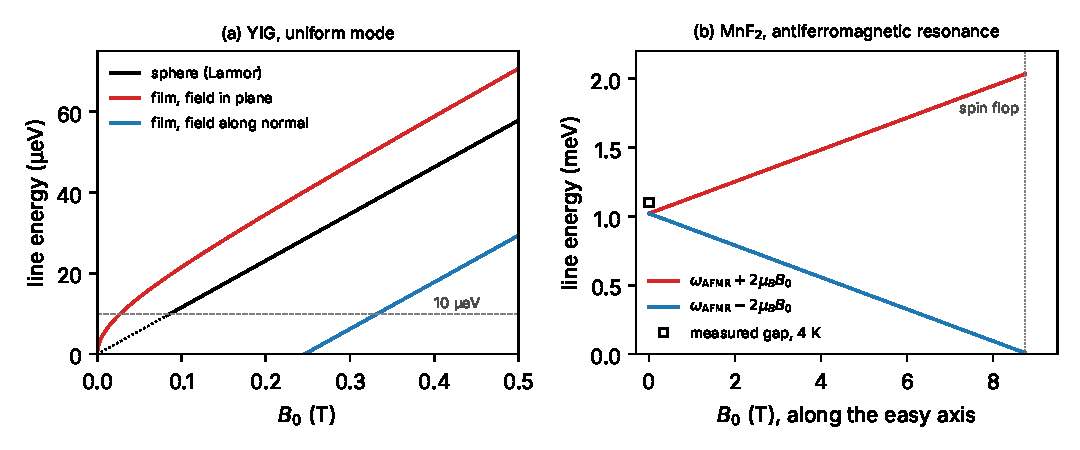
\includegraphics[width=0.95\linewidth]{figures/ch14/fig14_3.pdf}
  \caption{Absorption lines of YIG and MnF$_2$ against the applied field $B_0$. (a) The uniform mode of YIG ($g_{\mathrm{ion}} = 2$, $\mu_0M_{\mathrm{s}} = \SI{0.246}{T}$). A sphere absorbs at the Larmor frequency $2\mu_BB_0$ once it is saturated, $B_0 > \mu_0M_{\mathrm{s}}/3$ (dotted below). A thin film absorbs at $[\omega_{\mathrm{Lar}}(\omega_{\mathrm{Lar}} + \omega_M)]^{1/2}$ with the field in its plane and at $\omega_{\mathrm{Lar}} - \omega_M$ with the field along its normal, $\omega_M = \SI{28.5}{\micro eV}$. The dashed line marks the \SI{10}{\micro eV} of the worked example. (b) The two antiferromagnetic-resonance lines of MnF$_2$, $\omega_{\mathrm{AFMR}} \pm 2\mu_BB_0$ with $\omega_{\mathrm{AFMR}} = \SI{1.021}{meV}$ from $B_E = \SI{47.05}{T}$ and $B_A = \SI{0.82}{T}$, for a field along the easy axis up to the spin flop at \SI{8.75}{T}, both from the fitted fields; each line carries half of the weight $|\mathbf{S}|\omega_{\mathrm{AFMR}}/(2\omega_E + \omega_A) = 0.232$ per pair. The square is the measured zone-center gap at \SI{4}{K}, \SI{1.1}{meV}, which goes with a measured spin flop near \SI{9.4}{T}.}
  \label{fig:14-lines}
\end{figure}

\begin{limitbox}[Absorption into magnons][lim:14.3a]
(a) The Larmor statement: at $\vect{k} \to 0$ all transverse spin weight of a magnet with isotropic exchange and uniform $\lambda_S$ and $g_{\mathrm{ion}}$ lies in one line at $\omega_{\mathrm{Lar}}$ with weight $2\langle S^z_{\mathrm{tot}}\rangle$~\cites[Eqs.~(2.4), (2.5)]{oshikawa2002electron}[Eqs.~(25)--(27)]{chigusa2020detecting}[Eq.~(27)]{mitridate2020detectability}; for a $J$ multiplet the axion-like particle couples with $\lambda_S = g_J - 1$. (b) The uniform weight $|\vect{S}|\omega_{\mathrm{AFMR}}/(2\omega_E + \omega_A)$ per antiparallel pair, \cref{eq:14.3-afmrweight}.
\par\smallskip
{\centering
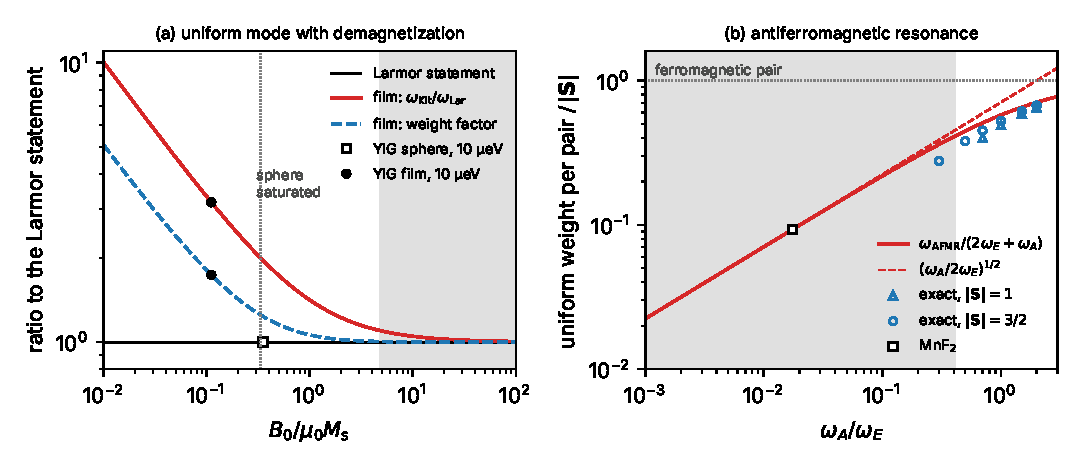
\includegraphics[width=0.98\linewidth]{figures/ch14/limit14_3a.pdf}
\captionof{figure}{(a) Uniform mode of a thin film with the field in its plane against the applied field over the shape-anisotropy field, $B_0/\mu_0M_{\mathrm{s}}$: line position $\omega_{\mathrm{Kit}}/\omega_{\mathrm{Lar}} = (1 + \mu_0M_{\mathrm{s}}/B_0)^{1/2}$ (solid) and weight averaged over transverse directions of $\vect{p}_\phi$ (dashed), both relative to the Larmor statement (black, 1). A saturated sphere follows the Larmor statement exactly; the markers place YIG at \SI{10}{\micro eV}. Gray: both ratios within \SI{10}{\percent} of 1, $B_0 \ge 4.8\,\mu_0M_{\mathrm{s}}$. For a $J$ multiplet both curves keep their shape, the rate scales by $(g_J - 1)^2$ and the line moves to $g_J\mu_BB_0$. (b) Uniform weight per antiparallel pair over $|\mathbf{S}|$ against $\omega_A/\omega_E$: the linear spin-wave result (solid) and its exchange-suppressed form $(\omega_A/2\omega_E)^{1/2}$ (dashed). Symbols: the exact total weight $\langle(S^x_{\mathrm{tot}})^2\rangle$ of the eight-site easy-axis (XXZ) cluster of the text for $|\mathbf{S}| = 1$ and $\frac32$, where that cluster is ordered (the splitting of its two lowest states below \SI{1}{\percent} of $\omega_{\mathrm{AFMR}}$). Gray: the square-root form within \SI{10}{\percent}, $\omega_A \le 0.42\,\omega_E$. The square marks MnF$_2$ with the fitted fields. The isotropic Heisenberg magnet, with zero uniform weight, is the left end.}\label{fig:14-limit-absorption}
\par}
\smallskip
Outside the gray regions the line of a non-spherical sample leaves $\omega_{\mathrm{Lar}}$ and its weight becomes elliptical, the antiferromagnetic weight departs from the square-root form, and in the eight-site cluster the zero-point fluctuations remove 5 to \SI{23}{\percent} of the linear spin-wave weight for $|\mathbf{S}| = \frac32$ ($\omega_A/\omega_E$ from 2 to 0.3).
\end{limitbox}

Linear spin-wave theory itself adds no correction to the Larmor line and one to the antiferromagnetic weight. \Cref{eq:14.3-larmor} is exact for any spin and temperature, and its only inputs are $\lambda_S$, $g_{\mathrm{ion}}$ and the net magnetization. The antiferromagnetic weight is of order $|\vect{S}|^0$ in the expansion of \cref{sec:14.1}, and an exactly solvable cluster shows its zero-point correction directly. Put spins $|\vect{S}|$ on the eight corners of a cube, each coupled to its three neighbors on the other sublattice by $H = J\sum_{\langle ij\rangle}(S^x_iS^x_j + S^y_iS^y_j + \Delta_{\mathrm{XXZ}}S^z_iS^z_j)$ with $J > 0$ and $\Delta_{\mathrm{XXZ}} \ge 1$, twelve bonds and open boundaries. Linear spin-wave theory at $\vect{k} = 0$ maps it onto \cref{eq:14.3-afmr} with $\omega_E = 3J|\vect{S}|$ and $\omega_A = 3J|\vect{S}|(\Delta_{\mathrm{XXZ}} - 1)$, so that \cref{eq:14.3-afmrweight} becomes $|\vect{S}|[(\Delta_{\mathrm{XXZ}} - 1)/(\Delta_{\mathrm{XXZ}} + 1)]^{1/2}$. The exact weight is the equal-time correlation $\langle0|(S^x_{\mathrm{tot}})^2|0\rangle$ in the ground state of the sector $S^z_{\mathrm{tot}} = 0$, divided by the four antiparallel pairs; it contains every final state that $S^x_{\mathrm{tot}}$ reaches. At $\omega_A = \omega_E$ it is 0.85 and 0.91 of \cref{eq:14.3-afmrweight} for $|\vect{S}| = 1$ and $\frac32$ (\cref{fig:14-limit-absorption}b). The cluster cannot reach the small anisotropies of real antiferromagnets, $\omega_A/\omega_E = 0.017$ in MnF$_2$, because below $\omega_A \approx 0.3\,\omega_E$ for $|\vect{S}| = \frac32$, and about $0.6\,\omega_E$ for $|\vect{S}| = 1$, its two lowest states mix and it no longer orders. For Mn$^{2+}$ the expansion parameter $1/2|\vect{S}|$ is 0.2, which sets the order of the correction at small $\omega_A/\omega_E$ but not its size.

\section{Spin responses from neutron data}\label{sec:14.4}

The full magnon spectrum of YIG, all twenty branches up to about \SI{110}{meV}, has been measured by inelastic neutron scattering with neutrons of \SI{120}{meV}~\cite{princep2017full,berlin2025determining}. Such a neutron carries \SI{15.0}{keV} of momentum, the largest momentum of a dark-matter particle of \SI{5.7}{MeV}, and its spin couples to the spin density $\vect{s}_e(\vect{q})$ (\cref{app:C.19}). The measured cross-section can therefore replace the model response of \cref{sec:14.1}, with every magnon branch, every multi-magnon process and the magnetic form factor already included, as Berlin, Millar, Trickle and Zhou did for YIG~\cite{berlin2025determining}. A neutron, however, couples only to the part of the spin density perpendicular to the momentum transfer, and how much of the dark-matter response that part fixes depends on the coupling and on how much model input is added for the magnet.

\subsection{Conversion of neutron spectra}

Neutron spectra are reported per formula unit of the crystal. With $N_{\mathrm{fu}}$ formula units in a cell of volume $\Omega$, the measured magnetic structure factor $S^{\mathrm{neu}}(\vect{q},\omega)$ is defined by $\dd^2\sigma/\dd\Omega\,\dd E' = (p'_n/p_n)\,S^{\mathrm{neu}}$ for one formula unit, with $\dd\Omega$ here the solid angle of the outgoing neutron. Dividing \cref{eq:C.19-cross} by the number of formula units in the sample, $\Vol N_{\mathrm{fu}}/\Omega$, and solving for the response,
\begin{equation}
  \Tr\bigl[P_T\,S(\vect{q},\omega)\bigr] = \sum_{a,b}(P_T)_{ab}\,S_{ab}(\vect{q},\omega) = \frac{2\pi N_{\mathrm{fu}}}{(\gamma_nr_{\mathrm{cl}})^2\,\Omega}\,S^{\mathrm{neu}}(\vect{q},\omega) ,
  \label{eq:14.4-PT}
\end{equation}
with $(P_T)_{ab} = \delta_{ab} - \hat q_a\hat q_b$ and $(\gamma_nr_{\mathrm{cl}})^2 = \SI{0.2906}{b}$. This is the relation of Berlin et al.~\cite[Eq.~(26)]{berlin2025determining}. The thermal vibration of the ions enters through the Debye--Waller factor, which the dark matter sees in the same way, so it stays inside $S_{ab}$ (\cref{app:C.19}).

Two corrections, for temperature and for the orbital moment, turn \cref{eq:14.4-PT} into the response that a detector needs. The spectrum is measured at a temperature $T_{\mathrm{d}}$, below \SI{10}{K} for the YIG data~\cite[App.~B\,2]{berlin2025determining}, while a detector runs at millikelvin. By the fluctuation--dissipation theorem \cref{eq:4.2-fdt}, $(1 - \ee^{-\beta\omega})S_{ab}$ is the dissipative response, and for free magnons this response does not depend on temperature, as for the thermal oscillator of \cref{sec:4.2}. Hence
\begin{equation*}
  S_{ab}(\vect{q},\omega;T \to 0) = \bigl(1 - \ee^{-\omega/T_{\mathrm{d}}}\bigr)\,S_{ab}(\vect{q},\omega;T_{\mathrm{d}}) , \qquad \omega > 0 ,
\end{equation*}
which removes the thermal population of the measured spectrum. The residual is set by the magnon interactions, which make the response follow the thermal reduction of the ordered moment; it is small for $T_{\mathrm{d}}$ well below the ordering temperature.

The second correction is the orbital moment. A neutron couples to the magnetization, spin and orbital, while spin-coupled dark matter couples to the spin alone. For a quenched $3d$ ion of spin $\vect{S}$, \cref{sec:14.3} showed that spin--orbit coupling induces an orbital moment $\vect{L} = (g_{\mathrm{ion}} - 2)\vect{S}$ at first order, with $g_{\mathrm{ion}}$ the spectroscopic $g$ factor of the ion (\cref{sec:14.3-lande}), taken isotropic here, while the spin itself changes only at second order, $\lambda_S = 1 - O(\xi_{\mathrm{ion}}^2/\Delta_{\mathrm{CF}}^2)$. In the dipole approximation of \cref{app:C.19} the spin part of the moment carries the radial integral $\langle j_0\rangle$ and the orbital part $\langle j_0\rangle + \langle j_2\rangle$. The moment $2\vect{S}\langle j_0\rangle + \vect{L}(\langle j_0\rangle + \langle j_2\rangle)$ is then $g_{\mathrm{ion}}\vect{S}\,F^{\mathrm{mag}}_g(q)$, and the neutron couples to
\begin{equation*}
  \vect{s}_e(\vect{q}) \to \frac{g_{\mathrm{ion}}}{2}\,F^{\mathrm{mag}}_g(q)\sum_j\ee^{\ii\vect{q}\cdot\vect{R}_j}\vect{S}_j, \qquad F^{\mathrm{mag}}_g(q) = \langle j_0(q)\rangle + \Bigl(1 - \frac2g\Bigr)\langle j_2(q)\rangle ,
\end{equation*}
while the dark matter couples to $\lambda_S\langle j_0(q)\rangle\sum_j\ee^{\ii\vect{q}\cdot\vect{R}_j}\vect{S}_j$. The two operators differ by a number at each $q$, so their responses differ by its square:
\begin{keyresult}[Data-driven spin response]
\begin{equation}
  \Tr\bigl[P_T\,S(\vect{q},\omega)\bigr] = C_{\mathrm{sn}}(q)\,\frac{2\pi N_{\mathrm{fu}}}{(\gamma_nr_{\mathrm{cl}})^2\,\Omega}\,S^{\mathrm{neu}}(\vect{q},\omega), \qquad
  C_{\mathrm{sn}}(q) = \biggl[\frac{\lambda_S\,\langle j_0(q)\rangle}{(g_{\mathrm{ion}}/2)\,F^{\mathrm{mag}}_g(q)}\biggr]^2 ,
  \label{eq:14.4-data}
\end{equation}
for one species of quenched magnetic ion, with $S_{ab}$ the response of the electron spin density and $S^{\mathrm{neu}}$ measured per formula unit, its thermal population removed. At $q \to 0$, $C_{\mathrm{sn}} = [\lambda_S/(g_{\mathrm{ion}}/2)]^2$.
\end{keyresult}
\noindent For an anisotropic $g_{\mathrm{ion}}$ tensor, $g_{\mathrm{ion}}/2$ becomes the matrix $g_{\mathrm{ion},ab}/2$ acting on both indices of $S_{ab}$. For a $J$ multiplet, $g_{\mathrm{ion}}$ is replaced by $g_J$, $\lambda_S$ by $g_J - 1$ (\cref{eq:14.3-gJ}) and $F^{\mathrm{mag}}_g$ by the dipole form factor \cref{eq:C.19-dipole}; at $q \to 0$, $C_{\mathrm{sn}}$ is the square of the last column of \cref{tab:14-lande}. It is 1 for Gd$^{3+}$, $\frac19$ for Er$^{3+}$ and 25 for Sm$^{3+}$, whose spin points against its moment.

For Ni$^{2+}$ in NiO, $g_{\mathrm{ion}} = 2.18 \simeq 2.2$~\cite{kritzell2024terahertz}. With $\lambda_S = 1$,
\begin{equation*}
  C_{\mathrm{sn}}(0) = \Bigl(\frac{2}{2.2}\Bigr)^2 = 0.83 :
\end{equation*}
the spin response of NiO is \SI{17}{\percent} below what the neutron cross-section suggests if read as pure spin. Setting $\lambda_S = g_{\mathrm{ion}} - 1$ instead, the rule that holds only for $J$ multiplets, would give $(1.2/1.1)^2 = 1.19$ and an error of the opposite sign. The $q$ dependence enters through $\langle j_2\rangle$, which vanishes at $q = 0$ and grows with $q$. With the tabulated radial integrals of Ni$^{2+}$~\cite[Sect.~4.4.5]{anderson2006neutron}, the same fit form as for $\langle j_0\rangle$ in \cref{sec:14.1} multiplied by $s^2$ with coefficients $(1.708, 11.016, 1.2147, 4.103, 0.315, 1.533, 0.0018)$, the ratio $\langle j_2\rangle/\langle j_0\rangle$ is 0.035 at $|\vect{Q}_{\mathrm{AF}}| = \SI{2.6}{keV}$ and 0.15 at \SI{5.3}{keV}. $C_{\mathrm{sn}}(q)/C_{\mathrm{sn}}(0)$ is then 0.994 and 0.973, and it stays within \SI{10}{\percent} of one up to \SI{10}{keV}. The value of $g_{\mathrm{ion}}$ is the larger uncertainty. Magnetic x-ray diffraction on NiO, which separates the spin and orbital moments, finds $L/S = 0.34$~\cite{fernandez1998observation}, and DFT~$+\,U$ with spin--orbit coupling gives 0.36~\cite{kwon2000unquenched}. Read in the quenched picture as $g_{\mathrm{ion}} = 2 + L/S = 2.34$, this lowers $C_{\mathrm{sn}}(0)$ to 0.73, \SI{12}{\percent} below the value at $g_{\mathrm{ion}} = 2.2$. The orbital moment of Ni$^{2+}$ is thus an uncertainty of about \SI{10}{\percent} on the normalization of the data-driven rate. The $g_{\mathrm{ion}}$ tensor and the orbital moments are computed in DFT~$+\,U$ with spin--orbit coupling (\cref{app:E.20-magnet}), and the radial integrals from Dirac--Fock or Wannier-projected shells.

\Cref{lim:14.4a} shows how far the spin-only reading of the data holds as the orbital admixture grows.
\begin{limitbox}[Data-driven spin response][lim:14.4a]
$\Tr[P_TS(\vect{q},\omega)] = 2\pi N_{\mathrm{fu}}S^{\mathrm{neu}}(\vect{q},\omega)/[(\gamma_nr_{\mathrm{cl}})^2\Omega]$, for a neutron coupled to the electron spin alone~\cite[Eqs.~(8), (11), (26)]{berlin2025determining}.
\par\smallskip
{\centering
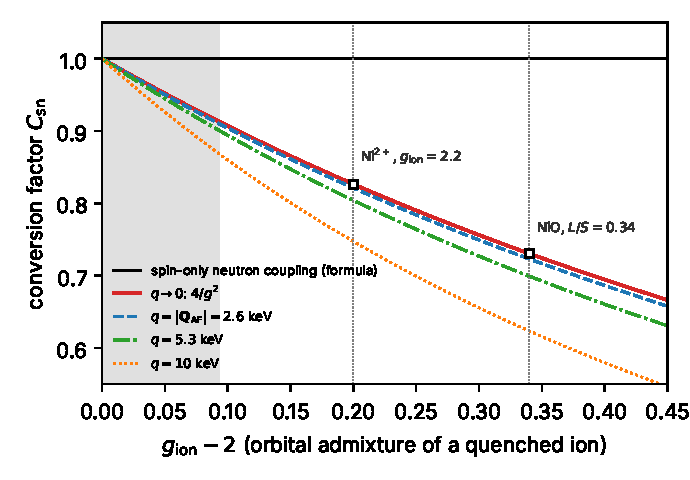
\includegraphics[width=0.78\linewidth]{figures/ch14/limit14_4a.pdf}
\captionof{figure}{Ratio of the spin response to the response inferred from neutron data by the spin-only formula, $C_{\mathrm{sn}}(q)$ of \cref{eq:14.4-data}, against the shift $g_{\mathrm{ion}} - 2$ of the spectroscopic $g_{\mathrm{ion}}$ factor of a quenched ion, with $\lambda_S = 1$ and the dipole form factor $\langle j_0\rangle + (1 - 2/g_{\mathrm{ion}})\langle j_2\rangle$. Black: the formula, ratio 1. Red: $q \to 0$, $4/g^2$. Dashed, dash-dotted and dotted: $q = \SI{2.6}{keV}$ (the ordering wavevector of NiO), \SI{5.3}{keV} (largest momentum transfer at $\mchi = \SI{1}{MeV}$) and \SI{10}{keV}, with the radial integrals of Ni$^{2+}$. Squares: $g_{\mathrm{ion}} = 2.2$ (octahedral Ni$^{2+}$) and $g_{\mathrm{ion}} = 2.34$ (NiO with $L/S = 0.34$ from magnetic x-ray diffraction). Gray: $g_{\mathrm{ion}} - 2 \le 0.094$, where the formula holds within \SI{10}{\percent} for $q \le \SI{5.3}{keV}$.}\label{fig:14-limit-neutron}
\par}
\smallskip
Outside the gray band the orbital moment shifts the neutron response from the spin response at first order in $g_{\mathrm{ion}} - 2$, and at large $q$ the orbital form factor $\langle j_2\rangle$ adds to the shift.
\end{limitbox}

How much of the dark-matter kinematic region the data reach depends on the instrument. In the YIG spectrum of Berlin et al.\ the data below \SI{5}{meV} are dominated by elastic scattering and are discarded, and the crystal was rotated about one axis only, so at large $q$ only a narrow band of directions $\hat{\vect{q}}$ is covered~\cite[Sect.~III\,B and App.~D]{berlin2025determining}. Averaging $S^{\mathrm{neu}}$ over the covered directions at fixed $|\vect{q}|$ and $\omega$ is justified well outside the first zone, since a small change in the direction of $\vect{q}$ moves its reduced part across the whole zone. Below a mass of \SI{134}{keV}, where $2\mchi v_{\mathrm{max}}$ reaches the radius $\sqrt2\pi/a = \SI{708}{eV}$ of the largest sphere inside the zone, every momentum transfer lies inside the first zone, where there are few data, and the data-driven reach falls rapidly below about \SI{200}{keV}. Near \SI{1}{MeV} the data-driven rate agrees closely with the Heisenberg-model rate fitted to the same spectrum~\cite[Fig.~3]{berlin2025determining}. At larger masses the data contain the form factor of Fe$^{3+}$, which the model omits and which suppresses the rate by an order of magnitude for $q \gtrsim \SI{10}{keV}$. They also contain phonons, excited by the nuclear scattering of the neutron with a relative weight that grows as $q^2/(M\omega)$, about $(q/\SI{30}{keV})^2$ for nuclei of \SI{50}{GeV} and $\omega \sim \SI{20}{meV}$~\cite[App.~C]{berlin2025determining}. Spin-flip scattering with the polarization along $\hat{\vect{q}}$ contains all the magnetic scattering and no coherent nuclear scattering (\cref{app:C.19}), and it removes the phonons without a model, up to the two thirds of the nuclear-spin-incoherent scattering that it keeps, which is small for Y, Fe and O. A modelled phonon part subtracted from unpolarized data must leave a response that is still positive semidefinite (\cref{eq:4.2-positivity}).

\subsection{Transverse projection of the neutron cross-section}

Which couplings \cref{eq:14.4-PT} calibrates depends on the dark-matter tensor $\mathfrak{D}_{ab}$ of \cref{eq:8.1-D} for the spin row. For the operators of \cref{tab:8-operators} with dark matter of spin $\frac12$ there are three structures. The contact interaction $\mathcal{O}_4$ gives $\mathfrak{D}_{ab} = |c_4^{(e)}|^2\delta_{ab}/4$. The pseudoscalar couplings give $\hat q_a\hat q_b$: $\mathcal{O}_{10}$ gives $|c_{10}^{(e)}|^2q_aq_b/m_e^2$ and $\mathcal{O}_6$ gives $|c_6^{(e)}|^2q^2q_aq_b/4m_e^4$. Operator $\mathcal{O}_9 = \ii\vect{S}_\chi\cdot(\vect{S}_e\times\vect{q}/m_e)$, and the spin--spin part $(\vect{S}_\chi\times\vect{q})\cdot(\vect{S}_e\times\vect{q})$ of magnetic-dipole and anapole dark matter, give the transverse projector: for $\mathcal{O}_9$, $\Tr_\chi[(\vect{q}\times\vect{S}_\chi)_a(\vect{q}\times\vect{S}_\chi)_b]/2 = q^2(P_T)_{ab}/4$, so $\mathfrak{D}_{ab} = |c_9^{(e)}|^2q^2(P_T)_{ab}/4m_e^2$. Since $\delta_{ab} = (P_T)_{ab} + \hat q_a\hat q_b$, the three contractions are
\begin{equation}
  \sum_{a,b}\delta_{ab}S_{ab} = \Tr\bigl[P_TS\bigr] + \hat{\vect{q}}\cdot S\cdot\hat{\vect{q}}, \qquad \sum_{a,b}(P_T)_{ab}S_{ab} = \Tr\bigl[P_TS\bigr], \qquad \sum_{a,b}\hat q_a\hat q_bS_{ab} = \hat{\vect{q}}\cdot S\cdot\hat{\vect{q}} .
  \label{eq:14.4-split}
\end{equation}
The neutron data fix the transverse couplings completely: the rates of $\mathcal{O}_9$, magnetic-dipole and anapole dark matter follow from \cref{eq:8.2-spectrum} with $S^{\mathrm{neu}}$ and nothing else. For $\mathcal{O}_4$, however, the transverse part alone is only a lower bound on the rate of the contact interaction: the longitudinal element $\hat{\vect{q}}\cdot S\cdot\hat{\vect{q}}$ is a diagonal element of a positive semidefinite matrix and cannot be negative. For $\mathcal{O}_6$ and $\mathcal{O}_{10}$ the data at one $\vect{q}$ leave the rate unconstrained. Tensors built from the dark-matter velocity, as for $\mathcal{O}_7$ and $\mathcal{O}_{12}$--$\mathcal{O}_{15}$, also need the mixed elements between the direction of $\vect{q}$ and the two directions perpendicular to it.

Absorption needs exactly the missing element. The spin row of an axion-like particle is proportional to its momentum, and the absorption rate \cref{eq:14.3-abs} contracts $S_{ab}$ with $p_{\phi,a}p_{\phi,b}$: it is $p_\phi^2\,\hat{\vect{p}}_\phi\cdot S\cdot\hat{\vect{p}}_\phi$, a longitudinal element~\cite[Eqs.~(15), (17)]{berlin2025determining}. Its momentum, $p_\phi \sim 10^{-3}m_\phi$, is also far below any momentum transfer a neutron spectrometer resolves. At $q \to 0$ the full tensor is fixed instead by the magnetic permeability measured in resonance or terahertz experiments~\cite[footnote~3]{berlin2025determining}, and in the model of \cref{sec:14.3} by the Larmor and Kittel lines.

That the longitudinal element is missing at each $q$, whatever the beam, follows from the form of the amplitude. \Cref{fig:14-neutron} shows the geometry.
\begin{keyresult}[Neutron scattering and the longitudinal spin response]
At a given $\vect{q}$, magnetic neutron scattering measures only the block of $S_{ab}(\vect{q},\omega)$ transverse to $\hat{\vect{q}}$: unpolarized beams its trace $\Tr[P_TS]$, polarization analysis its elements. Without a model of the magnet (of the spin density within the cell, or the spin-isotropy hypothesis of \cref{sec:14.4-iso}), the longitudinal element $\hat{\vect{q}}\cdot S\cdot\hat{\vect{q}}$ and the mixed elements between $\hat{\vect{q}}$ and the transverse plane are measured by no neutron experiment, polarized or not, and no symmetry of the crystal relates them to the transverse block at the same $\vect{q}$. Within the localized-moment model of \cref{eq:14.4-data}, transverse data at several wavevectors $\vect{q} + \vect{G}$ determine the full tensor.
\end{keyresult}
\noindent The first part is the perpendicular-projection rule of magnetic neutron scattering (\cref{app:C.19}). Every amplitude in \cref{eq:C.19-amplitude,eq:C.19-polar} contains $\vect{s}_e$ only through $\vect{s}_\perp = P_T\vect{s}_e$, because a spin density modulated along $\vect{q}$ produces no magnetic field at that wavevector (\cref{eq:C.19-field}). In the frame of \cref{app:C.19}, with $x$ along $\hat{\vect{q}}$, polarization analysis separates $S_{yy}$, $S_{zz}$ and the chiral part of $S_{yz}$, and full polarimetry reaches its symmetric part as well~\cite{blume1963polarization}. That is at most four of the nine real numbers of the Hermitian matrix $S_{ab}$.

For the second part, let $\mathsf{h}$ be an element of the magnetic point group, acting as a rotation matrix $\mathsf{R}$ on positions and on the axial spin. It maps the response at $\vect{q}$ onto the response at $\mathsf{R}\vect{q}$, $S(\mathsf{R}\vect{q}) = \mathsf{R}\,S(\vect{q})\,\mathsf{R}^{\mathrm{T}}$, possibly transposed if $\mathsf{h}$ contains time reversal; the transpose does not change the symmetric contractions. Since also $P_T(\mathsf{R}\hat{\vect{q}}) = \mathsf{R}\,P_T(\hat{\vect{q}})\,\mathsf{R}^{\mathrm{T}}$,
\begin{equation*}
  \Tr\bigl[P_T(\mathsf{R}\hat{\vect{q}})\,S(\mathsf{R}\vect{q})\bigr] = \Tr\bigl[\mathsf{R}P_T(\hat{\vect{q}})\mathsf{R}^{\mathrm{T}}\mathsf{R}S(\vect{q})\mathsf{R}^{\mathrm{T}}\bigr] = \Tr\bigl[P_T(\hat{\vect{q}})\,S(\vect{q})\bigr] ,
\end{equation*}
and a measurement at a symmetry-equivalent wavevector repeats the same equation. The elements that leave $\hat{\vect{q}}$ fixed map the direction of $\vect{q}$ onto itself and the transverse plane onto itself, so they constrain the transverse block and the longitudinal element separately and never relate one to the other. A wavevector $\vect{q} + \vect{G}$ that points elsewhere belongs to a different operator, $\vect{s}_e(\vect{q} + \vect{G})$, which the exact response does not tie to $\vect{s}_e(\vect{q})$.

The localized-moment form that \cref{eq:14.4-data} already uses supplies that tie. For one magnetic ion per primitive cell, as for NiO in its chemical cell, $\vect{s}_e(\vect{k} + \vect{G}) = F^{\mathrm{mag}}(|\vect{k} + \vect{G}|)\sum_j\ee^{\ii(\vect{k}+\vect{G})\cdot\vect{R}_j}\vect{S}_j$ with $\ee^{\ii\vect{G}\cdot\vect{R}_j} = 1$, so that
\begin{equation}
  S_{ab}(\vect{k} + \vect{G},\omega) = |F^{\mathrm{mag}}(|\vect{k} + \vect{G}|)|^2\,\ee^{-2W(\vect{k}+\vect{G})}\,S^{\mathrm{lat}}_{ab}(\vect{k},\omega) ,
  \label{eq:14.4-Glat}
\end{equation}
for every reciprocal vector $\vect{G}$, with $S^{\mathrm{lat}}$ the response of the lattice spins and the Debye--Waller factor $\ee^{-2W}$ taken at $\vect{k} + \vect{G}$, beside the form factor. Each $\vect{G}$ gives the transverse trace $\Tr S^{\mathrm{lat}} - \hat{\vect{n}}_{\vect{G}}\cdot S^{\mathrm{lat}}\cdot\hat{\vect{n}}_{\vect{G}}$ along its own direction $\hat{\vect{n}}_{\vect{G}} = (\vect{k} + \vect{G})/|\vect{k} + \vect{G}|$, a linear equation for the six components of the symmetric part of $S^{\mathrm{lat}}(\vect{k},\omega)$, and six generic directions fix all six. For NiO the four shortest vectors of type $(111)$ and two of type $(200)$ already give a system of full rank. The longitudinal element at the momentum transfer of the dark matter then follows from \cref{eq:14.4-Glat}, and as $\vect{k} \to 0$ so does the tensor that absorption needs, resolution permitting; neutron diffraction fixes the directions of ordered moments in the same way. The route rests on the dipole-approximation form factor, which gives every spin component the same radial shape, and on a known magnetic basis; with several magnetic ions per cell, as in YIG, the phases $\ee^{\ii\vect{G}\cdot\vect{\tau}}$ of the basis enter and more wavevectors are needed.

\begin{figure}[tbp]
  \centering
  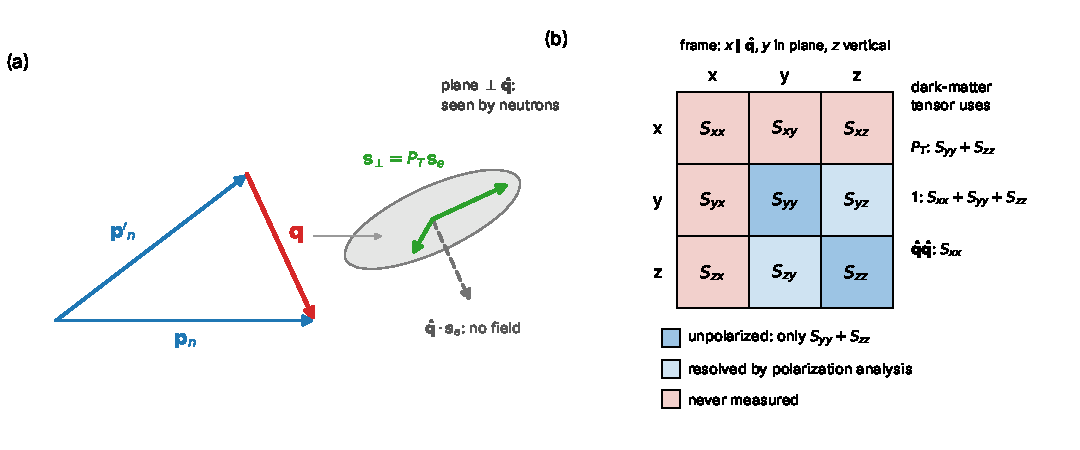
\includegraphics[width=\linewidth]{figures/ch14/fig14_4.pdf}
  \caption{The neutron geometry and the transverse projector. (a) A neutron of momentum $\mathbf{p}_n$ leaves with $\mathbf{p}'_n$ and gives the target $\vect{q} = \mathbf{p}_n - \mathbf{p}'_n$. Of the spin density at wavevector $\vect{q}$, only the part in the plane perpendicular to $\hat{\vect{q}}$, $\vect{s}_\perp = P_T\vect{s}_e$, produces a magnetic field and scatters the neutron; the component along $\hat{\vect{q}}$ produces none. (b) The spin response $S_{ab}$ in the frame with $x$ along $\hat{\vect{q}}$, $y$ in the scattering plane and $z$ vertical. Unpolarized neutrons measure the sum $S_{yy} + S_{zz}$; polarization analysis resolves the transverse block; the elements in the first row and column are not measured at this $\vect{q}$. Right-hand columns of (b): the elements that the dark-matter tensors proportional to $P_T$ (for example $\mathcal{O}_9$), to the unit matrix ($\mathcal{O}_4$) and to $\hat q_a\hat q_b$ ($\mathcal{O}_6$, $\mathcal{O}_{10}$) contract. Schematic.}
  \label{fig:14-neutron}
\end{figure}

\subsection{The longitudinal response under isotropy}\label{sec:14.4-iso}

Spin-rotation symmetry about the moments supplies the missing element at one $\vect{q}$, without a model of the spin density but with a hypothesis on the Hamiltonian: spin--orbit coupling and the dipolar interaction are neglected. In a collinear magnet with moments along $\pm\hat{\vect{m}}$, and with spin--orbit coupling neglected, the Hamiltonian is invariant under rotations of all spins about $\hat{\vect{m}}$, independently of the lattice; the Heisenberg model of \cref{sec:7.1} is the example. A rotation of the spin indices alone then leaves $S_{ab}(\vect{q},\omega)$ unchanged at every $\vect{q}$, and the only tensors with that property are built from $\delta_{ab}$, $\hat m_a\hat m_b$ and $\epsilon_{abc}\hat m_c$:
\begin{equation*}
  S_{ab}(\vect{q},\omega) = S_\parallel\,\hat m_a\hat m_b + S_\perp\,(\delta_{ab} - \hat m_a\hat m_b) + \ii S_{\mathrm{c}}\,\epsilon_{abc}\hat m_c ,
\end{equation*}
with three functions of $\vect{q}$ and $\omega$. The one-magnon response \cref{eq:14.1-Safm} has this form with $S_\parallel = 0$, and the two-magnon response \cref{eq:14.2-S2m} is all $S_\parallel$. The antisymmetric part drops out of every symmetric contraction. With $\theta_m$ the angle between $\hat{\vect{q}}$ and $\hat{\vect{m}}$,
\begin{equation}
  \Tr\bigl[P_TS\bigr] = S_\parallel\sin^2\theta_m + S_\perp(1 + \cos^2\theta_m), \qquad
  \hat{\vect{q}}\cdot S\cdot\hat{\vect{q}} = S_\parallel\cos^2\theta_m + S_\perp\sin^2\theta_m .
  \label{eq:14.4-uniax}
\end{equation}
Polarization analysis now suffices at a single $\vect{q}$. With $\hat{\vect{m}}$ in the scattering plane at an angle $\theta_m \ne 0, \frac\pi2$ to $\hat{\vect{q}}$, the vertical element is $S_{zz} = S_\perp$ and the in-plane element $S_{yy} = S_\parallel\sin^2\theta_m + S_\perp\cos^2\theta_m$, which equals $\hat{\vect{q}}\cdot S\cdot\hat{\vect{q}}$ with $\cos$ and $\sin$ exchanged and fixes $S_\parallel$. Unpolarized data give one equation for two unknowns at each $\vect{q}$, and a second measurement is needed at another angle with the same $S_\parallel$ and $S_\perp$. That is the content of the \emph{isotropy hypothesis}: in the window used, $S_\parallel$ and $S_\perp$ depend on $\vect{q}$ only through $|\vect{q}|$, or do not change when the moments are turned at fixed $\vect{q}$. The second form is the easier one to realize. A soft magnet can be turned by an applied field with $\vect{q}$ held fixed in the crystal; a YIG sphere saturates above \SI{82}{mT} (\cref{we:14-yig}). In the spin-rotation-invariant model the two settings then measure exactly the same $S_\parallel$ and $S_\perp$, and only spin--orbit coupling and the magnetic dipolar interaction break the hypothesis. The dipolar term, $\omega_M\sin^2\theta_{\vect{q}}$ in the spin-wave energy with $\omega_M = \SI{28.5}{\micro eV}$ for YIG (\cref{we:14-yig}), is negligible above about \SI{0.1}{meV}, far below the \SI{5}{meV} where the data start. Given $P_i = \Tr[P_TS]$ at two angles $\theta_1$ and $\theta_2$, with $c_i = \cos^2\theta_i$, the solution of the two equations \cref{eq:14.4-uniax} is
\begin{equation}
  S_\parallel = \frac{P_1(1 + c_2) - P_2(1 + c_1)}{2(c_2 - c_1)}, \qquad S_\perp = \frac{P_2(1 - c_1) - P_1(1 - c_2)}{2(c_2 - c_1)} ,
  \label{eq:14.4-invert}
\end{equation}
and the longitudinal element follows from \cref{eq:14.4-uniax} for any direction of $\vect{q}$ relative to $\hat{\vect{m}}$.

A paramagnet in zero field, or a sample of many randomly oriented domains, is invariant under all rotations, so $S_\parallel = S_\perp$ and $\hat{\vect{q}}\cdot S\cdot\hat{\vect{q}} = \frac12\Tr[P_TS]$~\cite[Eq.~(35)]{berlin2025determining}. In an ordered magnet the two-magnon continuum, \SI{7.3}{\percent} of the one-magnon weight in NiO (\cref{we:14-nio}), lies entirely in $S_\parallel$, and the two-angle inversion keeps it.

\begin{workedexample}{The two-angle inversion for an isotropic paramagnet}\label{we:14-paramagnet}
Take a paramagnet in zero field, so that $S_\parallel = S_\perp = S_0$ at the $(|\vect{q}|, \omega)$ of interest, and measure $\Tr[P_TS]$ with $\vect{q}$ perpendicular and then parallel to a fixed crystal axis $\hat{\vect{m}}$: $c_1 = 0$, $c_2 = 1$. Both measurements give $2S_0$, and \cref{eq:14.4-invert} reduces to $S_\parallel = P_1 - P_2/2$ and $S_\perp = P_2/2$, which returns $S_0$ for both. The hypothesis is tested by the data themselves: $P_2 - P_1 = (c_2 - c_1)(S_\perp - S_\parallel)$ vanishes.

Errors decide whether the inversion is worth doing. Give each measurement a statistical error of \SI{5}{\percent}, $0.1S_0$, independent between the two. Then $S_\perp$ carries $0.050S_0$, while $S_\parallel$ carries $(\sqrt5/2)\times0.1S_0 = 0.112S_0$, more than twice the relative error of the data. The longitudinal element needed for $\mathcal{O}_6$ along $\hat{\vect{m}}$ is $S_\parallel$ itself, with the same \SI{11}{\percent}; at $\cos^2\theta = \frac13$ it is $P_1/3 + P_2/6$, with \SI{3.7}{\percent}. The isotropy test, $P_2 - P_1 = 0 \pm 0.141S_0$, limits $|S_\perp - S_\parallel|$ to about \SI{14}{\percent} of $S_0$ at one standard deviation.

A smaller rotation gives larger errors. With $c_2 = \sin^2 30^\circ = 0.25$ instead, the denominator $2(c_2 - c_1)$ drops from 2 to 0.5, $S_\parallel = 2.5P_1 - 2P_2$ and its error grows to $0.32S_0$, \SI{32}{\percent}. The one-angle shortcut $\frac12\Tr[P_TS]$ has the \SI{5}{\percent} of the data, but it is right only if the paramagnet is in fact isotropic, which the two-angle measurement checks.
\end{workedexample}

A spin-wave model fitted to the transverse data supplies the longitudinal element as well, and its fit uncertainty enters as a normalization (\cref{sec:8.8}); a longitudinal response measured at dark-matter momenta, without such a model or the localized-moment form, does not exist.

\section{Coherent fields and precessing nuclear spins}\label{sec:14.6}

An axion-like field of mass \SI{1}{neV} oscillates at \SI{241.8}{kHz}, and its phase wanders on a time of about a second. A $^{207}$Pb nucleus in a field of \SI{26.8}{mT} precesses at the same frequency. Over a record shorter than a second the field acts on the nuclear spins as one classical wave with a fixed amplitude and phase, the spins tip together, and their transverse magnetization grows in proportion to the time until the spin coherence time $T_2$ caps it, after \SI{17}{ms} in the ferroelectric PMN-PT. The amplitude of the field then changes only on the scale of a second. Whether the golden-rule rate describes such a record depends on the shorter of the two times, and how the sensitivity of a search grows with the length of the record depends on the statistics of the random amplitude.

\subsection{The coherent classical-field regime}\label{sec:14.6-regime}

A light boson of mass $m_\phi$ has about $\rho_\chi/(m_\phi^4v_0^3)$ quanta in a volume $(1/m_\phi v_0)^3$, $4.6\times10^{39}$ at \SI{1}{neV}, and below a few eV it is a classical field (\cref{sec:8.2-absorption}). It is a sum of modes with random phases, one for each velocity in the halo, and by the central limit theorem a Gaussian random field~\cite[Eqs.~(3)--(10)]{foster2018revealing}. A Gaussian field with zero mean is fixed by its two-point function. For a free nonrelativistic field with the velocity distribution $f_\chi(\vect{v})$ of \cref{sec:1.2}, each mode oscillates at $\omega_{\vect{v}} = m_\phi(1 + v^2/2)$, and the average over the random phases is
\begin{equation*}
  \langle\phi(\vect{x},t)\,\phi(\vect{x}',t')\rangle = \frac{\rho_\chi}{m_\phi^2}\int\dd^3v\,f_\chi(\vect{v})\cos\bigl[\omega_{\vect{v}}(t - t') - m_\phi\vect{v}\cdot(\vect{x} - \vect{x}')\bigr] ,
\end{equation*}
normalized so that $\langle\phi^2\rangle = \rho_\chi/m_\phi^2$, the mean square of a wave $\phi_0\cos(m_\phi t)$ with $\tfrac12m_\phi^2\phi_0^2 = \rho_\chi$. With the transforms of \cref{app:A.3} in space and time, the power spectrum of the field is
\begin{equation}
  \mathcal{S}_\phi(\vect{k},\omega) = \frac{\pi\rho_\chi}{m_\phi^2}\,(2\pi)^3\!\int\dd^3v\,f_\chi(\vect{v})\Bigl[\delta^3(\vect{k} + m_\phi\vect{v})\,\delta(\omega - \omega_{\vect{v}}) + \delta^3(\vect{k} - m_\phi\vect{v})\,\delta(\omega + \omega_{\vect{v}})\Bigr] .
  \label{eq:14.6-Sphi}
\end{equation}
The positive-frequency weight sits at $\vect{k} = -m_\phi\vect{v}$ in the sign convention of \cref{eq:A.3-space,eq:A.3-time}, while the target receives the momentum $\vect{p}_\phi = m_\phi\vect{v}$, as in \cref{eq:8.2-abs}; the sign matters only for targets whose response is odd in $\vect{q}$ (\cref{sec:14.5}). Integrated over $\vect{k}$, the positive-frequency part is $(\pi\rho_\chi/m_\phi^2)F_\phi(\omega)$, with
\begin{equation}
  F_\phi(\omega)\,\dd\omega = F_\chi(v)\,\dd v, \qquad \omega - m_\phi = \tfrac12m_\phi v^2 ,
  \label{eq:14.6-Fphi}
\end{equation}
the energy distribution of the field of \cref{sec:11.8}, normalized to one and inherited from the laboratory speed distribution $F_\chi$ of \cref{sec:1.2}. The line is one-sided: it starts at $m_\phi$ and ends at $m_\phi(1 + v_{\mathrm{max}}^2/2)$, $3.5\times10^{-6}$ above it.

The width of the line sets the coherence time. We define it, as \cref{sec:8.2-absorption} estimated it, by
\begin{equation}
  t_{\mathrm{coh}} = \frac{1}{m_\phi v_0^2} = \SI{1.04}{s}\times\frac{\SI{1}{neV}}{m_\phi} ,
  \label{eq:14.6-tcoh}
\end{equation}
with $v_0 = \SI{238}{km/s}$. For the halo of \cref{sec:1.2} seen from the Earth, $F_\phi$ peaks at $0.58/t_{\mathrm{coh}}$ above $m_\phi$, its equivalent width $\Delta\omega_{\mathrm{eq}} = [\int\dd\omega\,F_\phi^2]^{-1}$ is $2.67/t_{\mathrm{coh}}$, and the correlation of the complex amplitude of the field with itself, $|\int\dd\omega\,F_\phi(\omega)\,\ee^{-\ii\omega t}|$, falls to one half at $t = 1.47\,t_{\mathrm{coh}}$. Over the coherence length $1/m_\phi v_0$, \SI{249}{km} at \SI{1}{neV}, the field is uniform, and every laboratory sample sees the same amplitude.

A coupling $\sum_bg^\phi_bO_b$ of the absorption rows of \cref{sec:8.1-absorption} drives the expectation value of any readout operator $O_{\mathrm{rd}}$ through the Kubo formula \cref{eq:4.1-kubo}, with the retarded response $R_{\mathrm{rd},b}(\vect{p}_\phi,t)$. The readout can be the operator that the field couples to, as for the magnetization of the spins below, or another, as for the voltage across a piezoelectric resonator (\cref{sec:11.8}). Either way the signal is linear in the amplitude of the field and in the coupling. Its square averaged over the Gaussian ensemble is quadratic in both and contains $\mathcal{S}_\phi$. The energy that the target absorbs is the case $O_{\mathrm{rd}} = \sum_bg^\phi_bO_b$, and its average reproduces the golden rule, but only after a long enough record. Take the coupling on from $t' = 0$ to $t$. The amplitude of a transition $i \to f$ driven by one mode of frequency $\omega$ contains $\int_0^t\dd t'\,\ee^{\ii(E_f - E_i - \omega)t'}$, whose square is $2\pi t\,\mathcal{K}_t(\omega - E_f + E_i)$ with the Fejér kernel
\begin{equation}
  \mathcal{K}_t(x) = \frac{t}{2\pi}\,\frac{\sin^2(xt/2)}{(xt/2)^2}, \qquad \int\dd x\,\mathcal{K}_t(x) = 1 .
  \label{eq:14.6-fejer}
\end{equation}
The Gaussian average removes the cross terms between modes, as in \cref{app:D.25}, and the mean number of quanta absorbed per unit volume in the record is $t\,(\rho_\chi/m_\phi)$ times the rate \cref{eq:8.2-abs} averaged over the line $F_\phi$, with the $\delta(\omega - E_f + E_i)$ in $S_{ab}$ replaced by $\mathcal{K}_t$. As $t \to \infty$ the kernel becomes the delta function and the mean is the golden-rule rate times $t$. The replacement matters only where both the field line and the target line are narrow compared with $1/t$. Since the kernel acts on their convolution, whose width is at least the larger of the two widths, the golden-rule mean holds for
\begin{equation*}
  t \gg \min\bigl(t_{\mathrm{coh}},\,1/\varGamma_{\mathrm{tg}}\bigr) .
\end{equation*}
Here $\varGamma_{\mathrm{tg}}$ is the width of the target's line: $1/T_2$ for nuclear spins, the full width $\varGamma_{\mathrm{M}}$ of a magnon line (\cref{sec:14.3}), $\gamma_n$ for a resonator mode (\cref{sec:11.8}). For a record shorter than both, the energy absorbed grows as $t^2$. That is the regime of a nuclear spin driven by a field of neV mass over a record shorter than its $T_2$, the coherent regime that \cref{sec:8.2-absorption} named.

The golden-rule mean is not yet what one record measures. A single realization of the field matches the ensemble only when the record spans many coherence times, so that it samples many independent amplitudes. For a detector that counts absorbed quanta, the intensity $|\Phi|^2$ of the complex amplitude $\Phi$ of the field is exponentially distributed within one coherence time, and a record of $N_{\mathrm{coh}}$ independent coherence times gives $\mathrm{Var}\,N = \bar N + \bar N^2/N_{\mathrm{coh}}$, the bunching of chaotic light. The Poisson statistics of \cref{eq:1.5-poisson} hold when $N_{\mathrm{coh}} \gg \bar N$, which counting searches satisfy by a wide margin: the YIG search of \cref{we:14-yig} at \SI{10}{\micro eV} sees 35 events per hour in $3.4\times10^7$ coherence times. A readout of the mean field, such as the magnetization below, is a different matter, since its signal is proportional to the amplitude of the field rather than to its intensity.

\subsection{Bloch equations and nuclear magnetic resonance}\label{sec:14.6-bloch}

A nucleus with spin $\vect{J}^{\mathrm{nuc}}$ and magnetic moment $\mu_{\mathrm{nuc}}$ in a static field $\vect{B}_0 = B_0\hat{\vect{z}}$ has the Zeeman energy $-\omega_{\mathrm{Lar}}J^{\mathrm{nuc}}_z$, with the Larmor frequency $\omega_{\mathrm{Lar}} = \mu_{\mathrm{nuc}}B_0/J_{\mathrm{nuc}}$; for $\mu_{\mathrm{nuc}} > 0$ the lower levels have the spin along the field. A Hamiltonian $-\vect{b}\cdot\vect{J}^{\mathrm{nuc}}$, with $\vect{b}$ a vector of energy, makes the spin precess, $\dd\vect{J}^{\mathrm{nuc}}/\dd t = \vect{J}^{\mathrm{nuc}}\times\vect{b}$; the Zeeman term has $\vect{b} = \omega_{\mathrm{Lar}}\hat{\vect{z}}$. For $^{207}$Pb, with $J_{\mathrm{nuc}} = \frac12$ and $\mu_{\mathrm{nuc}} = 0.5926$ nuclear magnetons, $\omega_{\mathrm{Lar}}/2\pi = \SI{9.03}{MHz}$ per tesla~\cite[Eq.~(S11)]{aybas2021search}.

A sample of $\nd_{\mathrm{nuc}}$ such nuclei per unit volume carries the magnetization $\vect{M}$, equal to $\nd_{\mathrm{nuc}}\mu_{\mathrm{nuc}}/J_{\mathrm{nuc}}$ times $\langle\vect{J}^{\mathrm{nuc}}\rangle$, and a spin $\frac12$ in equilibrium has the polarization $p_{\mathrm{pol}} = 2\langle J^{\mathrm{nuc}}_z\rangle = \tanh(\omega_{\mathrm{Lar}}/2T)$ and $M_0 = \nd_{\mathrm{nuc}}\mu_{\mathrm{nuc}}p_{\mathrm{pol}}$. For $^{207}$Pb at \SI{4.4}{T} and \SI{4.2}{K}, $p_{\mathrm{pol}} = 2.3\times10^{-4}$, and with $\nd_{\mathrm{nuc}} = \SI{3.4e27}{m^{-3}}$ in PMN-PT, a relaxor ferroelectric of lead magnesium niobate and lead titanate, $\mu_0M_0 = \SI{2.9}{nT}$, the equilibrium value of Aybas and collaborators~\cite[Eqs.~(S12), (S13)]{aybas2021search}. Searches therefore polarize the spins in a large field, or optically, and then work at a lower field while the polarization relaxes; the sample is out of equilibrium, with a polarization fixed by its preparation.

The averaged spins obey the same precession, with two relaxation times added phenomenologically by Bloch~\cite{bloch1946nuclear}:
\begin{equation}
  \frac{\dd\vect{M}}{\dd t} = \vect{M}\times\vect{b}(t) - \frac{M_x\hat{\vect{x}} + M_y\hat{\vect{y}}}{T_2} - \frac{M_z - M_0}{T_1}\,\hat{\vect{z}} ,
  \label{eq:14.6-bloch}
\end{equation}
with $\vect{b}(t) = \omega_{\mathrm{Lar}}\hat{\vect{z}} + \vect{b}_\phi(t)$ including any drive. The longitudinal time $T_1$ is set by the exchange of energy with the lattice and reaches hours in insulators at cryogenic temperatures~\cite{budker2014proposal}. The transverse time $T_2$ is set by the loss of phase between spins, mainly through their magnetic dipole interactions, and is of order a millisecond in a solid; pulse sequences that average the dipolar coupling extend it by orders of magnitude. For $^{207}$Pb in PMN-PT, $T_2 = \SI{16.7}{ms}$. Spins at inequivalent sites, or with different chemical shifts, precess at different frequencies, and this inhomogeneous broadening spreads the resonance of the whole sample over a width $\varGamma_{\mathrm{inh}}$, $2\pi\times\SI{78}{kHz}$ in PMN-PT~\cite[Eqs.~(S24), (S25)]{aybas2021search}. In the response formalism, the spins form an absorber with a Lorentzian line. With the transverse decay $\ee^{-t/T_2}$ inserted in \cref{eq:4.1-kubo}, the operator $J^{\mathrm{nuc}}_-$, which raises the Zeeman energy by $\omega_{\mathrm{Lar}}$, has the retarded response
\begin{equation*}
  R_{J_-J_-}(\omega) = \frac{2\langle J^{\mathrm{nuc}}_{z,\mathrm{tot}}\rangle/\Vol}{\omega - \omega_{\mathrm{Lar}} + \ii/T_2} ,
\end{equation*}
from $\langle[J_+, J_-]\rangle = 2\langle J_z\rangle$ for the total spin of the sample. Its imaginary part is negative, an absorber in the sense of \cref{sec:4.2}, only if $\langle J^{\mathrm{nuc}}_z\rangle > 0$, that is, if the lower Zeeman levels are the more populated.

\subsection{The nuclear-spin precession signal}\label{sec:14.6-signal}

Two couplings of an axion-like field reach the nuclear spins. The first is the gradient coupling of \cref{sec:11.6-spins}: each nucleus of isotope $i$ feels $(g_{ai}/m_N)(\nabla\phi)\cdot\vect{J}^{\mathrm{nuc}}$, the nuclear spin row of \cref{eq:8.1-rows} with the coefficient $g^\phi_{s_i,a} = \ii g_{ai}p_{\phi,a}/m_N$. \Cref{sec:11.6-spins} found that this term does not reach the phonons, since its final states sit at the spin splittings; an applied field moves those splittings up to $m_\phi$. For a wave $\phi_0\cos(m_\phi t - \vect{p}_\phi\cdot\vect{x})$ the coupling is $-\vect{b}_\phi\cdot\vect{J}^{\mathrm{nuc}}$ with
\begin{equation*}
  \vect{b}_\phi(t) = -\frac{g_{ai}}{m_N}\,\sqrt{2\rho_\chi}\;\vect{v}\,\sin(m_\phi t) ,
\end{equation*}
at the sample, a pseudo-magnetic field along the velocity of the dark matter. Aybas and collaborators write the same coupling with $g_{aNN} = g_{ai}/m_N$~\cite[Eqs.~(S49)--(S53)]{aybas2021search}. The second coupling is the oscillating electric dipole moment that an axion induces in nucleons, $d_n = g_d\phi$. In a polar crystal the electrons screen the electric field at the nucleus, and what survives, through the Schiff moment (the part of the nuclear electric-dipole distribution that the screening leaves), is an energy shift $\pm\Delta\varepsilon(t)$ of the two levels of a spin $\frac12$ quantized along an effective field $\vect{E}^*$ fixed by the crystal~\cite{budker2014proposal}. That is again a spin coupling, with $\vect{b}_\phi = 2\Delta\varepsilon(t)\hat{\vect{E}}^*$. For $^{207}$Pb in PMN-PT, $\Delta\varepsilon = d_nE^*$ with $E^* = \SI{340}{kV/cm}$, uncertain by about \SI{50}{\percent}~\cite[Eqs.~(S44), (S45)]{aybas2021search}. The scalar couplings of \cref{sec:8.1-absorption} act on orbital coordinates and leave the nuclear spins alone, as for the electron spins of \cref{sec:14.3}.

Only the component of $\vect{b}_\phi$ transverse to $\vect{B}_0$ tips the spins. A linear drive $b_\perp\cos(m_\phi t)\hat{\vect{x}}$ is the sum of two circular components of amplitude $b_\perp/2$, and near resonance only the one that rotates with the precession acts. In the frame that rotates at $m_\phi$, and dropping the counter-rotating component, the spins see a static field of strength
\begin{equation*}
  \Omega_{\mathrm{Rabi}} = \tfrac12 b_\perp ,
\end{equation*}
with the detuning $\delta\omega_{\mathrm{Lar}} = \omega_{\mathrm{Lar}} - m_\phi$. For the gradient coupling $\Omega_{\mathrm{Rabi}} = g_{ai}\sqrt{2\rho_\chi}\,v_\perp/2m_N$, and for the dipole coupling of a spin $\frac12$ with $\vect{E}^*\perp\vect{B}_0$, $\Omega_{\mathrm{Rabi}} = \Delta\varepsilon$, the shift of each level. Write $M_+ = M_x + \ii M_y$. In \cref{eq:14.6-bloch} the precession about $\vect{B}_0$ gives $\dd M_+/\dd t = -\ii\omega_{\mathrm{Lar}}M_+$, and the drive adds $\ii b_\perp\cos(m_\phi t)M_z$. As long as the spins are barely tipped, $M_z = M_0$. For $\tilde M_+ = \ee^{\ii m_\phi t}M_+$, keeping the co-rotating half of the drive,
\begin{equation*}
  \frac{\dd\tilde M_+}{\dd t} = -\Bigl(\ii\delta\omega_{\mathrm{Lar}} + \frac{1}{T_2}\Bigr)\tilde M_+ + \ii\,\Omega_{\mathrm{Rabi}}M_0 ,
\end{equation*}
a linear equation with a constant source. With the spins along the field at $t = 0$, $\tilde M_+(0) = 0$, its solution is the magnetization that a search records.
\begin{keyresult}[Transverse magnetization of a driven nuclear-spin ensemble]
\begin{equation}
  \begin{gathered}
  \tilde M_+(t) = \ii\,\Omega_{\mathrm{Rabi}}M_0\,\frac{1 - \ee^{-(\ii\delta\omega_{\mathrm{Lar}} + 1/T_2)t}}{\ii\delta\omega_{\mathrm{Lar}} + 1/T_2} , \\
  |M_\perp| = \Omega_{\mathrm{Rabi}}M_0\,\frac{2|\sin(\delta\omega_{\mathrm{Lar}}t/2)|}{|\delta\omega_{\mathrm{Lar}}|}\quad(t \ll T_2), \\
  |M_\perp| = \frac{\Omega_{\mathrm{Rabi}}M_0T_2}{(1 + \delta\omega_{\mathrm{Lar}}^2T_2^2)^{1/2}}\quad(t \gg T_2),
  \end{gathered}
  \label{eq:14.6-mperp}
\end{equation}
for a field of fixed amplitude and phase, with $\Omega_{\mathrm{Rabi}}t \ll 1$ and $\Omega_{\mathrm{Rabi}}^2T_1T_2 \ll 1$. The magnetization precesses at $m_\phi$ in the laboratory, about $\vect{B}_0$.
\end{keyresult}
\noindent On resonance the magnetization grows linearly, $|M_\perp| = \Omega_{\mathrm{Rabi}}M_0t$, until $T_2$ caps it at $\Omega_{\mathrm{Rabi}}M_0T_2$. For the whole sample the steady state is $M_\perp = u_{\mathrm{sp}}M_0\Omega_{\mathrm{Rabi}}T_2$~\cite[Eq.~(1)]{aybas2021search}. The spectral factor $u_{\mathrm{sp}}$ averages the Lorentzian of \cref{eq:14.6-mperp} over the inhomogeneous line, $u_{\mathrm{sp}} \simeq \pi/(\varGamma_{\mathrm{inh}}T_2) = 3.8\times10^{-4}$ for $^{207}$Pb in PMN-PT~\cite[Eqs.~(S22)--(S25)]{aybas2021search}: only the spins within about $1/T_2$ of $m_\phi$ respond, a fraction $u_{\mathrm{sp}}$ of the sample. The steady state is also the Kubo response of the magnetization, $\langle J_+\rangle$ driven through $R_{J_-J_-}$ of \cref{sec:14.6-bloch}. The imaginary part of the same response, inserted in \cref{eq:8.2-abs}, is the rate at which the spins absorb quanta.

The drive is the Gaussian field of \cref{eq:14.6-Sphi}, whose complex amplitude in the rotating frame wanders on the scale $t_{\mathrm{coh}}$. Let $\Omega_{\mathrm{rms}}$ be the Rabi frequency of a fixed wave with the mean energy density, $\phi_0 = \sqrt{2\rho_\chi}/m_\phi$. For the gradient coupling, whose direction is random as well, we replace $v_\perp^2$ by its average $\langle v_\perp^2\rangle$; this is an approximation, since $v_\perp^2$ is correlated with the speed and hence with $\omega$, and the exact form weights the line by the mean of $v_\perp^2$ at each speed. The equation for $\tilde M_+$ is linear, so each mode of the field contributes its own solution of the form \cref{eq:14.6-mperp}, at its own detuning, and the Gaussian average adds their squares:
\begin{equation}
  \bigl\langle|M_\perp(t)|^2\bigr\rangle = \Omega_{\mathrm{rms}}^2M_0^2\int\dd\omega\,F_\phi(\omega)\,\frac{\bigl|1 - \ee^{-[\ii(\omega_{\mathrm{Lar}} - \omega) + 1/T_2]t}\bigr|^2}{(\omega_{\mathrm{Lar}} - \omega)^2 + 1/T_2^2} .
  \label{eq:14.6-ms}
\end{equation}
For $t \ll t_{\mathrm{coh}}$ all modes are in phase over the record, and the magnetization has the form \cref{eq:14.6-mperp} with a random amplitude: $|M_\perp|$ is Rayleigh distributed, and its square is exponential with the mean $\Omega_{\mathrm{rms}}^2M_0^2t^2$ on resonance. For $t_{\mathrm{coh}} \ll t \ll T_2$ the phase of the drive wanders and the magnetization random-walks, $\langle|M_\perp|^2\rangle = 2\pi F_\phi(\omega_{\mathrm{Lar}})\,\Omega_{\mathrm{rms}}^2M_0^2\,t$. For $t \gg T_2$ it saturates, at $\pi F_\phi(\omega_{\mathrm{Lar}})\,\Omega_{\mathrm{rms}}^2M_0^2\,T_2$ if $T_2 \gg t_{\mathrm{coh}}$, the balance between the golden-rule rate of \cref{eq:8.2-abs} and the decay $1/T_2$. If instead $T_2 \ll t_{\mathrm{coh}}$, the spin line is broad compared with the field line, and the fixed-amplitude steady state with a Rayleigh amplitude holds at every time. \Cref{lim:14.6a} shows both cases.
\begin{limitbox}[Transverse magnetization of a driven nuclear-spin ensemble][lim:14.6a]
$|M_\perp| = \Omega_{\mathrm{Rabi}}M_0t$ for $t \ll T_2$ and $\Omega_{\mathrm{Rabi}}M_0T_2$ for $t \gg T_2$, on resonance, for a drive of fixed amplitude~\cites[Eq.~(1)]{budker2014proposal}[Eq.~(1)]{aybas2021search}.
\par\smallskip
{\centering
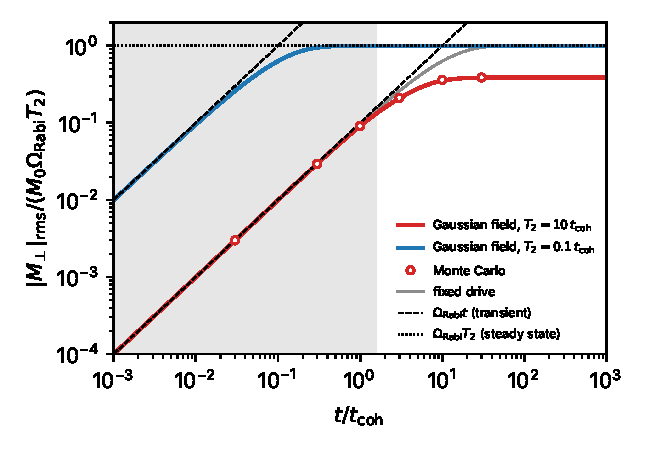
\includegraphics[width=0.92\linewidth]{figures/ch14/limit14_6a.pdf}
\captionof{figure}{Root-mean-square transverse magnetization of a nuclear-spin ensemble driven on resonance by an axion-like field, in units of $\Omega_{\mathrm{Rabi}}M_0T_2$, against the time over the coherence time $t_{\mathrm{coh}} = 1/m_\phi v_0^2$. Gray: the linear solution \cref{eq:14.6-mperp} for a drive of fixed amplitude, $1 - \ee^{-t/T_2}$, with its two literature limits, the transient $\Omega_{\mathrm{Rabi}}t$ (dashed) and the steady state $\Omega_{\mathrm{Rabi}}T_2$ (dotted). Colored: the same equation driven by the Gaussian field of the standard halo of \cref{sec:1.2} seen from the Earth, \cref{eq:14.6-ms}, with the Larmor frequency at the peak of the field line and $\Omega_{\mathrm{Rabi}}$ the value for the mean energy density; $T_2 = 10\,t_{\mathrm{coh}}$ (red) and $0.1\,t_{\mathrm{coh}}$ (blue). Circles: average over 1500 Monte Carlo realizations of the field for $T_2 = 10\,t_{\mathrm{coh}}$, each a sum of 2000 plane waves with random phases. Gray band: $t \le 1.6\,t_{\mathrm{coh}}$, where the field-averaged magnetization is within \SI{10}{\percent} of the fixed-drive formula for $T_2 = 10\,t_{\mathrm{coh}}$. For $T_2 = 0.1\,t_{\mathrm{coh}}$ the two agree within \SI{0.6}{\percent} at all times.}\label{fig:14-limit-mperp}
\par}
\smallskip
For $T_2 \gg t_{\mathrm{coh}}$ and $t \gtrsim t_{\mathrm{coh}}$ the magnetization stops growing linearly and saturates at $0.39$ of the fixed-drive value for $T_2 = 10\,t_{\mathrm{coh}}$; for longer $T_2$ the ratio falls as $(T_2/t_{\mathrm{coh}})^{-1/2}$.
\end{limitbox}

The linear solution assumes that the drive does not deplete $M_z$. At resonance and for $t \ll T_2$ the exact solution of \cref{eq:14.6-bloch} is $M_\perp = M_0\sin(\Omega_{\mathrm{Rabi}}t)$, below the linear one by the fraction $(\Omega_{\mathrm{Rabi}}t)^2/6$. In the steady state the $z$ component of \cref{eq:14.6-bloch} in the rotating frame gives $M_z = M_0/(1 + \Omega_{\mathrm{Rabi}}^2T_1T_2)$, and since $T_1$ is long, saturation sets in at drives with $\Omega_{\mathrm{Rabi}}T_2$ still small. Aybas and collaborators correct their limit by \SI{30}{\percent} for it at their detection threshold, $\Omega_{\mathrm{Rabi}} = \SI{0.23}{rad/s}$~\cite[Sect.~III]{aybas2021search}. The signal competes with noise from the spins themselves and from the magnetometer. The spin noise follows from the fluctuation--dissipation theorem \cref{eq:4.2-fdt} at the spin temperature $T_{\mathrm{s}}$ of a prepolarized sample, $p_{\mathrm{pol}} = \tanh(\omega_{\mathrm{Lar}}/2T_{\mathrm{s}})$. Since $\Imag R_{J_-J_-} \propto p_{\mathrm{pol}}$ while the symmetrized thermal factor is $\coth(\omega_{\mathrm{Lar}}/2T_{\mathrm{s}}) = 1/p_{\mathrm{pol}}$, the spin noise does not depend on the polarization~\cite[Eq.~(A1)]{budker2014proposal}, and prepolarization raises the signal only.

\subsection{The exponential-bin likelihood}\label{sec:14.6-stats}

A search records a readout for a time $t_{\mathrm{int}}$, the magnetometer signal of the precessing spins or the voltage of a resonator. It is demodulated at a carrier near $m_\phi$ into a complex signal $X(t)$ that holds both quadratures, and frequencies are measured from the carrier. The signal part is linear in the complex amplitude $\Phi$ of the field, $X_{\mathrm{sig}}(t) = \int\dd t'\,\mathcal{G}_{\mathrm{rd}}(t - t')\,\Phi(t')$ with a response kernel $\mathcal{G}_{\mathrm{rd}}$, and is thus Gaussian as well, with the power spectrum $\mathcal{S}_{\mathrm{sig}}(\omega) = |\mathcal{G}_{\mathrm{rd}}(\omega)|^2\mathcal{S}_\phi(\omega)$ up to the normalization of $\Phi$. For the spins, $|\mathcal{G}_{\mathrm{rd}}|^2$ is the Lorentzian of \cref{eq:14.6-mperp}; for a target much broader than the field line it is a constant, and $\mathcal{S}_{\mathrm{sig}}$ has the shape $F_\phi$. The noise, from the spins, the magnetometer or the amplifier, is Gaussian with the spectrum $\mathcal{S}_{\mathrm{n}}(\omega)$. The data are reduced to the periodogram at the frequencies $\omega_k = 2\pi k/t_{\mathrm{int}}$,
\begin{equation*}
  \mathsf{P}_k = \frac{1}{t_{\mathrm{int}}}\Bigl|\int_0^{t_{\mathrm{int}}}\dd t\,\ee^{\ii\omega_kt}X(t)\Bigr|^2 .
\end{equation*}
Its mean is the spectrum convolved with the Fejér kernel \cref{eq:14.6-fejer}, $\langle\mathsf{P}_k\rangle = \int\dd\omega\,\mathcal{K}_{t_{\mathrm{int}}}(\omega_k - \omega)[\mathcal{S}_{\mathrm{sig}}(\omega) + \mathcal{S}_{\mathrm{n}}(\omega)]$, which tends to $\mathcal{S}_{\mathrm{sig}}(\omega_k) + \mathcal{S}_{\mathrm{n}}(\omega_k)$ for a long record. The Fourier integral of a Gaussian process is a complex Gaussian variable, with independent real and imaginary parts of equal variance, and the sum of signal and noise is one such variable. Its squared modulus is exponentially distributed:
\begin{equation}
  p(\mathsf{P}_k) = \frac{1}{\bar{\mathsf{P}}_k}\,\ee^{-\mathsf{P}_k/\bar{\mathsf{P}}_k}, \qquad \bar{\mathsf{P}}_k = \mathsf{s}_k + \mathsf{b}_k ,
  \label{eq:14.6-expbin}
\end{equation}
with $\mathsf{s}_k$ and $\mathsf{b}_k$ the mean signal and noise powers of bin $k$. This is the distribution of Foster, Rodd and Safdi, with the mean $\mathsf{s}_k \propto F_\chi(v)/v \propto F_\phi(\omega_k)$ for a long record~\cite[Eq.~(24)]{foster2018revealing}. Signal and noise combine in the amplitudes, not in the powers; the sum of two exponential variables would not be exponential. For a record shorter than $t_{\mathrm{coh}}$ the whole line falls into one bin, and \cref{eq:14.6-expbin} states that the power in that bin, the square of the Rayleigh amplitude of the field, fluctuates by \SI{100}{\percent} from one realization to the next. For a longer record the line spreads over about $t_{\mathrm{int}}\Delta\omega_{\mathrm{eq}}/2\pi$ independent bins, each with its own exponential fluctuation. \Cref{fig:14-spectrum} shows single realizations, and \cref{lim:14.6b} the approach of the mean to its long-record form.

\begin{figure}[tbp]
  \centering
  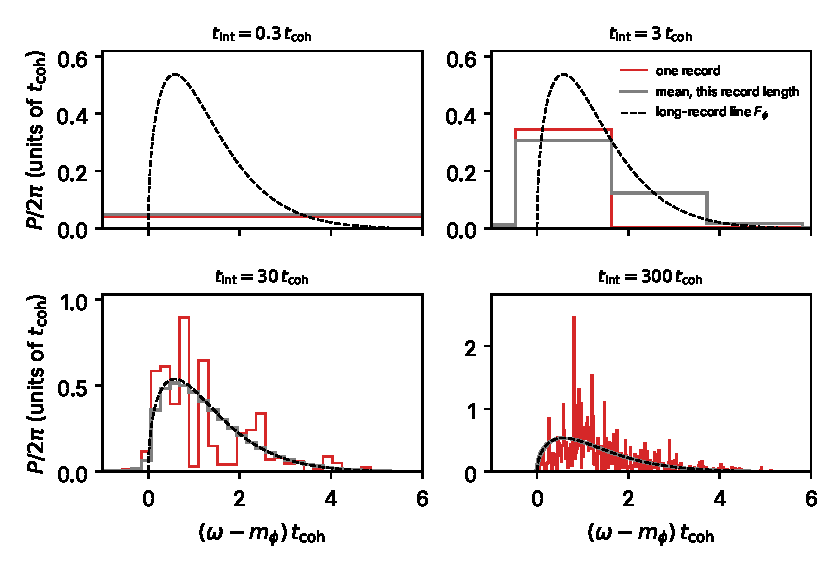
\includegraphics[width=0.92\linewidth]{figures/ch14/fig14_6.pdf}
  \caption{Periodogram of an axion-like field of unit mean power for records of $t_{\mathrm{int}} = 0.3$, 3, 30 and $300\,t_{\mathrm{coh}}$, against the energy above the rest energy in units of $1/t_{\mathrm{coh}} = m_\phi v_0^2$. Red: one Monte Carlo realization of the field, a sum of 3000 plane waves with random phases and with velocities from the standard halo of \cref{sec:1.2} seen from the Earth ($v_0 = \SI{238}{km/s}$, $v_{\mathrm{esc}} = \SI{544}{km/s}$, $v_E = \SI{250.5}{km/s}$). Bins of width $2\pi/t_{\mathrm{int}}$, one centered on the peak of the line. Gray: the mean periodogram for that record length, the line shape convolved with the Fejér kernel \cref{eq:14.6-fejer}. Dashed: the line shape $F_\phi$ of \cref{eq:14.6-Fphi}, the mean for a long record. Below $t_{\mathrm{coh}}$ one bin holds the whole line, with a height proportional to $t_{\mathrm{int}}$. Above it the bins resolve the line and scatter about it with the exponential distribution \cref{eq:14.6-expbin}.}
  \label{fig:14-spectrum}
\end{figure}

\begin{limitbox}[Gaussian-field signal and its power spectrum][lim:14.6b]
Exponential periodogram bins with mean $\mathsf{s}(\omega) \propto F_\phi(\omega)$, the line shape of \cref{eq:14.6-Fphi}, for a field built from Rayleigh-distributed amplitudes with random phases~\cite[Eqs.~(8), (10), (24)]{foster2018revealing}; for an absorber, the golden-rule mean of \cref{eq:8.2-abs} averaged over the line.
\par\smallskip
{\centering
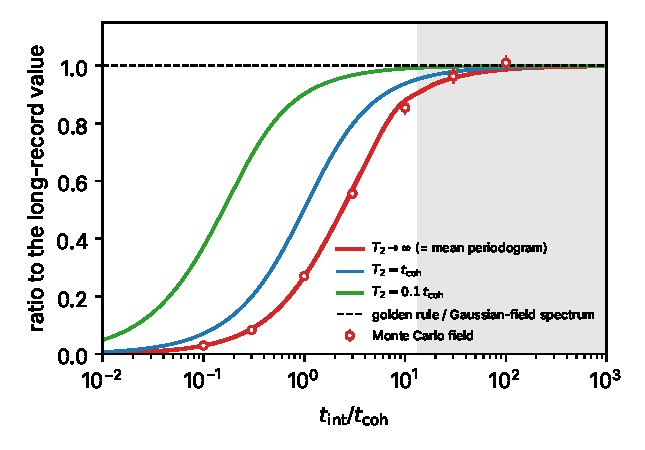
\includegraphics[width=0.92\linewidth]{figures/ch14/limit14_6b.pdf}
\captionof{figure}{Mean over the Gaussian field, for a record of length $t_{\mathrm{int}}$, divided by its long-record value, against $t_{\mathrm{int}}/t_{\mathrm{coh}}$. Red: the mean periodogram at the peak of the line, $\int\dd\omega\,F_\phi(\omega)\mathcal{K}_{t_{\mathrm{int}}}(\omega_{\mathrm{pk}} - \omega)/F_\phi(\omega_{\mathrm{pk}})$, which is also the energy absorbed by spins with $T_2 \to \infty$ at the peak frequency divided by the golden-rule value; circles: 1500 Monte Carlo realizations, with the scatter of their mean. Blue and green: energy absorbed by linearly driven spins with $T_2 = t_{\mathrm{coh}}$ and $0.1\,t_{\mathrm{coh}}$, divided by the golden-rule rate times $t_{\mathrm{int}}$. Standard halo of \cref{sec:1.2}. Gray band: the red curve within \SI{10}{\percent} of the long-record value, $t_{\mathrm{int}} \ge 13\,t_{\mathrm{coh}}$; for $T_2 = t_{\mathrm{coh}}$ and $0.1\,t_{\mathrm{coh}}$ the same accuracy needs $6.5\,t_{\mathrm{coh}}$ and $t_{\mathrm{coh}}$. The variance of the Monte Carlo bins equals the square of their mean within the sampling error, as the exponential law requires.}\label{fig:14-limit-spectrum}
\par}
\smallskip
Below $t_{\mathrm{coh}}$ and $T_2$ the mean grows as $t_{\mathrm{int}}^2$ rather than $t_{\mathrm{int}}$, with the ratio $t_{\mathrm{int}}/2\pi F_\phi(\omega_{\mathrm{pk}})$, and above them it approaches the golden rule as $1 - 1.25\,t_{\mathrm{coh}}/t_{\mathrm{int}}$, the leakage of the Fejér kernel.
\end{limitbox}

The bins of a stationary process are independent as long as the leakage of the Fejér kernel between neighbors is negligible. The likelihood of the periodogram is then the product of the distributions \cref{eq:14.6-expbin},
\begin{equation}
  -2\ln\mathsf{L} = 2\sum_k\Bigl[\ln\bar{\mathsf{P}}_k + \frac{\mathsf{P}_k}{\bar{\mathsf{P}}_k}\Bigr] ,
  \label{eq:14.6-like}
\end{equation}
the exponential-bin likelihood of Foster, Rodd and Safdi~\cite[Eq.~(29)]{foster2018revealing}, in which the signal enters through $\mathsf{s}_k$ and the coupling through its square, $\mathsf{s}_k \propto g^2$. Limits and discoveries follow from the likelihood ratio $\mathsf{t}$ of \cref{eq:C.14-ratio} and its thresholds \cref{eq:C.14-thresholds} (\cref{app:C.14}). How the sensitivity grows with $t_{\mathrm{int}}$ follows from the expected ratio for data without signal, $\mathsf{P}_k = \mathsf{b}_k$. Let $x_k = \mathsf{s}_k/\mathsf{b}_k$. Then $\mathsf{t} = 2\sum_k[\ln(1 + x_k) - x_k/(1 + x_k)]$, and for a weak signal, expanding to second order,
\begin{equation*}
  \mathsf{t} \simeq \sum_kx_k^2 = \frac{t_{\mathrm{int}}}{2\pi}\int\dd\omega\,\frac{\mathcal{S}_{\mathrm{sig}}(\omega)^2}{\mathcal{S}_{\mathrm{n}}(\omega)^2} ,
\end{equation*}
where the sum over bins of width $2\pi/t_{\mathrm{int}}$ became an integral. Let $\sigma_{\mathrm{sig}}^2$ be the mean square of the signal, proportional to $g^2$, and take white noise. For a record shorter than $t_{\mathrm{coh}}$ one bin holds the signal, $\mathsf{s} = \sigma_{\mathrm{sig}}^2t_{\mathrm{int}}$ and $\mathsf{b} = \mathcal{S}_{\mathrm{n}}$, so a fixed threshold on $\mathsf{t}$ means a fixed $x$, and
\begin{equation}
  \sigma_{\mathrm{sig}} \propto \mathcal{S}_{\mathrm{n}}^{1/2}\,t_{\mathrm{int}}^{-1/2}\quad(t_{\mathrm{int}} \ll t_{\mathrm{coh}}), \qquad
  \sigma_{\mathrm{sig}} \propto \mathcal{S}_{\mathrm{n}}^{1/2}\,(t_{\mathrm{int}}t_{\mathrm{coh}})^{-1/4}\quad(t_{\mathrm{int}} \gg t_{\mathrm{coh}}) .
  \label{eq:14.6-scaling}
\end{equation}
For a long record the integral gives $\mathsf{t} = 2\pi t_{\mathrm{int}}\sigma_{\mathrm{sig}}^4/(\Delta\omega_{\mathrm{eq}}\mathcal{S}_{\mathrm{n}}^2)$ with $\Delta\omega_{\mathrm{eq}} = 2.67/t_{\mathrm{coh}}$, which is the second law. Inside one coherence time the signal adds in amplitude and the noise in power, the familiar $t^{-1/2}$ of a coherent sinusoid. Beyond it the signal power stops growing in each bin, and only the number of bins over which the line is averaged grows, as $t_{\mathrm{int}}$, which halves the exponent. These are the scalings of Budker and collaborators~\cite[Eqs.~(A7), (A8)]{budker2014proposal}; the long-record form, with the coefficient of the weak-signal ratio, is the expected limit of Foster, Rodd and Safdi~\cite[Eqs.~(54), (63), (69)]{foster2018revealing}. For the spins, $\sigma_{\mathrm{sig}} = |M_\perp|$ is proportional to $g$, and the coupling at the threshold scales as $\sigma_{\mathrm{sig}}$.

The amplitude of the field within one coherence time is a random draw, and an analysis that ignores this sets too strong a limit. A search shorter than $t_{\mathrm{coh}}$ that takes the amplitude fixed at its mean value $\sqrt{2\rho_\chi}/m_\phi$ excludes every coupling whose signal would have exceeded the noise in that one realization; however, the field may have been weak during the record, with probability $1 - \ee^{-a}$ for an intensity below $a$ times its mean. Centers and collaborators found that limits with a fixed amplitude are too strong by a factor of 3 in a Bayesian treatment and 2.7 in a frequentist one, up to 10 with other priors, and 8.4 for gradient couplings~\cite[Eq.~(7)]{centers2021stochastic}. The exponential-bin likelihood already contains the random amplitude, so the correction is made once: with the likelihood \cref{eq:14.6-like}, or with a fixed-amplitude likelihood followed by the correction factor, never both.

An exact Neyman construction gives the size of the correction. Replace the line of the standard halo, convolved with the Fejér kernel, by $N_{\mathrm{eff}}$ equal bins, with $N_{\mathrm{eff}} = 1/\sum_kp_k^2$ the participation number of the bin fractions $p_k$ ($N_{\mathrm{eff}} \to 1$ below $t_{\mathrm{coh}}$ and $t_{\mathrm{int}}\Delta\omega_{\mathrm{eq}}/2\pi$ above). The bins have the width $2\pi/t_{\mathrm{int}}$, with one bin centered on the peak of the line. The statistic is the summed periodogram $\mathsf{Q}$ of those bins, with noise $\mathsf{b}$ per bin and total signal $\mathsf{s} = \sigma_{\mathrm{sig}}^2t_{\mathrm{int}}$ at every record length. With the Rayleigh amplitude of \cref{eq:14.6-expbin}, $\mathsf{Q}$ follows a Gamma distribution of shape $N_{\mathrm{eff}}$ and scale $\mathsf{b} + \mathsf{s}/N_{\mathrm{eff}}$; with a fixed amplitude and random phase, $2\mathsf{Q}/\mathsf{b}$ follows a noncentral $\chi^2$ distribution with $2N_{\mathrm{eff}}$ degrees of freedom and noncentrality $2\mathsf{s}/\mathsf{b}$. The \SI{95}{\percent} upper limit $\mathsf{s}_{\mathrm{up}}$ solves $P(\mathsf{Q} \le \mathsf{Q}_{\mathrm{obs}}\,|\,\mathsf{s}_{\mathrm{up}}) = 0.05$, with $\mathsf{Q}_{\mathrm{obs}}$ the median of the Gamma distribution of shape $N_{\mathrm{eff}}$ and scale $\mathsf{b}$ for data without signal. For the median of data without signal and one bin, $\mathsf{s}_{\mathrm{up}}/\mathsf{b} = 12.5$ with the Rayleigh amplitude and 3.17 with a fixed one, so that the fixed amplitude sets a coupling limit lower by $(12.5/3.17)^{1/2} = 1.99$. For data at the detection threshold, $\mathsf{Q}_{\mathrm{obs}} = \mathsf{b}\ln20$, the same construction gives 57.4 and 7.72 and a factor 2.73. \Cref{lim:14.6c} shows both treatments against the record length.
\begin{limitbox}[Sensitivity scalings of the exponential-bin likelihood][lim:14.6c]
Threshold amplitude $\propto\mathcal{S}_{\mathrm{n}}^{1/2}t_{\mathrm{int}}^{-1/2}$ for $t_{\mathrm{int}} < t_{\mathrm{coh}}$ and $\propto\mathcal{S}_{\mathrm{n}}^{1/2}(t_{\mathrm{int}}t_{\mathrm{coh}})^{-1/4}$ for $t_{\mathrm{int}} > t_{\mathrm{coh}}$~\cites[Eqs.~(A7), (A8)]{budker2014proposal}[Eqs.~(54), (63), (69)]{foster2018revealing}.
\par\smallskip
{\centering
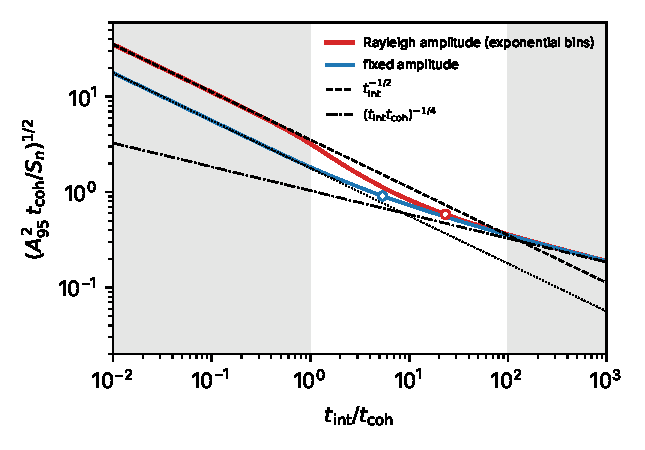
\includegraphics[width=0.92\linewidth]{figures/ch14/limit14_6c.pdf}
\captionof{figure}{Signal amplitude at the median expected \SI{95}{\percent} upper limit, $(\sigma_{\mathrm{sig}}^2t_{\mathrm{coh}}/\mathcal{S}_{\mathrm{n}})^{1/2}$, proportional to the coupling, against the record length over the coherence time, for white noise of spectrum $\mathcal{S}_{\mathrm{n}}$. Red: the signal as a Gaussian variable with a Rayleigh amplitude, the exponential-bin likelihood \cref{eq:14.6-like}. Blue: the signal power in each bin taken as fixed, with a random phase. Both curves follow from the Neyman construction of the text, with $N_{\mathrm{eff}}$ equal bins for the line of the standard halo of \cref{sec:1.2}. Dashed: $t_{\mathrm{int}}^{-1/2}$ for the Rayleigh amplitude (dotted: fixed amplitude); dash-dotted: $(t_{\mathrm{int}}t_{\mathrm{coh}})^{-1/4}$, common to both. Circles: the crossover, where the local slope is $-3/8$, at $23\,t_{\mathrm{coh}}$ (Rayleigh) and $5.4\,t_{\mathrm{coh}}$ (fixed). Gray: the Rayleigh curve within \SI{10}{\percent} of the $t_{\mathrm{int}}^{-1/2}$ law ($t_{\mathrm{int}} \le t_{\mathrm{coh}}$) or of the $(t_{\mathrm{int}}t_{\mathrm{coh}})^{-1/4}$ law ($t_{\mathrm{int}} \ge 100\,t_{\mathrm{coh}}$).}\label{fig:14-limit-scaling}
\par}
\smallskip
Neither power law holds between $t_{\mathrm{coh}}$ and $100\,t_{\mathrm{coh}}$, where the Rayleigh curve falls as steeply as $t_{\mathrm{int}}^{-0.67}$, faster than either law, because the record begins to average over independent amplitudes.
\end{limitbox}

The fixed amplitude sets a limit lower by 1.99 for records below $t_{\mathrm{coh}}$, by 1.76 at $t_{\mathrm{coh}}$ and by \SI{1.5}{\percent} at $100\,t_{\mathrm{coh}}$. The two power laws, extended, meet at $136\,t_{\mathrm{coh}}$ for the Rayleigh amplitude and at $8.7\,t_{\mathrm{coh}}$ for the fixed one, so the crossover lies between a few and about a hundred coherence times and its coefficient is not universal.

\begin{workedexample}{The scaling crossover for a \SI{1}{neV} axion-like field}\label{we:14-crossover}
An axion-like field of $m_\phi = \SI{1}{neV}$ oscillates at $m_\phi/2\pi = \SI{241.8}{kHz}$. By \cref{eq:14.6-tcoh}, $t_{\mathrm{coh}} = \SI{1.044}{s}$, and its line has the equivalent width $\Delta\omega_{\mathrm{eq}}/2\pi = 2.67/(2\pi t_{\mathrm{coh}}) = \SI{0.41}{Hz}$, $1.7\times10^{-6}$ of the frequency.

A $^{207}$Pb sample resonates at this frequency in $B_0 = 241.8\,\mathrm{kHz}/(9.034\,\mathrm{MHz\,T^{-1}}) = \SI{26.8}{mT}$. Its $T_2 = \SI{16.7}{ms}$ is $0.016\,t_{\mathrm{coh}}$, so the spin line, of half width $1/T_2 = \SI{60}{s^{-1}}$, is 63 times wider than the field line, $m_\phi v_0^2 = \SI{0.96}{s^{-1}}$. The spins are in the case $T_2 \ll t_{\mathrm{coh}}$ of \cref{lim:14.6a}: the magnetization reaches the steady state of \cref{eq:14.6-mperp} after a few $T_2$, about \SI{0.05}{s}, and its amplitude then follows the Rayleigh amplitude of the field, which changes on the scale of a second.

The sensitivity depends on how long a record at one frequency can be. With the construction of \cref{lim:14.6c}, the threshold coupling falls by a factor 3.46 from $t_{\mathrm{int}} = \SI{0.1}{s}$ to \SI{1}{s}, more than the $\sqrt{10} = 3.16$ of the coherent law, since the record starts to sample a second amplitude. The local slope reaches $-3/8$ at $23\,t_{\mathrm{coh}} = \SI{24}{s}$. A record of one hour spans 3447 coherence times and a day 82\,730. Going from an hour to a day improves the limit by 2.24, close to $24^{1/4} = 2.21$ and far from the $24^{1/2} = 4.9$ that a coherent signal would give. At \SI{0.1}{s} the fixed-amplitude analysis would claim a limit 1.99 times lower; at one hour the two agree to better than \SI{0.1}{\percent}.
\end{workedexample}

A search that scans the field over a decade of frequency in a fixed total time spends less time at each frequency as the line narrows toward low masses. The crossover then decides whether to dwell longer at one frequency or to scan more. At $m_\phi = \SI{1}{\micro eV}$, $t_{\mathrm{coh}} = \SI{1.04}{ms}$, and every practical record lies deep in the $(t_{\mathrm{int}}t_{\mathrm{coh}})^{-1/4}$ regime; at \SI{1}{peV}, $t_{\mathrm{coh}} = \SI{17}{min}$, and the random amplitude must be in the likelihood.

\section{Chiral and nonreciprocal targets}\label{sec:14.5}

Density-functional perturbation theory gives $\alpha$-quartz the gyration $g_{33} = \SI{0.125}{bohr}$ along its optic axis, and with it a rotation of the plane of polarization by \SI{21.6}{\degree} per millimeter for light of \SI{2.105}{eV}~\cite[Table~I, Eq.~(4)]{zabalo2023natural}; the mirror-image crystal turns the plane the other way. The rotation is a response odd in the momentum of the light, and at a photon momentum of \SI{2.1}{eV} it is small, $q\,g_{33} = 7\times10^{-5}$. Dark matter that deposits the same energy brings at least $1/v_{\mathrm{max}} = 377$ times more momentum, so a response odd in $\vect{q}$ may matter more for dark matter than for light. \Cref{sec:11.7} showed that the density response stays even in $\vect{q}$ unless inversion and time reversal are both broken; in a crystal, magnetic order breaks time reversal. Here we find which other responses become odd when only one of the two symmetries is broken, in which crystals, and which couplings of the dark matter see them. Three detectors are built on broken symmetry: phonons that carry angular momentum, molecular magnets held in a metastable state, and multiferroics, in which electric and magnetic order coexist.

\subsection{Reciprocity of the response matrix}\label{sec:14.5-recip}

Time reversal relates the response at $\vect{q}$ to that at $-\vect{q}$ for every pair of rows. Each row of \cref{eq:8.1-rows} goes over into itself at $-\vect{q}$ under the antiunitary time-reversal operator $\mathsf{T}$, up to a sign $\sigma^{\mathsf{T}}_a$: $\mathsf{T}O_a(\vect{q})\mathsf{T}^{-1} = \sigma^{\mathsf{T}}_aO_a(-\vect{q})$, since $\mathsf{T}$ conjugates $\ee^{\ii\vect{q}\cdot\vect{r}}$ and reverses momenta and spins. The density and the kinetic-energy density have $\sigma^{\mathsf{T}} = +1$, the current and the spin density $-1$, and the spin current $+1$, as the product of two reversed vectors. For an antiunitary operator, $\langle f|A|i\rangle^* = \langle\mathsf{T}f|\mathsf{T}A\mathsf{T}^{-1}|\mathsf{T}i\rangle$. We apply this identity to both matrix elements in \cref{eq:4.2-Sab}; the time-reversed states carry the same energies and thermal weights, so $S_{ab}(\vect{q},\omega)^* = \sigma^{\mathsf{T}}_a\sigma^{\mathsf{T}}_bS_{ab}(-\vect{q},\omega)$. With $S_{ab}^* = S_{ba}$,
\begin{equation}
  \begin{aligned}
  S_{ab}(\vect{q},\omega) &= \sigma^{\mathsf{T}}_a\sigma^{\mathsf{T}}_b\,S_{ba}(-\vect{q},\omega) &&(\text{time reversal}), \\
  S_{ab}(\vect{q},\omega) &= \sigma^{\mathsf{P}}_a\sigma^{\mathsf{P}}_b\,S_{ab}(-\vect{q},\omega) &&(\text{inversion}) .
  \end{aligned}
  \label{eq:14.5-recip}
\end{equation}
The second relation follows in the same way from the unitary inversion $\mathsf{P}$, with $\sigma^{\mathsf{P}} = +1$ for the density, the kinetic-energy density and the spin density and $-1$ for the current and the spin current. For the density block alone both relations give $S(\vect{q}) = S(-\vect{q})$ (\cref{app:A.4}).

The current block is the first that differs. Hermiticity splits it into a real symmetric part and $\ii$ times a real antisymmetric part, and an antisymmetric $3\times3$ matrix is a vector:
\begin{equation}
  S_{j^\alpha j^\beta}(\vect{q},\omega) = S^{\mathrm{R}}_{\alpha\beta}(\vect{q},\omega) + \ii\,\epsilon_{\alpha\beta\gamma}\,\mathcal{G}^\gamma_{\mathrm{OA}}(\vect{q},\omega) .
  \label{eq:14.5-GOA}
\end{equation}
With $\sigma^{\mathsf{T}}_j = -1$ twice, time reversal gives $S_{j^\alpha j^\beta}(\vect{q}) = S_{j^\alpha j^\beta}(-\vect{q})^*$: the symmetric part is even in $\vect{q}$ and $\boldsymbol{\mathcal{G}}_{\mathrm{OA}}$ is odd. Since inversion makes both parts even, $\boldsymbol{\mathcal{G}}_{\mathrm{OA}}$ needs a crystal without inversion and survives time reversal, while an odd symmetric part needs both symmetries broken. A crystal without inversion, mirror planes or rotation--reflections is chiral, and exists in two forms related by a mirror, its enantiomers; $\boldsymbol{\mathcal{G}}_{\mathrm{OA}}$ changes sign between them. Physically, $\boldsymbol{\mathcal{G}}_{\mathrm{OA}}$ measures whether the electrons circulate one way more easily than the other along $\vect{q}$, an asymmetry that only a crystal without inversion allows. For rows of opposite time-reversal sign, such as the spin density and the spin current, \cref{eq:14.5-recip} makes the symmetric part of the block odd in $\vect{q}$, so its value at $\vect{q} = 0$, which a static field would probe, needs inversion broken as well. \Cref{tab:14-odd} collects the cases that this section uses.

\begin{table}[tbp]
  \caption{Parts of the response odd in $\vect{q}$, or odd under inversion of the crystal, and the symmetries they need, from \cref{eq:14.5-recip}. ``Gyrotropic'' point groups are those with $N_{\mathrm{gyr}} > 0$ in \cref{eq:C.17-gyration}.}
  \label{tab:14-odd}
  \centering\small
  \begin{tabular}{@{}>{\raggedright\arraybackslash}p{0.30\linewidth}>{\raggedright\arraybackslash}p{0.27\linewidth}>{\raggedright\arraybackslash}p{0.33\linewidth}@{}}
    \toprule
    Quantity & Needs & Treated in \\
    \midrule
    Density $S(\vect{q},\omega) - S(-\vect{q},\omega)$ & inversion and time reversal broken & \cref{sec:11.7} \\
    Antisymmetric current part $\boldsymbol{\mathcal{G}}_{\mathrm{OA}}$ & inversion broken, gyrotropic group & \cref{sec:14.5-oa}, \cref{we:14-quartz} \\
    Symmetric current part, odd in $\vect{q}$ & inversion and time reversal broken & \cref{sec:14.5-recip} \\
    Phonon angular momentum $\vect{L}^{\mathrm{ph}}$ & inversion or time reversal broken & \cref{sec:14.5-phonons} \\
    Static spin--spin-current block $R_{s^z\mathcal{J}}(0,\omega \to 0)$ & inversion and time reversal broken & \cref{sec:14.5-mf} \\
    \bottomrule
  \end{tabular}
\end{table}

\subsection{Finite-momentum optical activity}\label{sec:14.5-oa}

The vector $\boldsymbol{\mathcal{G}}_{\mathrm{OA}}$ is the finite-momentum generalization of natural optical activity. To see the connection, write the antisymmetric part of the proper current response as $\ii\epsilon_{\alpha\beta\gamma}\mathcal{G}^\gamma_{\mathrm{R}}$, with $\boldsymbol{\mathcal{G}}_{\mathrm{R}}$ complex. The fluctuation--dissipation theorem \cref{eq:4.2-fdt}, $(1 - \ee^{-\beta\omega})S_{ab} = \ii(R_{ab} - R_{ba}^*)$, gives $\boldsymbol{\mathcal{G}}_{\mathrm{OA}} = -2\Imag\boldsymbol{\mathcal{G}}_{\mathrm{R}}/(1 - \ee^{-\beta\omega})$, and the dielectric tensor of \cref{sec:4.4}, $\varepsilon^{\alpha\beta} = \delta^{\alpha\beta} - (e^2/\omega^2)[(\nd_e/m_e)\delta^{\alpha\beta} + \tilde R^{\alpha\beta}_{jj}]$, acquires the antisymmetric term $-\ii(e^2/\omega^2)\epsilon_{\alpha\beta\gamma}\mathcal{G}^\gamma_{\mathrm{R}}$. Optical activity is defined by the term linear in $\vect{q}$ of that tensor, $\varepsilon^{\alpha\beta}(\vect{q},\omega) = \varepsilon^{\alpha\beta}(\omega) + \ii\epsilon_{\alpha\beta m}g_{ml}(\omega)q_l + O(q^2)$, with the gyration tensor $g_{ml}$ of \cref{app:C.17} in the normalization of the dielectric tensor~\cite[Eqs.~(2)--(4)]{zabalo2023natural}. Comparing the two antisymmetric terms,
\begin{equation}
  \mathcal{G}^\gamma_{\mathrm{OA}}(\vect{q},\omega) = \frac{2\omega^2}{e^2}\,\frac{\Imag g_{\gamma l}(\omega)\,q_l}{1 - \ee^{-\beta\omega}} + O(q^3) ,
  \label{eq:14.5-gyr}
\end{equation}
with no term of order $q^2$, since $\boldsymbol{\mathcal{G}}_{\mathrm{OA}}$ is odd. Only the absorptive part of the gyration enters the structure factor. The reactive part of the gyration, $\Real g$, rotates the polarization, and the absorptive and reactive parts are related by the Kramers--Kronig relations \cref{eq:4.3-KK}, which hold for $g(\omega)$ because $g(\omega)$ is a coefficient of a causal response.

The observable is circular dichroism, the difference between the absorption of the two helicities. A transverse field of polarization $\hat{\vect{e}}_\pm = (\hat{\vect{e}}_1 \pm \ii\hat{\vect{e}}_2)/\sqrt2$, with $\hat{\vect{e}}_1\times\hat{\vect{e}}_2 = \hat{\vect{q}}$, couples to the row $\hat{\vect{e}}_\pm\cdot\vect{j}_e$, and \cref{eq:8.2-abs} needs $\sum_{\alpha\beta}\hat e^*_{\pm\alpha}\hat e_{\pm\beta}S_{j^\alpha j^\beta}$. The symmetric part yields the transverse response $S_{\mathrm{T}}$, and the antisymmetric part gives $\ii(\hat{\vect{e}}^*_\pm\times\hat{\vect{e}}_\pm)\cdot\boldsymbol{\mathcal{G}}_{\mathrm{OA}}$ with $\hat{\vect{e}}^*_\pm\times\hat{\vect{e}}_\pm = \pm\ii\hat{\vect{q}}$:
\begin{equation}
  S_\pm(\vect{q},\omega) = S_{\mathrm{T}}(\vect{q},\omega) \mp \hat{\vect{q}}\cdot\boldsymbol{\mathcal{G}}_{\mathrm{OA}}(\vect{q},\omega), \qquad
  \frac{S_- - S_+}{S_- + S_+} = \frac{\hat{\vect{q}}\cdot\boldsymbol{\mathcal{G}}_{\mathrm{OA}}}{S_{\mathrm{T}}} = \frac{q\,\Imag g_{\hat q\hat q}}{\varepsilon_2^{\mathrm{T}}} ,
  \label{eq:14.5-helicity}
\end{equation}
with $g_{\hat q\hat q} = \hat{\vect{q}}\cdot g\cdot\hat{\vect{q}}$; the last form uses \cref{eq:14.5-gyr} and $\varepsilon_2^{\mathrm{T}} = (e^2/2\omega^2)(1 - \ee^{-\beta\omega})S_{\mathrm{T}}$ at the order kept. Reversing $\vect{q}$ at fixed helicity exchanges $\hat{\vect{e}}_1$ and $\hat{\vect{e}}_2$ up to sign and flips $\boldsymbol{\mathcal{G}}_{\mathrm{OA}}$, so the dissymmetry depends on the helicity, not on the direction of travel: natural optical activity is reciprocal. For light, $q = n_r\omega$ with $n_r$ the refractive index, and the helicity components of $\varepsilon$ are $\varepsilon^{\mathrm{T}} \mp g_{\hat q\hat q}q$. Then $n_\pm = n_r \mp g_{\hat q\hat q}\omega/2$, and per unit length the plane of linear polarization turns by
\begin{equation}
  \rho(\omega) = \frac{\omega}{2}\Real(n_- - n_+) = \frac{\omega^2}{2}\Real g_{\hat q\hat q}(\omega) ,
  \label{eq:14.5-rot}
\end{equation}
the rotatory power of Zabalo and Stengel~\cite[Eq.~(4)]{zabalo2023natural}, while the absorption coefficients of the two helicities differ by $2\omega^2\Imag g_{\hat q\hat q}$.

\Cref{fig:14-cd} sketches what changes for dark matter. At optical momenta the dissymmetry is of order $q|g| \sim 10^{-4}$. Dark matter at energy $\omega$ brings $q \ge \omega/v_{\mathrm{max}}$, and at $q = \SI{1}{keV}$ the quartz value of $g_{33}$ gives $q\,g_{33} = 0.034$. The value 0.034 sets a scale only. \Cref{eq:14.5-gyr} holds for $q$ small against the inverse lattice spacing, while dark-matter momenta of keV reach the zone boundary, and above the band gap of quartz the absorptive $\Imag g$, not the static $g_{33}$, is the relevant input. The full $\boldsymbol{\mathcal{G}}_{\mathrm{OA}}(\vect{q},\omega)$ at keV momenta is not known for any crystal.

\begin{figure}[tbp]
  \centering
  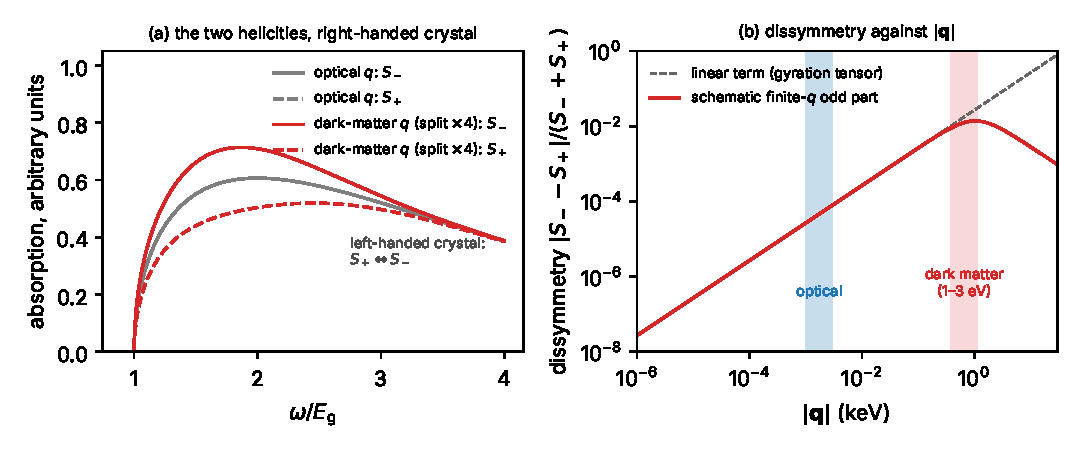
\includegraphics[width=0.95\linewidth]{figures/ch14/fig14_5.pdf}
  \caption{Circular dichroism of a chiral crystal such as tellurium. Schematic: all curves are model curves, not computed for tellurium. (a) Absorption of the two helicities, $S_\pm = S_{\mathrm{T}} \mp \hat{\vect{q}}\cdot\boldsymbol{\mathcal{G}}_{\mathrm{OA}}$ (\cref{eq:14.5-helicity}), for a model band edge at $E_{\mathrm{g}}$ in the right-handed form, at an optical momentum (gray, split invisible) and at a dark-matter momentum (red, split exaggerated four times). The left-handed form exchanges $S_+$ and $S_-$. (b) The dissymmetry against $|\vect{q}|$: the linear term $q|g|$ with $|g| = \SI{0.1}{bohr}$, the order of the computed gyration of trigonal crystals~\cite[Table~I]{zabalo2023natural} (dashed), and a schematic turnover at the inverse of a \SI{6}{\angstrom} helix pitch (red). Blue band: photons of 1 to \SI{3}{eV}; red band: the smallest dark-matter momenta at the same energies, $\omega/v_{\mathrm{max}}$. The odd part beyond the linear term is not known.}
  \label{fig:14-cd}
\end{figure}

Dark matter sees $\boldsymbol{\mathcal{G}}_{\mathrm{OA}}$ only through a coupling tensor with an antisymmetric current block. In \cref{tab:8-operators} the current row of $\mathcal{O}_5$ has the potential $\tilde V_{j^\delta} = -(\ii/m_e)c_5\epsilon_{\mu\gamma\delta}S^\mu_\chi q^\gamma$, and that of $\mathcal{O}_8$ has $\tilde V_{j^\delta} = -c_8S^\delta_\chi$. Each alone leads to a real symmetric $\mathfrak{D}_{jj}$: $\frac14|c_8|^2\delta_{\alpha\beta}$ for $\mathcal{O}_8$ and $(|c_5|^2/4m_e^2)(q^2\delta_{\alpha\beta} - q_\alpha q_\beta)$ for $\mathcal{O}_5$. Their interference, with $\Tr_\chi(S^\mu_\chi S^\nu_\chi)/2 = \delta_{\mu\nu}/4$ in \cref{eq:8.1-D}, gives
\begin{equation*}
  \mathfrak{D}_{j^\alpha j^\beta} \supset -\frac{\ii}{2m_e}\,\Real(c_5^*c_8)\,\epsilon_{\alpha\beta\gamma}q^\gamma ,
\end{equation*}
purely imaginary and antisymmetric, and its contraction with \cref{eq:14.5-GOA} is $(1/m_e)\Real(c_5^*c_8)\,\vect{q}\cdot\boldsymbol{\mathcal{G}}_{\mathrm{OA}}$. Since $\boldsymbol{\mathcal{G}}_{\mathrm{OA}}$ changes sign between enantiomers, the difference of their rates isolates this term. The density rows of $\mathcal{O}_5$ and $\mathcal{O}_8$ meet the current rows through the block $S_{nj}$. Inversion maps one enantiomer onto the other and, by \cref{eq:14.5-recip} with $\sigma^{\mathsf{P}}_n\sigma^{\mathsf{P}}_j = -1$, gives $S^{\mathrm{L}}_{nj}(\vect{q}) = -S^{\mathrm{R}}_{nj}(-\vect{q})$, so the enantiomer-odd part $S^{\mathrm{R}}_{nj}(\vect{q}) - S^{\mathrm{L}}_{nj}(\vect{q})$ is a vector even in $\vect{q}$. Averaged over crystal orientations at fixed $\vect{q}$, the enantiomer-odd part must point along $\hat{\vect{q}}$. A vector even in $\vect{q}$ cannot point along $\hat{\vect{q}}$, so the average vanishes; the enantiomer-odd part also enters contracted with $\vect{q}\times\bar{\vect{v}}_\chi$, which is orthogonal to $\hat{\vect{q}}$. Inserting the interference term in \cref{eq:8.2-spectrum} and averaging over orientations with the kernel $\eta(\vmin)/2q$ of \cref{eq:A.8-eta} gives
\begin{keyresult}[Enantiomer difference of the rate]
\begin{equation}
  \frac{\dd\mathcal{R}^{\mathrm{R}}}{\dd\omega} - \frac{\dd\mathcal{R}^{\mathrm{L}}}{\dd\omega}
  = \frac{\rho_\chi}{\mchi\,\rho_T}\int\frac{q\,\dd q}{2\pi^2}\,\eta(\vmin)\,\frac{q}{m_e}\,\Real\bigl[c_5^*(q)\,c_8(q)\bigr]\,\bar{\mathcal{G}}_{\mathrm{OA}}(q,\omega) ,
  \label{eq:14.5-enant}
\end{equation}
with $\bar{\mathcal{G}}_{\mathrm{OA}}(q,\omega)$ the average of $\hat{\vect{q}}\cdot\boldsymbol{\mathcal{G}}_{\mathrm{OA}}$ over the directions of $\vect{q}$ in the right-handed form.
\end{keyresult}
\noindent Operator $\mathcal{O}_8 = \vect{S}_\chi\cdot\vect{v}^\perp$ is odd under inversion and $\mathcal{O}_5$ is even. Only dark matter whose couplings violate parity therefore has different rates in the two enantiomers, for example a particle with both a magnetic dipole moment, which produces $\mathcal{O}_5$, and an anapole moment, which produces $\mathcal{O}_8$ (\cref{sec:8.1}). The couplings supply one parity-odd factor, and the crystal supplies the other, $\boldsymbol{\mathcal{G}}_{\mathrm{OA}}$. Because $\vect{q}\cdot\boldsymbol{\mathcal{G}}_{\mathrm{OA}}$ is even in $\vect{q}$, the enantiomer difference is not a wind asymmetry: at fixed orientation it contains the multipoles $\ell = 0$ and $\ell = 2$ of \cref{eq:11.7-rate} and modulates with the even halo multipoles. Relative to the transverse-current part of the rate of $\mathcal{O}_8$ alone, $\frac12|c_8|^2S_{\mathrm{T}}$, the interference term is the dissymmetry of \cref{eq:14.5-helicity} at dark-matter momenta times $2|c_5|q/(m_e|c_8|)$.

\begin{workedexample}{Point-group test for odd responses in $\alpha$-quartz}\label{we:14-quartz}
$\alpha$-Quartz, like tellurium, has the point group $32$ ($D_3$): the identity, two rotations by $\pm2\pi/3$ about the optic axis $\hat{\vect{z}}$, and three rotations by $\pi$ about twofold axes in the basal plane. All six are proper, $\det\mathsf{R} = 1$, and the class values of $1 + 2\cos\theta_{\mathsf{R}}$ are $3$, $0$ and $-1$ (\cref{app:C.17}).

\emph{Scalar responses.} An odd part of a scalar such as $S(\vect{q},\omega)$ starts with the harmonics $\ell = 1$, which transform as a polar vector. By \cref{eq:C.17-ninv,eq:C.17-polar} their invariants number $(3 + 2\cdot0 + 3\cdot(-1))/6 = 0$. The harmonics $\ell = 3$, with characters $\sin(\frac72\theta)/\sin(\frac12\theta) = 7$, $1$, $-1$, have $(7 + 2 - 3)/6 = 1$ invariant. Quartz keeps time reversal, however, and by \cref{eq:14.5-recip} its density response is even anyway; a magnetic crystal with the same point group could have a scalar odd part starting at $\ell = 3$, never at $\ell = 1$, because the group is not polar.

\emph{The current response.} The gyration tensor transforms with $(\det\mathsf{R})(1 + 2\cos\theta_{\mathsf{R}})^2 = 9$, $0$, $1$ on the three classes, and \cref{eq:C.17-gyration} gives $N_{\mathrm{gyr}} = (9 + 0 + 3)/6 = 2$. Projecting all nine components with $|\mathcal{P}|^{-1}\sum_{\mathsf{R}}(\det\mathsf{R})\,\mathsf{R}\otimes\mathsf{R}$ leaves the two diagonal tensors $\operatorname{diag}(1,1,0)$ and $\operatorname{diag}(0,0,1)$, so $g = \operatorname{diag}(g_{11}, g_{11}, g_{33})$. The density-functional values are $g_{11} = \SI{-0.071}{bohr}$ and $g_{33} = \SI{0.125}{bohr}$~\cite[Table~I]{zabalo2023natural}.

\emph{Consequences.} Along the optic axis, $g_{\hat q\hat q} = g_{33}$ and \cref{eq:14.5-rot} gives $\rho = \SI{21.6}{\degree.mm^{-1}}$ at \SI{2.105}{eV}. Averaged over directions, $g_{\hat q\hat q}$ becomes $(2g_{11} + g_{33})/3 = \SI{-0.0057}{bohr}$, only $-0.045$ of $g_{33}$, because $g_{11}$ and $g_{33}$ have opposite signs. If the same cancellation held for $\Imag g$ above the gap, the orientation-averaged enantiomer difference \cref{eq:14.5-enant} of quartz would be twenty times smaller than the difference for $\vect{q}$ along the optic axis. A crystal held with its axis along the wind would gain the factor of twenty back through the multipole $\ell = 2$. GaAs, with $N_{\mathrm{gyr}} = 0$ (\cref{we:C-gyration}), has no $\boldsymbol{\mathcal{G}}_{\mathrm{OA}}$ at linear order although it lacks inversion, and no enantiomers.
\end{workedexample}

\subsection{Chiral phonons}\label{sec:14.5-phonons}

In GaAs, which lacks inversion, the atoms in a phonon of a general wavevector move on ellipses, and a phonon of the lowest band carries on average $0.12$ units of angular momentum. In the normalization of \cref{eq:5.3-u}, the angular momentum of mode $\vect{Q}\nu$ in units of $\hbar$ is
\begin{equation}
  \vect{L}^{\mathrm{ph}}_{\vect{Q}\nu} = \sum_\kappa\vect{L}^{\mathrm{ph}}_{\kappa,\vect{Q}\nu}, \qquad
  \vect{L}^{\mathrm{ph}}_{\kappa,\vect{Q}\nu} = -\ii\,\vect{e}_{\kappa\nu}(\vect{Q})^*\times\vect{e}_{\kappa\nu}(\vect{Q}) ,
  \label{eq:14.5-Lph}
\end{equation}
the definition of Romao and collaborators and of Matas, Krizek and Romao~\cites[Eq.~(6)]{romao2023chiral}[Eq.~(11)]{matas2025chiral}. Each term is real, and $|\vect{L}^{\mathrm{ph}}_{\vect{Q}\nu}| \le \sum_\kappa|\vect{e}_{\kappa\nu}|^2 = 1$, with equality for circular motion. Time reversal gives $\vect{e}_{\kappa\nu}(-\vect{Q}) = \vect{e}_{\kappa\nu}(\vect{Q})^*$ for a nondegenerate mode, so $\vect{L}^{\mathrm{ph}}_{-\vect{Q}\nu} = -\vect{L}^{\mathrm{ph}}_{\vect{Q}\nu}$. Inversion maps the axial vector $\vect{L}^{\mathrm{ph}}$ at $\vect{Q}$ onto itself at $-\vect{Q}$, and with both time reversal and inversion $\vect{L}^{\mathrm{ph}}$ vanishes, as in silicon. In a magnetically ordered crystal any phonon can carry angular momentum.

The angular momentum labels the final state, and the coupling is the density coupling of \cref{eq:11.1-S1}, which creates mode $\vect{Q}\nu$ with the amplitude given there. Multiplying each term of the one-phonon response \cref{eq:11.1-S1} by $\delta^3(\vect{L} - \vect{L}^{\mathrm{ph}}_{\vect{Q}\nu})$ gives the final-state-resolved one-phonon response $S^{(1)}_A(\vect{q},\omega;\vect{L})$, whose integral over $\vect{L}$ is $S^{(1)}_A(\vect{q},\omega)$. With $S^{(1)}_A$ even in $\vect{q}$ and $\vect{L}^{\mathrm{ph}}$ odd, the mean angular momentum of the created phonons survives the integration over $\vect{q}$ only through the part of the halo kernel odd in $\hat{\vect{q}}\cdot\hat{\vect{v}}_{\mathrm{E}}$, the odd multipoles of \cref{eq:11.7-ups}. To first order in $\hat{\vect{v}}_{\mathrm{E}}$ the mean angular momentum is $\langle L_i\rangle = G_{ij}\hat v_{\mathrm{E},j}$, and the crystal tensor $G_{ij}$ joins an axial index to a polar one, like the gyration tensor. The invariants of $G_{ij}$ are counted by \cref{eq:C.17-gyration}: in GaAs there are none, so the phonons that dark matter creates there carry no net angular momentum along the wind at this order, while $\alpha$-quartz and tellurium allow two constants (\cref{we:14-quartz}).

Chiral phonons are detected through their magnetic moment. A nucleus of Born charge $eZ^*_\kappa$ on a closed orbit has the moment $(eZ^*_\kappa/2M_\kappa)\,\vect{u}\times\vect{P}$. Summed over the nuclei, the moment operator is bilinear in the phonon operators, has no matrix element between the ground state and one phonon, and measures a property of the occupied mode. In a state with one phonon in mode $\vect{Q}\nu$,
\begin{equation}
  \boldsymbol{\mu}^{\mathrm{ph}}_{\vect{Q}\nu} = \sum_\kappa\frac{eZ^*_\kappa}{2M_\kappa}\,\vect{L}^{\mathrm{ph}}_{\kappa,\vect{Q}\nu} ,
  \label{eq:14.5-muph}
\end{equation}
which is the moment of Refs.~\cites[Eq.~(7)]{romao2023chiral}[Eq.~(12)]{matas2025chiral} for isotropic Born charges. With the PBE Born charges of \cref{sec:5.5}, $Z^* = \pm2.09$, GaAs reaches at most $0.015\,\mu_N$ in its lowest band, and no mode exceeds $Z^*_{\mathrm{Ga}}m_p/M_{\mathrm{Ga}} = 0.030\,\mu_N$, which a mode with $|\vect{L}^{\mathrm{ph}}| = 1$ on the gallium sublattice alone would have; $\mu_N$ is the nuclear magneton, $1/1836$ of $\mu_B$. Phonon moments of order $\mu_B$ have been reported in some $4f$ paramagnets and topological semimetals~\cite[Sect.~II]{romao2023chiral}. They are larger than \cref{eq:14.5-muph} by four to five orders of magnitude and come from the coupling of the lattice to the orbital and spin moments of the electrons, which the Born charge does not contain; computing them needs the derivatives of the crystal-field states with respect to the atomic displacements, separately for the spin and the orbital moment (\cref{app:E.19}). A coupling to the ionic current, such as that of a particle with a magnetic dipole moment, creates single phonons through the transverse part of that current, at first order in $q$, and not through $\boldsymbol{\mu}^{\mathrm{ph}}$.

The detector that Romao and collaborators propose reads out phonons of the lowest band, the only band whose phonons live for microseconds or longer~\cite[Sect.~III]{matas2025chiral}, after the phonons created by the dark matter have decayed into the lowest band. A phonon Hall effect, the transverse deflection of a heat current carried by chiral phonons, collects them at the surfaces, where magnetometers sense their moments~\cite[Sect.~IV]{romao2023chiral}. The rate is the one-phonon rate~\cite[Eqs.~(3), (4)]{matas2025chiral}, \cref{eq:11.1-S1} in \cref{eq:8.2-spectrum}, times a detection probability that Matas and collaborators take as the average of $|\vect{L}^{\mathrm{ph}}|$ over the lowest band, with each event ending as one phonon placed at random in that band. They quote 0.22 for LiNbO$_3$ and 0.16 for the framework CuCl(pyrimidine)~\cite[Sect.~III]{matas2025chiral}, and Romao and collaborators 0.15 for InF$_3$(4,4$'$-bipyridine)~\cite[Sect.~VII]{romao2023chiral}. The estimate assumes that each created phonon lands at random in the band, as in the average, and that its chirality survives the decay. \Cref{lim:14.5a}a tests the first assumption in GaAs. The survival of the chirality is not protected, since $L^{\mathrm{ph}}_z$ is not conserved. For $H = \frac12\vect{p}\cdot\vect{p} + \frac12\vect{u}\cdot D\vect{u}$ in mass-weighted coordinates and $L_z = \vect{u}\cdot J_z\vect{p}$, with $J_z$ the generator of rotations about $\hat{\vect{z}}$ acting on the displacement of each site, $[H, L_z] = \frac{\ii}{2}\,\vect{u}\cdot[J_z, D]\,\vect{u}$, which vanishes only if the force constants are isotropic about every site. A crystal conserves only the pseudo-angular momentum of its discrete rotations, the eigenvalue of a rotation by $2\pi/n$ defined modulo $n$, and the anharmonic decay changes $\vect{L}^{\mathrm{ph}}$. The probability that a created phonon ends as a detectable chiral phonon is the solution of a linear system over the three-phonon decay rates, $\boldsymbol{\mathcal{N}}^{\mathrm{ch}} = (\mathbb{1} - \mathsf{M})^{-1}\vect{b}$, with the angular momentum recomputed for each daughter.

\subsection{Single-molecule magnets}\label{sec:14.5-smm}

The twelve manganese ions of a Mn$_{12}$-acetate molecule lock into a total spin $|\vect{S}| = 10$, held along the molecular axis by an axial anisotropy. Electron spin resonance measures $D = \SI{0.454}{cm^{-1}} = \SI{0.0563}{meV}$ and a quartic term $B_4^0 = \SI{-2.0e-5}{cm^{-1}}$~\cite[Fig.~2]{edwards2003evidence}, so that in a field along the axis the molecule has
\begin{equation}
  H_{\mathrm{mol}} = -D\,S_z^2 + B_4^0\,O_4^0 - \omega_{\mathrm{Lar}}S_z ,
  \label{eq:14.5-Hmol}
\end{equation}
with the axial term $-DS_z^2$ of Alves and collaborators~\cite[Eq.~(3)]{alves2026search}, the quartic operator $O_4^0 = 35S_z^4 - [30|\vect{S}|(|\vect{S}| + 1) - 25]S_z^2 + \text{const}$ of Edwards and collaborators~\cite{edwards2003evidence}, and the Zeeman term of \cref{sec:14.3-larmor}. The levels $m = -|\vect{S}|, \dots, |\vect{S}|$ form two wells separated by a barrier; at \SI{1}{T} the top of the barrier lies at $m = -1$, \SI{4.6}{meV} (\SI{53}{K}) above $m = -|\vect{S}|$. If a crystal is cooled in a field and the field is then reversed, the crystal keeps its molecules in the upper well, at $m = -|\vect{S}|$, for the relaxation time $\tau_{\mathrm{R}} \approx \tau_0\exp[(U - \frac12\Delta E_{\mathrm{Zee}})/T]$ of thermal activation over the barrier~\cite[Eq.~(4)]{alves2026search}. The molecules then store the Zeeman energy $\Delta E_{\mathrm{Zee}}$, and a local deposit of heat can release the stored energy in a front that propagates through the crystal. The propagating front, a magnetic avalanche, is the readout proposed by Alves and collaborators.

The molecules lie far apart in their crystal, and we treat them as independent, with number density $\nd_{\mathrm{mol}}$, populations $p_m$, and the spin row $\vect{s}_e(0) = \lambda_S\sum\vect{S}$ of \cref{eq:14.3-s0}, $\lambda_S = 1$ for manganese ions with quenched orbital moments. With $s_{e,x} = \lambda_S(S^+ + S^-)/2$ and $|\langle m \pm 1|S^\pm|m\rangle|^2 = |\vect{S}|(|\vect{S}| + 1) - m(m \pm 1)$, \cref{eq:4.2-Sab} gives
\begin{equation}
  \begin{split}
  S_{xx}(0,\omega) = \frac{\pi\nd_{\mathrm{mol}}\lambda_S^2}{2}\sum_mp_m\Bigl\{&\bigl[|\vect{S}|(|\vect{S}| + 1) - m(m + 1)\bigr]\delta(\omega - \omega_{m,m+1}) \\
  &+ \bigl[|\vect{S}|(|\vect{S}| + 1) - m(m - 1)\bigr]\delta(\omega - \omega_{m,m-1})\Bigr\} ,
  \end{split}
  \label{eq:14.5-smm}
\end{equation}
with $\omega_{m,m'} = E_{m'} - E_m$ the level differences of \cref{eq:14.5-Hmol}, and $S_{yy} = S_{xx}$. Without the quartic term, $\omega_{m,m+1} = -D(2m + 1) - \omega_{\mathrm{Lar}}$. A molecule in the lower well, $m = |\vect{S}|$, absorbs through $S^-$ at $D(2|\vect{S}| - 1) + \omega_{\mathrm{Lar}}$. A molecule held at $m = -|\vect{S}|$ absorbs through $S^+$ at
\begin{equation}
  \omega_{\mathrm{meta}} = D\,(2|\vect{S}| - 1) - \omega_{\mathrm{Lar}} ,
  \label{eq:14.5-meta}
\end{equation}
with the weight $2|\vect{S}|$: the metastable line, which the field moves down by \SI{0.116}{meV} per tesla while it moves the line of the lower well up. For Mn$_{12}$-acetate, $D(2|\vect{S}| - 1) = \SI{1.07}{meV}$; the quartic term raises the zero-field line to \SI{1.21}{meV}, and at \SI{1}{T} the metastable line is at \SI{1.098}{meV}, \SI{12.7}{K}. The next line of the upper well, from $m = -9$, lies \SI{0.18}{meV} lower. As for the Larmor line, the spin algebra fixes the total: summed over all lines of a well, the net absorptive weight $\sum_m(p_m - p_{m+1})[|\vect{S}|(|\vect{S}| + 1) - m(m + 1)]$ is $2|\langle S_z\rangle|$, however the population is spread.

An axion-like particle reaches the line through \cref{eq:14.3-abs}, with $p_\phi^2$ replaced by its component perpendicular to the molecular axis, and a dark photon through its magnetic field, as in \cref{sec:14.3}. The electric field of a dark photon couples instead to the electronic and vibrational dipoles of the molecules. The rate through the electric field is the absorption rate of \cref{sec:8.2-absorption} with the mixing of \cref{eq:8.4-zetaeff}, $\zeta^2\sigma_1/|\varepsilon|^2$, with $\sigma_1 = n_r\alpha$ from the measured absorption coefficient $\alpha(\omega)$ of the crystal~\cite[Eqs.~(9), (10)]{alves2026search}. An axion-like particle in a static field is a dark photon with $\zeta = g_{a\gamma\gamma}B_0/m_\phi$ (\cref{eq:10.7-alpB}), with a rate quadratic in $g_{a\gamma\gamma}B_0$. The avalanche needs a deposit of about \SI{e-2}{eV} in molecules of radius 2 to \SI{3}{nm}~\cite[Eq.~(6), Fig.~6]{alves2026search}; an absorbed boson deposits its whole energy $\omega_\phi \simeq m_\phi$, and for any nonrelativistic speed the trigger is a condition on $m_\phi$ alone. For $m_\phi \ge \SI{e-2}{eV}$ halo absorption triggers with the full halo density, below \SI{e-2}{eV} halo absorption cannot trigger, and a boosted population would need its own energy spectrum.

\Cref{lim:14.5a} compares the two simple descriptions, the band average of $|\vect{L}^{\mathrm{ph}}|$ and the full weight $2|\vect{S}|$ of the metastable line, with the final-state-resolved responses. In GaAs the average of $|\vect{L}^{\mathrm{ph}}|$ over the lowest band is 0.124 with the force constants of \cref{sec:5.5}. Scaling the long-range dipole part of the force constants between zero and 1.5 times its value moves the band average between 0.175 and 0.107, within $\pm\SI{40}{\percent}$. Weighted with the one-phonon rate, the average over the lowest-band phonons that dark matter creates directly approaches 0.112, within \SI{10}{\percent} of the band average, for $\mchi \ge \SI{2.2}{MeV}$, where these phonons carry \SI{30}{\percent} of the one-phonon rate. Below \SI{0.8}{MeV} the lowest band takes less than \SI{1}{\percent} of the rate, and all created phonons together carry on average less than $0.03$ below \SI{0.2}{MeV}, because the long-wavelength acoustic phonons that a light particle can create move their atoms almost on straight lines. For light dark matter the detected chirality is thus set by the decay. For the molecular magnet the simple picture, every molecule in $m = -|\vect{S}|$, gives the full line weight $2|\vect{S}|$. Thermal population of the upper well lowers the weight of the line at $\omega_{\mathrm{meta}}$ by stimulated emission and moves it to the neighboring lines. The line keeps \SI{90}{\percent} of $2|\vect{S}|$ for $\omega_{\mathrm{meta}}/T \ge 3.0$, that is below \SI{4.2}{K} for Mn$_{12}$-acetate at \SI{1}{T}.

\begin{limitbox}[Chiral phonons and molecular magnets][lim:14.5a]
(a) Probability of a detectable chiral phonon taken as the average of $|\vect{L}^{\mathrm{ph}}|$, \cref{eq:14.5-Lph}, over the lowest band, applied to the one-phonon rate~\cites[Eqs.~(6), (7)]{romao2023chiral}[Eqs.~(3), (4), (11), (12)]{matas2025chiral}. (b) Metastable line of a molecular magnet held in $m = -|\vect{S}|$, at $\omega_{\mathrm{meta}}$ of \cref{eq:14.5-meta} with weight $2|\vect{S}|$~\cite[Eqs.~(3), (4)]{alves2026search}.
\par\smallskip
{\centering
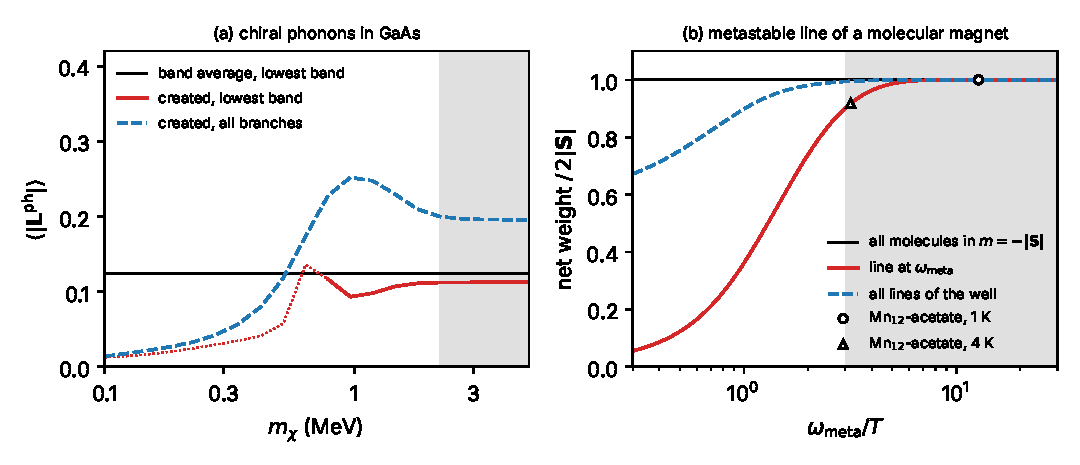
\includegraphics[width=0.98\linewidth]{figures/ch14/limit14_5a.pdf}
\captionof{figure}{(a) GaAs, from the PBE force constants of \cref{sec:5.5}. Black: the average of $|\vect{L}^{\mathrm{ph}}|$ over the lowest band, 0.124. Red: the same average weighted with the one-phonon rate of a heavy mediator coupled to nucleon number (\cref{eq:11.1-S1}, orientation-averaged halo kernel, $T = 0$), for the lowest-band phonons that the dark matter creates directly, against $\mchi$; dotted where the lowest band takes less than \SI{1}{\percent} of the rate. Blue dashed: the same for all created phonons. Gray: red within \SI{10}{\percent} of black, $\mchi \ge \SI{2.2}{MeV}$. (b) Mn$_{12}$-acetate ($|\mathbf{S}| = 10$, $D = \SI{0.454}{cm^{-1}}$, $B_4^0 = \SI{-2.0e-5}{cm^{-1}}$, \SI{1}{T}, $g_{\mathrm{ion}} = 2$, $\omega_{\mathrm{meta}} = \SI{1.098}{meV}$): net absorptive weight over $2|\mathbf{S}|$ against $\omega_{\mathrm{meta}}/T$, for thermal populations inside the upper well. Red: the line at $\omega_{\mathrm{meta}}$; blue dashed: all lines of the well, $2|\langle S_z\rangle|/2|\mathbf{S}|$. Gray: the line within \SI{10}{\percent} of $2|\mathbf{S}|$, $\omega_{\mathrm{meta}}/T \ge 3.0$. Markers: \SI{1}{K} and \SI{4}{K}.}\label{fig:14-limit-chiral}
\par}
\smallskip
Outside the gray regions the band average misstates the chirality of the phonons that a light particle creates, and a warm molecular crystal spreads the metastable weight over the lines of its well.
\end{limitbox}

\subsection{Magnetoelectric response of multiferroics}\label{sec:14.5-mf}

Hexagonal Lu$_{1-x}$Sc$_x$FeO$_3$ with $x \approx 0.4$ becomes ferroelectric at about \SI{1200}{K}. Below its magnetic ordering temperature $T_{\mathrm{CM}} \approx \SI{160}{K}$ the canted spins of its iron ions add a net magnetization parallel to the polarization. For hexagonal LuFeO$_3$ ($x = 0$), density-functional calculations give a polarization of \SI{10.5}{\micro C.cm^{-2}} along the $c$ axis and a net moment of $0.02\,\mu_B$ per iron~\cite[Sect.~IV\,A]{roising2021axion}. A crystal with both orders breaks inversion and time reversal and keeps their product. R{\o}ising and collaborators propose that an axion field shifts the magnetization of a multiferroic with both orders through the coupling of the axion to the electron, $\delta E = -\ii g_{aee}(\partial_t\phi/2m_e^2)\langle\boldsymbol{\sigma}\cdot\nabla\rangle$~\cite[Eq.~(5)]{roising2021axion}. With $\vect{p} = -\ii\nabla$ and $\boldsymbol{\sigma} = 2\vect{S}$, the spin current of \cref{eq:8.1-rows} at $\vect{q} = 0$ is $\mathcal{J}^{\alpha\alpha}_e(0) = \sum_j\vect{p}_j\cdot\vect{S}_j/m_e = -\ii\sum_j\boldsymbol{\sigma}_j\cdot\nabla_j/2m_e$, so the coupling is $(g_{aee}/m_e)(\partial_t\phi)\,\mathcal{J}^{\alpha\alpha}_e(0)$, the second term of \cref{eq:8.1-alp} at $\vect{p}_\phi \to 0$. By the Kubo formula of \cref{sec:4.2}, the spin density then responds as
\begin{equation}
  \frac{\delta\langle s^z_e(0)\rangle(\omega)}{\Vol} = \frac{g_{aee}}{m_e}\,R_{s^z\mathcal{J}}(0,\omega)\,(\partial_t\phi)(\omega) = -\ii\,\frac{g_{aee}m_\phi}{m_e}\,R_{s^z\mathcal{J}}(0,m_\phi)\,\phi(\omega) ,
  \label{eq:14.5-cross}
\end{equation}
with $R_{s^z\mathcal{J}}$ the retarded response of $s^z_e$ to $\mathcal{J}^{\alpha\alpha}_e$ and the magnetization $-2\mu_B$ times the left-hand side. The spin-density and spin-current rows have opposite signs under both time reversal and inversion, $\sigma^{\mathsf{T}}_s\sigma^{\mathsf{T}}_{\mathcal{J}} = \sigma^{\mathsf{P}}_s\sigma^{\mathsf{P}}_{\mathcal{J}} = -1$, so by \cref{eq:14.5-recip} inversion removes the block at $\vect{q} = 0$ and time reversal removes its symmetric part, the part that survives as $\omega \to 0$. The adiabatic response thus needs both symmetries broken, as in Lu$_{1-x}$Sc$_x$FeO$_3$ below $T_{\mathrm{CM}}$.

The Lehmann form of \cref{sec:4.2}, $R_{ab} = \Vol^{-1}\sum_{i,n}(p_i - p_n)\langle i|O_a^\dagger|n\rangle\langle n|O_b|i\rangle/(\omega - \omega_{ni} + \ii0^+)$, shows which states contribute. Far below $T_{\mathrm{CM}}$ the states $n$ reached at $\vect{q} = 0$ from the ordered state are its uniform magnon modes, in linear spin-wave theory as in \cref{sec:14.3}. Each mode $\nu$ with both matrix elements nonzero contributes a pair of poles at $\pm\omega_\nu$, which combine for real matrix elements into a term proportional to $2\omega_\nu/(\omega^2 - \omega_\nu^2)$. Two conditions restrict the modes. If the Hamiltonian conserves the total spin component $S^z_{\mathrm{tot}}$ and $s^z_e(0) = \lambda_SS^z_{\mathrm{tot}}$, then $s^z_e(0)$ has no time dependence and $R_{s^z\mathcal{J}}(0,\omega)$ vanishes at every $\omega \ne 0$. The response needs a spin--orbit coupling, a Dzyaloshinskii--Moriya interaction or a single-ion anisotropy that does not commute with $S^z_{\mathrm{tot}}$, such as the one that cants the spins of hexagonal Lu$_{1-x}$Sc$_x$FeO$_3$. And $\mathcal{J}^{\alpha\alpha}_e$ is odd under inversion, and it has matrix elements within the ground configuration of an ion only through a crystal field without inversion together with spin--orbit coupling (\cref{sec:14.3}). The response is thus at least of second order in spin--orbit coupling: one order for the vertex, and one or two for the breaking of $S^z_{\mathrm{tot}}$, by a Dzyaloshinskii--Moriya term or a single-ion term.

Far below $T_{\mathrm{CM}}$, where thermal magnons reduce the moment by less than \SI{10}{\percent} ($T \le 0.37\,T_{\mathrm{CM}}$ for spin $\frac52$ with nearest-neighbor exchange on a simple-cubic lattice), the Lehmann sum over the uniform magnons and their thermal population is the controlled result. Near $T_{\mathrm{CM}}$, dynamic scaling predicts the structure $R_{s^z\mathcal{J}}(0,\omega;T) = \chi_\times(T)\,\Phi(\omega\tau(T))$, with a relaxation time $\tau \propto |T - T_{\mathrm{CM}}|^{-\nu z}$, $\nu$ the correlation-length exponent and $z$ the dynamic exponent~\cite[Sect.~III\,D]{roising2021axion}; the amplitude $\chi_\times$ and the scaling function $\Phi$ of a real material are not known. The exchange, Dzyaloshinskii--Moriya and anisotropy constants of the spin model for $T \ll T_{\mathrm{CM}}$ come from DFT~$+\,U$ energy mappings, with spin--orbit coupling included for the vertex of $\mathcal{J}^{\alpha\alpha}_e$.

\subsection{Uncertainty budget of the magnetic rates}\label{sec:14.5-budget}

\Cref{tab:14-nuisances} collects the truncations and inputs of the chapter with their sizes. Near the lightest masses the anisotropy row dominates every other row by more than an order of magnitude, and it is a model, not a calculation. For absorption into the uniform mode, the shape of the sample and the width of the line set the rate, and neither depends on the spin-wave expansion. In the coherent regime the largest effects are statistical: the length of the record against $t_{\mathrm{coh}}$ and $T_2$, and whether the likelihood contains the random amplitude.
\begin{table}[tbp]
  \caption{Uncertainty budget of the magnetic rates and of the coherent regime. Classes as in \cref{tab:10-nuisances}; ``unsized'' marks an item with no size known. Sizes are for NiO, YIG, MnF$_2$, GaAs, Mn$_{12}$-acetate and $^{207}$Pb in PMN-PT as named.}
  \label{tab:14-nuisances}
  \centering\scriptsize\setlength{\tabcolsep}{3pt}
  \begin{tabular}{@{}>{\raggedright\arraybackslash}p{0.27\linewidth}>{\raggedright\arraybackslash}p{0.13\linewidth}>{\raggedright\arraybackslash}p{0.48\linewidth}>{\raggedright\arraybackslash}p{0.08\linewidth}@{}}
    \toprule
    Truncation or input & Type & Size & Section \\
    \midrule
    One-magnon weight of linear spin-wave theory & normali\-zation & high by about $\Delta S/|\vect{S}|$: \SI{7.8}{\percent} (NiO), \SI{3.1}{\percent} for $|\vect{S}| = \frac52$, \SI{16}{\percent} for $|\vect{S}| = \frac12$ & \cref{sec:14.1} \\
    Two-magnon continuum & new support & 0.073 of the one-magnon weight over the zone (NiO); $w_\parallel/w_\perp < 0.05$ below \SI{0.5}{keV} & \cref{sec:14.2} \\
    Final-state interaction of the pair & tilt; new support & about 0.04 of the spin response, moved in energy (NiO); bound pair unsized & \cref{sec:14.2} \\
    Magnetic anisotropy near the gap & threshold; tilt in $\mchi$ & NiO, \SI{5}{meV} threshold, one-constant gap \SI{4.54}{meV}: rate $\times29$ at \SI{10}{keV} (upper value), $\times1.35$ at \SI{30}{keV}, $< \SI{3}{\percent}$ above \SI{100}{keV} & \cref{sec:14.1} \\
    Exchange constants from DFT~$+\,U$ & threshold & $J_2$ of NiO 11 to \SI{27}{meV} against 19.01: magnon energies $\times0.58$ to 1.42 & \cref{sec:14.1} \\
    Magnon--phonon mixing & tilt & gap \SI{3.0}{\percent} of the crossing energy at \SI{2.83}{GHz} (YIG model); NiO unsized & \cref{sec:14.2} \\
    Thermal magnons & new support & $\ee^{-\omega_{\mathrm{gap}}/T}$, exponent $-5\times10^3$ at \SI{10}{mK} (NiO) & \cref{sec:14.1} \\
    Sample shape & threshold; normali\-zation & YIG film within \SI{10}{\percent} of the Larmor line for $B_0 \ge 4.8\,\mu_0M_{\mathrm{s}}$; weight $\times1.74$ at \SI{10}{\micro eV}; saturated sphere exact & \cref{sec:14.3} \\
    Zero-point correction to the resonance weight & normali\-zation & 5 to \SI{23}{\percent} for $|\vect{S}| = \frac32$, $\omega_A/\omega_E = 2$ to 0.3; MnF$_2$ unsized & \cref{sec:14.3} \\
    Resonance of MnF$_2$ & threshold & fitted fields \SI{7}{\percent} below the measured \SI{1.1}{meV} and \SI{9.4}{T}; peak rate unchanged & \cref{sec:14.3} \\
    Width $\varGamma_{\mathrm{M}}$ of the uniform line & normali\-zation & peak rate $\propto 1/\varGamma_{\mathrm{M}}$; $10^{-5}\omega$ for YIG assumed & \cref{sec:14.3} \\
    Spin fraction $\lambda_S$ of quenched $3d$ ions & normali\-zation & $1 - O(\xi_{\mathrm{ion}}^2/\Delta_{\mathrm{CF}}^2)$ & \cref{sec:14.3} \\
    In-medium mixing of a dark photon & normali\-zation & set by the dielectric constant and the enclosure; unsized & \cref{sec:14.3} \\
    Neutron data for quenched ions & normali\-zation & $[\lambda_S/(g_{\mathrm{ion}}/2)]^2 = 0.83$ (Ni$^{2+}$, $g_{\mathrm{ion}} = 2.2$) or 0.73 (2.34); 0.973 at \SI{5.3}{keV} & \cref{sec:14.4} \\
    Longitudinal response from neutron data & new support & needs the localized-moment form or the isotropy hypothesis & \cref{sec:14.4} \\
    Record length against $t_{\mathrm{coh}}$ and $1/\varGamma_{\mathrm{tg}}$ & normali\-zation & mean within \SI{10}{\percent} of the golden rule for $t_{\mathrm{int}} \ge 13\,t_{\mathrm{coh}}$ ($T_2 \to \infty$) to $t_{\mathrm{coh}}$ ($T_2 = 0.1\,t_{\mathrm{coh}}$) & \cref{sec:14.6} \\
    Field amplitude fixed instead of Rayleigh & normali\-zation & limit too strong by 1.99 below $t_{\mathrm{coh}}$, 1.015 at $100\,t_{\mathrm{coh}}$; 2.73 at the detection threshold & \cref{sec:14.6} \\
    Linearized Bloch equation & normali\-zation & $(\Omega_{\mathrm{Rabi}}t)^2/6$ in the transient; \SI{30}{\percent} saturation at the PMN-PT threshold & \cref{sec:14.6} \\
    Inhomogeneous broadening; effective field $E^*$ & normali\-zation & $u_{\mathrm{sp}} = 3.8\times10^{-4}$; $E^*$ about \SI{50}{\percent} ($^{207}$Pb in PMN-PT) & \cref{sec:14.6} \\
    Line shape of the halo & tilt & standard halo only; unsized & \cref{sec:14.6} \\
    Chiral phonons as a band average & normali\-zation & GaAs 0.124, $\pm\SI{40}{\percent}$ with the dipole part of the force constants; rate-weighted within \SI{10}{\percent} only for $\mchi \ge \SI{2.2}{MeV}$; decay branching unsized & \cref{sec:14.5} \\
    Upper-well population of a molecular magnet & normali\-zation & Mn$_{12}$-acetate at \SI{1}{T}: line keeps \SI{90}{\percent} of $2|\vect{S}|$ below \SI{4.2}{K} & \cref{sec:14.5} \\
    Multiferroic response near $T_{\mathrm{CM}}$ & normali\-zation; tilt & unsized & \cref{sec:14.5} \\
    \bottomrule
  \end{tabular}
\end{table}

\section*{Summary}

A dark-matter particle that couples to the electron spin creates one magnon through the transverse spin, at leading order in $1/|\vect{S}|$ (\cref{sec:14.1}). In a two-sublattice antiferromagnet the one-magnon response carries the weight $w^{\mathrm{M}}_{\vect{q}} = |\vect{S}|(A_{\vect{q}} - B_{\vect{q}})/\omega^{\mathrm{M}}_{\vect{q}}$, which suppresses magnons near the zone center and enhances them near the ordering wavevector: 0.024 against 42 for magnons of \SI{5}{meV} in NiO. For NiO at $\sigmae = \SI{e-40}{cm^2}$ it opens near \SI{7.3}{keV} for a \SI{5}{meV} threshold and peaks at $3.2\times10^3$ events per kilogram-year near \SI{3}{MeV}. Near its edge the rate depends on the magnetic anisotropy, which the Heisenberg model leaves out. The spin-length sum rule estimates that linear spin-wave theory overstates the one-magnon weight by $\Delta S/|\vect{S}|$ at the next order, \SI{7.8}{\percent} for NiO, where the zero-point reduction $\Delta S = 0.078$ is that of four interleaved simple-cubic antiferromagnets.

The longitudinal spin creates magnon pairs (\cref{sec:14.2}). Their weight vanishes in a ferromagnet and at $\vect{q} = 0$, grows as $q^2$, and averages to 0.073 of the one-magnon weight in NiO, the part of the $\Delta S/|\vect{S}| = 0.078$ moved out of the one-magnon line that arrives in the continuum (the two differ by $\Delta S^2$). Because a pair shares its momentum, it reaches the energy $\frac12\mchi v^2$ at any mass, and the two-magnon channel opens at masses lower by $v_{\mathrm{max}}^2/4c_{\mathrm{M}}(v_{\mathrm{max}} - c_{\mathrm{M}})$, a factor 5.1 for NiO. Final-state interactions move the pair weight within the continuum without changing its integral; whether NiO has a bound pair is open. A magnon mixes with a phonon at linear order only through the dependence of the anisotropy energy on strain, which spin--orbit coupling and the dipolar interaction provide; the strain dependence of the exchange couples a phonon only to magnon pairs. The hybrids carry an off-diagonal spin--nuclear response that saturates the interference bound of \cref{sec:8.3}.

A boson absorbed at $\vect{k} \to 0$ drives the uniform precession (\cref{sec:14.3}). When the exchange is invariant under spin rotations, the uniform transverse spin response is one line at the Larmor frequency, with weight $2\langle S^z_{\mathrm{tot}}\rangle$, at any spin and temperature. The spin couples through $\lambda_S$, the fraction of the ionic angular momentum carried by the spin, which equals $g_J - 1$ only within a $J$ multiplet and is one for quenched $3d$ ions. The shape of the sample moves the line to the Kittel frequency and reweights its polarizations. For YIG at \SI{10}{\micro eV} and $g_{aee} = 10^{-13}$, with an assumed line width of $10^{-5}$ of the frequency, the peak rate is \SI{3.6}{s^{-1}.kg^{-1}}. An antiferromagnet absorbs at its resonance with the exchange-suppressed weight $|\vect{S}|\omega_{\mathrm{AFMR}}/(2\omega_E + \omega_A)$ per pair of sublattices, about $0.1\,|\vect{S}|$ in MnF$_2$, whose resonance lies at the measured \SI{1.1}{meV}.

Measured neutron spectra can replace a computed spin response, within limits (\cref{sec:14.4}). The magnetic cross-section at a given momentum transfer contains only the part of the spin response transverse to it, so without a model of the spin density no neutron measurement, polarized or not, gives the longitudinal element $\hat{\vect{q}}\cdot S\cdot\hat{\vect{q}}$. Within the localized-moment model, transverse data at several wavevectors $\vect{q} + \vect{G}$ fix the full tensor, and an isotropy hypothesis recovers it from two scattering angles. For quenched ions the neutron sees the moment with the spectroscopic $g$, the dark matter the spin, and the factor $[\lambda_S/(g_{\mathrm{ion}}/2)]^2$ converts one into the other, 0.83 for Ni$^{2+}$ at $g_{\mathrm{ion}} = 2.2$ and 0.73 at 2.34.

Targets without inversion or time-reversal symmetry add responses that a collinear magnet lacks (\cref{sec:14.5}). The current response of a chiral crystal acquires a part odd in $\vect{q}$, the finite-momentum optical activity, and the point group decides whether it exists; in $\alpha$-quartz the orientation-averaged gyration is only $-0.045$ of its value along the optic axis. Phonons of the lowest band of GaAs carry on average 0.12 units of angular momentum. Single-molecule magnets offer metastable lines, such as the line of Mn$_{12}$-acetate at \SI{1.098}{meV} in \SI{1}{T}, which keeps \SI{90}{\percent} of its weight below \SI{4.2}{K}. A multiferroic below its ordering temperature has a magnetoelectric cross response; near that temperature the response is open.

An ultralight field is a classical Gaussian wave, coherent for $t_{\mathrm{coh}} = 1/m_\phi v_0^2$, \SI{1.04}{s} at \SI{1}{neV} (\cref{sec:14.6}). Its average reproduces the golden-rule rate for records longer than the shorter of $t_{\mathrm{coh}}$ and the inverse width of the target's line, while a single record matches the ensemble only beyond $t_{\mathrm{coh}}$. A polarized nuclear-spin ensemble driven by the gradient or the dipole coupling of an axion-like field obeys the Bloch equations. Its transverse magnetization grows as $\Omega_{\mathrm{Rabi}}M_0t$ and saturates at $\Omega_{\mathrm{Rabi}}M_0T_2$, and a Gaussian drive turns the linear growth into a random walk once the record exceeds $t_{\mathrm{coh}}$. Each periodogram bin of signal plus noise is exponentially distributed. The resulting likelihood gives sensitivities that scale as $t_{\mathrm{int}}^{-1/2}$ below the coherence time and as $(t_{\mathrm{int}}t_{\mathrm{coh}})^{-1/4}$ above it, and it already contains the random amplitude, which a fixed-amplitude analysis misses by a factor 1.99 for the median limit and 2.73 at the detection threshold.

\Cref{tab:14-nuisances} collects the truncations and inputs of the chapter with their sizes. Near the lightest masses the anisotropy row dominates every other by more than an order of magnitude, and it is a model, not a calculation. For absorption into the uniform mode, the shape of the sample and the width of the line set the rate, and neither depends on the spin-wave expansion. In the coherent regime the largest effects are statistical: the length of the record against $t_{\mathrm{coh}}$ and $T_2$, and whether the likelihood contains the random amplitude.

\begin{table}[tbp]
  \caption{Uncertainty budget of the magnetic rates and of the coherent regime. Type in the classes of \cref{sec:8.8}: normalization, tilt (in $\omega$ or in the dark-matter mass), threshold and new support; ``unsized'' marks an item with no size known. Sizes are for NiO, YIG, MnF$_2$, GaAs, Mn$_{12}$-acetate and $^{207}$Pb in PMN-PT as named.}
  \label{tab:14-nuisances}
  \centering\scriptsize\setlength{\tabcolsep}{3pt}
  \begin{tabular}{@{}>{\raggedright\arraybackslash}p{0.27\linewidth}>{\raggedright\arraybackslash}p{0.13\linewidth}>{\raggedright\arraybackslash}p{0.48\linewidth}>{\raggedright\arraybackslash}p{0.08\linewidth}@{}}
    \toprule
    Truncation or input & Type & Size & Section \\
    \midrule
    One-magnon weight of linear spin-wave theory & normali\-zation & high by about $\Delta S/|\vect{S}|$: \SI{7.8}{\percent} (NiO), \SI{3.1}{\percent} for $|\vect{S}| = \frac52$, \SI{16}{\percent} for $|\vect{S}| = \frac12$ & \cref{sec:14.1} \\
    Two-magnon continuum & new support & 0.073 of the one-magnon weight over the zone (NiO); $w_\parallel/w_\perp < 0.05$ below \SI{0.5}{keV} & \cref{sec:14.2} \\
    Final-state interaction of the pair & tilt; new support & about 0.04 of the spin response, moved in energy (NiO); bound pair unsized & \cref{sec:14.2} \\
    Magnetic anisotropy near the gap & threshold; tilt in $\mchi$ & NiO, \SI{5}{meV} threshold, one-constant gap \SI{4.54}{meV}: rate $\times29$ at \SI{10}{keV} (upper value), $\times1.35$ at \SI{30}{keV}, $< \SI{3}{\percent}$ above \SI{100}{keV} & \cref{sec:14.1} \\
    Exchange constants from DFT~$+\,U$ & threshold & $J_2$ of NiO 11 to \SI{27}{meV} against 19.01: magnon energies $\times0.58$ to 1.42 & \cref{sec:14.1} \\
    Magnon--phonon mixing & tilt & gap \SI{3.0}{\percent} of the crossing energy at \SI{2.83}{GHz} (YIG model); NiO unsized & \cref{sec:14.2} \\
    Thermal magnons & new support & $\ee^{-\omega_{\mathrm{gap}}/T}$, exponent $-5\times10^3$ at \SI{10}{mK} (NiO) & \cref{sec:14.1} \\
    Sample shape & threshold; normali\-zation & YIG film within \SI{10}{\percent} of the Larmor line for $B_0 \ge 4.8\,\mu_0M_{\mathrm{s}}$; weight $\times1.74$ at \SI{10}{\micro eV}; saturated sphere exact & \cref{sec:14.3} \\
    Zero-point correction to the resonance weight & normali\-zation & 5 to \SI{23}{\percent} for $|\vect{S}| = \frac32$, $\omega_A/\omega_E = 2$ to 0.3; MnF$_2$ unsized & \cref{sec:14.3} \\
    Resonance of MnF$_2$ & threshold & fitted fields \SI{7}{\percent} below the measured \SI{1.1}{meV} and \SI{9.4}{T}; peak rate unchanged & \cref{sec:14.3} \\
    Width $\varGamma_{\mathrm{M}}$ of the uniform line & normali\-zation & peak rate $\propto 1/\varGamma_{\mathrm{M}}$; $10^{-5}\omega$ for YIG assumed & \cref{sec:14.3} \\
    Spin fraction $\lambda_S$ of quenched $3d$ ions & normali\-zation & $1 - O(\xi_{\mathrm{ion}}^2/\Delta_{\mathrm{CF}}^2)$ & \cref{sec:14.3} \\
    In-medium mixing of a dark photon & normali\-zation & set by the dielectric constant and the enclosure; unsized & \cref{sec:14.3} \\
    Neutron data for quenched ions & normali\-zation & $[\lambda_S/(g_{\mathrm{ion}}/2)]^2 = 0.83$ (Ni$^{2+}$, $g_{\mathrm{ion}} = 2.2$) or 0.73 (2.34); 0.973 at \SI{5.3}{keV} & \cref{sec:14.4} \\
    Longitudinal response from neutron data & new support & needs the localized-moment form or the isotropy hypothesis & \cref{sec:14.4} \\
    Chiral phonons as a band average & normali\-zation & GaAs 0.124, $\pm\SI{40}{\percent}$ with the dipole part of the force constants; rate-weighted within \SI{10}{\percent} only for $\mchi \ge \SI{2.2}{MeV}$; decay branching unsized & \cref{sec:14.5} \\
    Upper-well population of a molecular magnet & normali\-zation & Mn$_{12}$-acetate at \SI{1}{T}: line keeps \SI{90}{\percent} of $2|\vect{S}|$ below \SI{4.2}{K} & \cref{sec:14.5} \\
    Multiferroic response near $T_{\mathrm{CM}}$ & normali\-zation; tilt & unsized & \cref{sec:14.5} \\
    Record length against $t_{\mathrm{coh}}$ and $1/\varGamma_{\mathrm{tg}}$ & normali\-zation & mean within \SI{10}{\percent} of the golden rule for $t_{\mathrm{int}} \ge 13\,t_{\mathrm{coh}}$ ($T_2 \to \infty$) to $t_{\mathrm{coh}}$ ($T_2 = 0.1\,t_{\mathrm{coh}}$) & \cref{sec:14.6} \\
    Field amplitude fixed instead of Rayleigh & normali\-zation & limit too strong by 1.99 below $t_{\mathrm{coh}}$, 1.015 at $100\,t_{\mathrm{coh}}$; 2.73 at the detection threshold & \cref{sec:14.6} \\
    Linearized Bloch equation & normali\-zation & $(\Omega_{\mathrm{Rabi}}t)^2/6$ in the transient; \SI{30}{\percent} saturation at the PMN-PT threshold & \cref{sec:14.6} \\
    Inhomogeneous broadening; effective field $E^*$ & normali\-zation & $u_{\mathrm{sp}} = 3.8\times10^{-4}$; $E^*$ about \SI{50}{\percent} ($^{207}$Pb in PMN-PT) & \cref{sec:14.6} \\
    Line shape of the halo & tilt & standard halo only; unsized & \cref{sec:14.6} \\
    \bottomrule
  \end{tabular}
\end{table}

\printbibliography[heading=subbibliography]
